% Options for packages loaded elsewhere
\PassOptionsToPackage{unicode}{hyperref}
\PassOptionsToPackage{hyphens}{url}
%
\documentclass[
]{article}
\usepackage{amsmath,amssymb}
\usepackage{iftex}
\ifPDFTeX
  \usepackage[T1]{fontenc}
  \usepackage[utf8]{inputenc}
  \usepackage{textcomp} % provide euro and other symbols
\else % if luatex or xetex
  \usepackage{unicode-math} % this also loads fontspec
  \defaultfontfeatures{Scale=MatchLowercase}
  \defaultfontfeatures[\rmfamily]{Ligatures=TeX,Scale=1}
\fi
\usepackage{lmodern}
\ifPDFTeX\else
  % xetex/luatex font selection
\fi
% Use upquote if available, for straight quotes in verbatim environments
\IfFileExists{upquote.sty}{\usepackage{upquote}}{}
\IfFileExists{microtype.sty}{% use microtype if available
  \usepackage[]{microtype}
  \UseMicrotypeSet[protrusion]{basicmath} % disable protrusion for tt fonts
}{}
\makeatletter
\@ifundefined{KOMAClassName}{% if non-KOMA class
  \IfFileExists{parskip.sty}{%
    \usepackage{parskip}
  }{% else
    \setlength{\parindent}{0pt}
    \setlength{\parskip}{6pt plus 2pt minus 1pt}}
}{% if KOMA class
  \KOMAoptions{parskip=half}}
\makeatother
\usepackage{xcolor}
\usepackage[margin=1in]{geometry}
\usepackage{color}
\usepackage{fancyvrb}
\newcommand{\VerbBar}{|}
\newcommand{\VERB}{\Verb[commandchars=\\\{\}]}
\DefineVerbatimEnvironment{Highlighting}{Verbatim}{commandchars=\\\{\}}
% Add ',fontsize=\small' for more characters per line
\usepackage{framed}
\definecolor{shadecolor}{RGB}{248,248,248}
\newenvironment{Shaded}{\begin{snugshade}}{\end{snugshade}}
\newcommand{\AlertTok}[1]{\textcolor[rgb]{0.94,0.16,0.16}{#1}}
\newcommand{\AnnotationTok}[1]{\textcolor[rgb]{0.56,0.35,0.01}{\textbf{\textit{#1}}}}
\newcommand{\AttributeTok}[1]{\textcolor[rgb]{0.13,0.29,0.53}{#1}}
\newcommand{\BaseNTok}[1]{\textcolor[rgb]{0.00,0.00,0.81}{#1}}
\newcommand{\BuiltInTok}[1]{#1}
\newcommand{\CharTok}[1]{\textcolor[rgb]{0.31,0.60,0.02}{#1}}
\newcommand{\CommentTok}[1]{\textcolor[rgb]{0.56,0.35,0.01}{\textit{#1}}}
\newcommand{\CommentVarTok}[1]{\textcolor[rgb]{0.56,0.35,0.01}{\textbf{\textit{#1}}}}
\newcommand{\ConstantTok}[1]{\textcolor[rgb]{0.56,0.35,0.01}{#1}}
\newcommand{\ControlFlowTok}[1]{\textcolor[rgb]{0.13,0.29,0.53}{\textbf{#1}}}
\newcommand{\DataTypeTok}[1]{\textcolor[rgb]{0.13,0.29,0.53}{#1}}
\newcommand{\DecValTok}[1]{\textcolor[rgb]{0.00,0.00,0.81}{#1}}
\newcommand{\DocumentationTok}[1]{\textcolor[rgb]{0.56,0.35,0.01}{\textbf{\textit{#1}}}}
\newcommand{\ErrorTok}[1]{\textcolor[rgb]{0.64,0.00,0.00}{\textbf{#1}}}
\newcommand{\ExtensionTok}[1]{#1}
\newcommand{\FloatTok}[1]{\textcolor[rgb]{0.00,0.00,0.81}{#1}}
\newcommand{\FunctionTok}[1]{\textcolor[rgb]{0.13,0.29,0.53}{\textbf{#1}}}
\newcommand{\ImportTok}[1]{#1}
\newcommand{\InformationTok}[1]{\textcolor[rgb]{0.56,0.35,0.01}{\textbf{\textit{#1}}}}
\newcommand{\KeywordTok}[1]{\textcolor[rgb]{0.13,0.29,0.53}{\textbf{#1}}}
\newcommand{\NormalTok}[1]{#1}
\newcommand{\OperatorTok}[1]{\textcolor[rgb]{0.81,0.36,0.00}{\textbf{#1}}}
\newcommand{\OtherTok}[1]{\textcolor[rgb]{0.56,0.35,0.01}{#1}}
\newcommand{\PreprocessorTok}[1]{\textcolor[rgb]{0.56,0.35,0.01}{\textit{#1}}}
\newcommand{\RegionMarkerTok}[1]{#1}
\newcommand{\SpecialCharTok}[1]{\textcolor[rgb]{0.81,0.36,0.00}{\textbf{#1}}}
\newcommand{\SpecialStringTok}[1]{\textcolor[rgb]{0.31,0.60,0.02}{#1}}
\newcommand{\StringTok}[1]{\textcolor[rgb]{0.31,0.60,0.02}{#1}}
\newcommand{\VariableTok}[1]{\textcolor[rgb]{0.00,0.00,0.00}{#1}}
\newcommand{\VerbatimStringTok}[1]{\textcolor[rgb]{0.31,0.60,0.02}{#1}}
\newcommand{\WarningTok}[1]{\textcolor[rgb]{0.56,0.35,0.01}{\textbf{\textit{#1}}}}
\usepackage{graphicx}
\makeatletter
\def\maxwidth{\ifdim\Gin@nat@width>\linewidth\linewidth\else\Gin@nat@width\fi}
\def\maxheight{\ifdim\Gin@nat@height>\textheight\textheight\else\Gin@nat@height\fi}
\makeatother
% Scale images if necessary, so that they will not overflow the page
% margins by default, and it is still possible to overwrite the defaults
% using explicit options in \includegraphics[width, height, ...]{}
\setkeys{Gin}{width=\maxwidth,height=\maxheight,keepaspectratio}
% Set default figure placement to htbp
\makeatletter
\def\fps@figure{htbp}
\makeatother
\setlength{\emergencystretch}{3em} % prevent overfull lines
\providecommand{\tightlist}{%
  \setlength{\itemsep}{0pt}\setlength{\parskip}{0pt}}
\setcounter{secnumdepth}{5}
\usepackage{pdfpages}
\usepackage{tcolorbox}
\usepackage{graphicx}
\usepackage{setspace}
\usepackage{booktabs}
\usepackage{caption}
\usepackage{longtable}
\usepackage{multirow}
\usepackage{multicol}
\usepackage{colortbl}
\usepackage{hhline}
\newlength\Oldarrayrulewidth
\newlength\Oldtabcolsep
\usepackage{array}
\usepackage{hyperref}
\usepackage{float}
\usepackage{wrapfig}
\ifLuaTeX
  \usepackage{selnolig}  % disable illegal ligatures
\fi
\IfFileExists{bookmark.sty}{\usepackage{bookmark}}{\usepackage{hyperref}}
\IfFileExists{xurl.sty}{\usepackage{xurl}}{} % add URL line breaks if available
\urlstyle{same}
\hypersetup{
  hidelinks,
  pdfcreator={LaTeX via pandoc}}

\author{}
\date{\vspace{-2.5em}}

\begin{document}


\includepdf{pagedegarde}

\setstretch{1.5}

\renewcommand{\contentsname}{\textcolor{blue}{Table des matières}}

\textcolor{blue}{\tableofcontents}

\newpage

\textcolor{blue}{\section*{RESUME}\addcontentsline{toc}{section}{RESUME}}

Ce projet vise à étudier les bioénergies durables pour les PME
agroalimentaires en Afrique de l'Ouest en trois parties distinctes.

Dans la première partie, nous analyserons les bioénergies durables en
utilisant un jeu de données de 250 observations et 33 variables du
fichier ``Base\_Partie1.xlsx''. L'objectif est d'obtenir des
statistiques descriptives et de cartographier leur répartition
géographique.

La deuxième partie traitera du nettoyage et de l'analyse des données
avec un ensemble de données artificielles du fichier
``Base\_Partie2.xlsx''. Nous préparerons les données et créerons des
visualisations pour mieux comprendre les relations entre les variables.

Enfin, dans la troisième partie, nous développerons une application R
Shiny interactive pour visualiser les événements politiques et les
violences en Afrique de l'Ouest en utilisant la base de données
``ACLED-Western\_Africa.csv''. L'application permettra aux utilisateurs
de filtrer et de localiser ces événements sur une carte interactive.

En résumé, ce projet explore les opportunités de bioénergies durables
pour les PME agroalimentaires en Afrique de l'Ouest grâce à des analyses
statistiques, des visualisations et une application interactive.

\newpage

\begin{Shaded}
\begin{Highlighting}[]
\DocumentationTok{\#\#\#\#\#\#\#\#\#\#\#\#\#\#\#\#\#\#\#\#\#\#\#\#\#\#\#\#\#\#\#\#\#\#\#\#\#\#\#\#\#\#\#\#\#\#\#\#\#\#\#\#\#\#\#\#\#\#\#\#\#\#\#\#\#\#\#\#\#\#\#\#\#\#\#\#\#\#\#\#\#\#\#\#\#\#\#\#}
\CommentTok{\#                                                             }
\CommentTok{\# {-}{-}{-}{-}{-}{-}{-}{-}{-}{-}{-}{-}{-}{-}{-}{-}{-}{-}{-}{-}{-}{-}{-}{-}{-} CHARGEMENT DES PACKAGES UTILISES{-}{-}{-}{-}{-}{-}{-}{-}{-}{-}{-}{-}{-}{-}{-}{-}}
\CommentTok{\#                                                             }
\DocumentationTok{\#\#\#\#\#\#\#\#\#\#\#\#\#\#\#\#\#\#\#\#\#\#\#\#\#\#\#\#\#\#\#\#\#\#\#\#\#\#\#\#\#\#\#\#\#\#\#\#\#\#\#\#\#\#\#\#\#\#\#\#\#\#\#\#\#\#\#\#\#\#\#\#\#\#\#\#\#\#\#\#\#\#\#\#\#\#\#\#}

\CommentTok{\# {-}{-}{-}{-}{-}{-}{-}{-}{-}{-}{-}{-}{-}{-}{-}{-}{-}{-}{-}{-}{-}{-}{-}{-}{-}{-}MANIPULATION DE DONNEES :{-}{-}{-}{-}{-}{-}{-}{-}{-}{-}{-}{-}{-}{-}{-}{-}{-}{-}{-}{-}{-}{-}{-}{-}{-}{-}{-}{-}{-}}
\FunctionTok{library}\NormalTok{(dplyr)}
\FunctionTok{library}\NormalTok{(tidyverse)}
\FunctionTok{library}\NormalTok{(janitor)}

\CommentTok{\# {-}{-}{-}{-}{-}{-}{-}{-}{-}{-}{-}{-}{-}{-}{-}{-}{-}{-}{-}{-}{-}{-}{-}{-}VISUILISATION DE DONNEES :{-}{-}{-}{-}{-}{-}{-}{-}{-}{-}{-}{-}{-}{-}{-}{-}{-}{-}{-}{-}{-}{-}{-}{-}{-}{-}{-}{-}{-}{-}{-}{-}}
\FunctionTok{library}\NormalTok{(ggplot2)}
\FunctionTok{library}\NormalTok{(viridis)}
\FunctionTok{library}\NormalTok{(ggnewscale)}
\FunctionTok{library}\NormalTok{(ggspatial)}
\FunctionTok{library}\NormalTok{(scales)}
\FunctionTok{library}\NormalTok{(visdat)}
\FunctionTok{library}\NormalTok{(ggpirate)}\CommentTok{\#devtools::install\_github("mikabr/ggpirate")}


\CommentTok{\#{-}{-}{-}{-}{-}{-}{-}{-}{-}{-}{-}{-}{-}{-}{-}{-}{-}{-}{-}{-}{-}{-}{-}{-}{-}{-}TABLEAU ET RESUMES DE DONNEES :{-}{-}{-}{-}{-}{-}{-}{-}{-}{-}{-}{-}{-}{-}{-}{-}{-}{-}{-}{-}{-}{-}{-}{-}{-}{-}{-}{-}}
\FunctionTok{library}\NormalTok{(gt)}
\FunctionTok{library}\NormalTok{(flextable)}
\FunctionTok{library}\NormalTok{(gtsummary)}


\CommentTok{\# {-}{-}{-}{-}{-}{-}{-}{-}{-}{-}{-}{-}{-}{-}{-}{-}{-}{-}{-}{-}{-}{-}{-}{-}{-}{-}LECTURE DE DONNEES :{-}{-}{-}{-}{-}{-}{-}{-}{-}{-}{-}{-}{-}{-}{-}{-}{-}{-}{-}{-}{-}{-}{-}{-}{-}{-}{-}{-}{-}{-}{-}{-}}
\FunctionTok{library}\NormalTok{(readxl)}


\CommentTok{\# {-}{-}{-}{-}{-}{-}{-}{-}{-}{-}{-}{-}{-}{-}{-}{-}{-}{-}{-}{-}{-}{-}{-}{-}GESTION DE DONNEES SPATIALES :{-}{-}{-}{-}{-}{-}{-}{-}{-}{-}{-}{-}{-}{-}{-}{-}{-}{-}{-}{-}{-}{-}{-}{-}{-}{-}}
\FunctionTok{library}\NormalTok{(tmap)}
\FunctionTok{library}\NormalTok{(raster)}
\FunctionTok{library}\NormalTok{(leaflet)}
\FunctionTok{library}\NormalTok{(sf)}


\CommentTok{\# {-}{-}{-}{-}{-}{-}{-}{-}{-}{-}{-}{-}{-}{-}{-}{-}{-}{-}{-}{-}{-}{-}GESTION DE DISPOSITION DES GRAPHIQUES :{-}{-}{-}{-}{-}{-}{-}{-}{-}{-}{-}{-}{-}{-}{-}{-}{-}{-}{-}{-}{-}{-}{-}{-}{-}{-}}
\FunctionTok{library}\NormalTok{(gridExtra)}


\CommentTok{\#}
\end{Highlighting}
\end{Shaded}

\newpage

\textcolor{blue}{\section*{PARTIE I}\addcontentsline{toc}{section}{PARTIE I}}

\textcolor{blue}{\section*{PREPARATION DES DONNEES}\addcontentsline{toc}{section}{PREPARATION DES DONNEES}}

\textcolor{blue}{\section{DESCRIPTION}}

\textcolor{blue}{\subsection{Importation et mise en forme}}

\textcolor{blue}{\subsection{Importation de la base de donnée sous le nom “projet” et stockée dans un objet de type data.frame}}

\begin{Shaded}
\begin{Highlighting}[]
\CommentTok{\#{-}{-}{-}{-}{-}{-}{-}{-}{-}{-}{-}{-}{-}{-}{-}{-}{-}{-}{-}{-}{-}{-}{-}{-}{-}{-}{-}{-}{-}{-}{-}{-}{-}{-}{-}{-}{-}{-}{-}{-}{-}{-}{-}{-}{-}{-}{-}{-}{-}{-}{-}{-}{-}{-}{-}{-}{-}{-}{-}{-}{-}{-}{-}{-}{-}{-}{-}{-}{-}{-}{-}{-}{-}{-}{-}{-}{-}{-}{-}{-}{-}{-}{-}{-}{-}{-}{-}}
\CommentTok{\# lecture du fichier Excel "Base\_Partie 1.xlsx" :IMPORTATION  }
\CommentTok{\#{-}{-}{-}{-}{-}{-}{-}{-}{-}{-}{-}{-}{-}{-}{-}{-}{-}{-}{-}{-}{-}{-}{-}{-}{-}{-}{-}{-}{-}{-}{-}{-}{-}{-}{-}{-}{-}{-}{-}{-}{-}{-}{-}{-}{-}{-}{-}{-}{-}{-}{-}{-}{-}{-}{-}{-}{-}{-}{-}{-}{-}{-}{-}{-}{-}{-}{-}{-}{-}{-}{-}{-}{-}{-}{-}{-}{-}{-}{-}{-}{-}{-}{-}{-}{-}{-}{-}}

\NormalTok{projet }\OtherTok{\textless{}{-}} \FunctionTok{read\_excel}\NormalTok{(}\StringTok{"Base\_Partie 1.xlsx"}\NormalTok{)}

\CommentTok{\#}
\end{Highlighting}
\end{Shaded}

• Vérifiaction de l'id unique

\begin{Shaded}
\begin{Highlighting}[]
\CommentTok{\# {-}{-}{-}{-}{-}{-}{-}{-}{-}{-}{-}{-}{-}{-}{-}{-}{-}{-}{-}{-}{-}{-}{-}{-}{-}{-}{-}{-}{-}{-}{-}{-}{-}{-}{-}{-}{-}{-}{-}{-}{-}{-}{-}{-}{-}{-}{-}{-}{-}{-}{-}{-}{-}{-}{-}{-}{-}{-}{-}{-}{-}{-}{-}{-}{-}{-}{-}{-}{-}{-}{-}{-}{-}{-}{-}{-}{-}{-}{-}{-}{-}{-}{-}{-}{-}{-}{-}{-}}
\CommentTok{\#  RECHERCHE DE DOUBLONS PARMI LES IDENTIFIANT                }
\CommentTok{\#{-}{-}{-}{-}{-}{-}{-}{-}{-}{-}{-}{-}{-}{-}{-}{-}{-}{-}{-}{-}{-}{-}{-}{-}{-}{-}{-}{-}{-}{-}{-}{-}{-}{-}{-}{-}{-}{-}{-}{-}{-}{-}{-}{-}{-}{-}{-}{-}{-}{-}{-}{-}{-}{-}{-}{-}{-}{-}{-}{-}{-}{-}{-}{-}{-}{-}{-}{-}{-}{-}{-}{-}{-}{-}{-}{-}{-}{-}{-}{-}{-}{-}{-}{-}{-}{-}{-}{-}}

\NormalTok{projet }\SpecialCharTok{\%\textgreater{}\%} 
  
\NormalTok{  janitor}\SpecialCharTok{::}\FunctionTok{get\_dupes}\NormalTok{(key) }
\end{Highlighting}
\end{Shaded}

\begin{verbatim}
## # A tibble: 0 x 34
## # i 34 variables: key <chr>, dupe_count <int>, q1 <chr>, q2 <chr>, q23 <chr>,
## #   q24 <dbl>, q24a_1 <dbl>, q24a_2 <dbl>, q24a_3 <dbl>, q24a_4 <dbl>,
## #   q24a_5 <dbl>, q24a_6 <dbl>, q24a_7 <dbl>, q24a_9 <dbl>, q24a_10 <dbl>,
## #   q25 <chr>, q26 <dbl>, q12 <chr>, q14b <chr>, q16 <chr>, q17 <chr>,
## #   q19 <chr>, q20 <chr>, filiere_1 <dbl>, filiere_2 <dbl>, filiere_3 <dbl>,
## #   filiere_4 <dbl>, q8 <chr>, q81 <chr>, gps_menlatitude <dbl>,
## #   gps_menlongitude <dbl>, submissiondate <dttm>, start <dttm>, ...
\end{verbatim}

\begin{Shaded}
\begin{Highlighting}[]
\CommentTok{\#}
\end{Highlighting}
\end{Shaded}

\textcolor{blue}{\subsection{Résumer des valeurs manquantes par variable}}

\begin{Shaded}
\begin{Highlighting}[]
\CommentTok{\# {-}{-}{-}{-}{-}{-}{-}{-}{-}{-}{-}{-}{-}{-}{-}{-}{-}{-}{-}{-}{-}{-}{-}{-}{-}{-}{-}{-}Étape 1: {-}{-}{-}{-}{-}{-}{-}{-}{-}{-}{-}{-}{-}{-}{-}{-}{-}{-}{-}{-}{-}{-}{-}{-}{-}{-}{-}{-}{-}{-}{-}{-}{-}{-}{-}{-}{-}{-}{-}{-}{-}{-}{-}{-}{-}{-}{-}{-}{-}{-}}
\CommentTok{\#   Compter le nombre de valeurs manquantes dans chaque       }
\CommentTok{\#          colonne du dataframe "projet"                      }
\CommentTok{\#{-}{-}{-}{-}{-}{-}{-}{-}{-}{-}{-}{-}{-}{-}{-}{-}{-}{-}{-}{-}{-}{-}{-}{-}{-}{-}{-}{-}{-}{-}{-}{-}{-}{-}{-}{-}{-}{-}{-}{-}{-}{-}{-}{-}{-}{-}{-}{-}{-}{-}{-}{-}{-}{-}{-}{-}{-}{-}{-}{-}{-}{-}{-}{-}{-}{-}{-}{-}{-}{-}{-}{-}{-}{-}{-}{-}{-}{-}{-}{-}{-}{-}{-}}

\NormalTok{projet\_summary }\OtherTok{\textless{}{-}}\NormalTok{ projet }\SpecialCharTok{\%\textgreater{}\%}
  
  \FunctionTok{summarise}\NormalTok{(}\FunctionTok{across}\NormalTok{(}\FunctionTok{everything}\NormalTok{(), }\SpecialCharTok{\textasciitilde{}}\FunctionTok{sum}\NormalTok{(}\FunctionTok{is.na}\NormalTok{(.))))}


\CommentTok{\# {-}{-}{-}{-}{-}{-}{-}{-}{-}{-}{-}{-}{-}{-}{-}{-}{-}{-}{-}{-}{-}{-}{-}{-}{-}{-}{-}Étape 2: {-}{-}{-}{-}{-}{-}{-}{-}{-}{-}{-}{-}{-}{-}{-}{-}{-}{-}{-}{-}{-}{-}{-}{-}{-}{-}{-}{-}{-}{-}{-}{-}{-}{-}{-}{-}{-}{-}{-}{-}{-}{-}{-}{-}{-}{-}{-}{-}{-}{-}{-}}
\CommentTok{\#   Transformer le dataframe en un format "long" avec         }
\CommentTok{\#     les noms de colonnes d\textquotesingle{}origine et le nombre             }
\CommentTok{\#           de valeurs manquantes                             }
\CommentTok{\#{-}{-}{-}{-}{-}{-}{-}{-}{-}{-}{-}{-}{-}{-}{-}{-}{-}{-}{-}{-}{-}{-}{-}{-}{-}{-}{-}{-}{-}{-}{-}{-}{-}{-}{-}{-}{-}{-}{-}{-}{-}{-}{-}{-}{-}{-}{-}{-}{-}{-}{-}{-}{-}{-}{-}{-}{-}{-}{-}{-}{-}{-}{-}{-}{-}{-}{-}{-}{-}{-}{-}{-}{-}{-}{-}{-}{-}{-}{-}{-}{-}{-}{-}{-}{-}{-}{-}{-}{-}}

\NormalTok{projet\_long }\OtherTok{\textless{}{-}}\NormalTok{ projet\_summary }\SpecialCharTok{\%\textgreater{}\%}
  
  \FunctionTok{pivot\_longer}\NormalTok{(}\FunctionTok{everything}\NormalTok{(), }\AttributeTok{names\_to =} \StringTok{"Variable"}\NormalTok{, }\AttributeTok{values\_to =} \StringTok{"Valeur manquante"}\NormalTok{)}


\CommentTok{\# {-}{-}{-}{-}{-}{-}{-}{-}{-}{-}{-}{-}{-}{-}{-}{-}{-}{-}{-}{-}{-}{-}{-}{-}{-}{-}{-}{-}{-}{-}Étape 3: {-}{-}{-}{-}{-}{-}{-}{-}{-}{-}{-}{-}{-}{-}{-}{-}{-}{-}{-}{-}{-}{-}{-}{-}{-}{-}{-}{-}{-}{-}{-}{-}{-}{-}{-}{-}{-}{-}{-}{-}{-}{-}{-}{-}{-}{-}{-}{-}{-}{-}{-}{-}}
\CommentTok{\#     Afficher le résultat sous forme d\textquotesingle{}un tableau            }
\CommentTok{\#       bien formaté en utilisant  "gt"                       }
\CommentTok{\#{-}{-}{-}{-}{-}{-}{-}{-}{-}{-}{-}{-}{-}{-}{-}{-}{-}{-}{-}{-}{-}{-}{-}{-}{-}{-}{-}{-}{-}{-}{-}{-}{-}{-}{-}{-}{-}{-}{-}{-}{-}{-}{-}{-}{-}{-}{-}{-}{-}{-}{-}{-}{-}{-}{-}{-}{-}{-}{-}{-}{-}{-}{-}{-}{-}{-}{-}{-}{-}{-}{-}{-}{-}{-}{-}{-}{-}{-}{-}{-}{-}{-}{-}{-}{-}{-}{-}{-}{-}}

\NormalTok{projet\_long }\SpecialCharTok{\%\textgreater{}\%}
  
  \FunctionTok{gt}\NormalTok{(}\AttributeTok{rowname\_col =} \StringTok{"Variable"}\NormalTok{)}
\end{Highlighting}
\end{Shaded}

\begin{longtable}{l|r}
\toprule
\multicolumn{1}{l}{} & Valeur manquante \\ 
\midrule
key & 0 \\ 
q1 & 0 \\ 
q2 & 0 \\ 
q23 & 0 \\ 
q24 & 0 \\ 
q24a\_1 & 0 \\ 
q24a\_2 & 0 \\ 
q24a\_3 & 0 \\ 
q24a\_4 & 0 \\ 
q24a\_5 & 0 \\ 
q24a\_6 & 0 \\ 
q24a\_7 & 0 \\ 
q24a\_9 & 0 \\ 
q24a\_10 & 0 \\ 
q25 & 0 \\ 
q26 & 0 \\ 
q12 & 0 \\ 
q14b & 1 \\ 
q16 & 1 \\ 
q17 & 131 \\ 
q19 & 120 \\ 
q20 & 0 \\ 
filiere\_1 & 0 \\ 
filiere\_2 & 0 \\ 
filiere\_3 & 0 \\ 
filiere\_4 & 0 \\ 
q8 & 0 \\ 
q81 & 0 \\ 
gps\_menlatitude & 0 \\ 
gps\_menlongitude & 0 \\ 
submissiondate & 0 \\ 
start & 0 \\ 
today & 0 \\ 
\bottomrule
\end{longtable}

\begin{Shaded}
\begin{Highlighting}[]
\CommentTok{\#}
\end{Highlighting}
\end{Shaded}

\begin{Shaded}
\begin{Highlighting}[]
\CommentTok{\#{-}{-}{-}{-}{-}{-}{-}{-}{-}{-}{-}{-}{-}{-}{-}{-}{-}{-}{-}{-}{-}{-}{-}{-}{-}{-}{-}{-}{-}{-}{-}{-}{-}{-}{-}{-}{-}{-}{-}{-}{-}{-}{-}{-}{-}{-}{-}{-}{-}{-}{-}{-}{-}{-}{-}{-}{-}{-}{-}{-}{-}{-}{-}{-}{-}{-}{-}{-}{-}{-}{-}{-}{-}{-}{-}{-}{-}{-}{-}{-}{-}{-}{-}{-}{-}{-}{-}{-}{-}{-}}
\CommentTok{\#       Utilisation de la fonction "vis\_miss" pour            }
\CommentTok{\#         visualiser les données manquantes dans              }
\CommentTok{\#             le dataframe "projet"                           }
\CommentTok{\#{-}{-}{-}{-}{-}{-}{-}{-}{-}{-}{-}{-}{-}{-}{-}{-}{-}{-}{-}{-}{-}{-}{-}{-}{-}{-}{-}{-}{-}{-}{-}{-}{-}{-}{-}{-}{-}{-}{-}{-}{-}{-}{-}{-}{-}{-}{-}{-}{-}{-}{-}{-}{-}{-}{-}{-}{-}{-}{-}{-}{-}{-}{-}{-}{-}{-}{-}{-}{-}{-}{-}{-}{-}{-}{-}{-}{-}{-}{-}{-}{-}{-}{-}{-}{-}{-}{-}{-}{-}{-}}
 

\NormalTok{visdat}\SpecialCharTok{::}\FunctionTok{vis\_miss}\NormalTok{(projet)}
\end{Highlighting}
\end{Shaded}

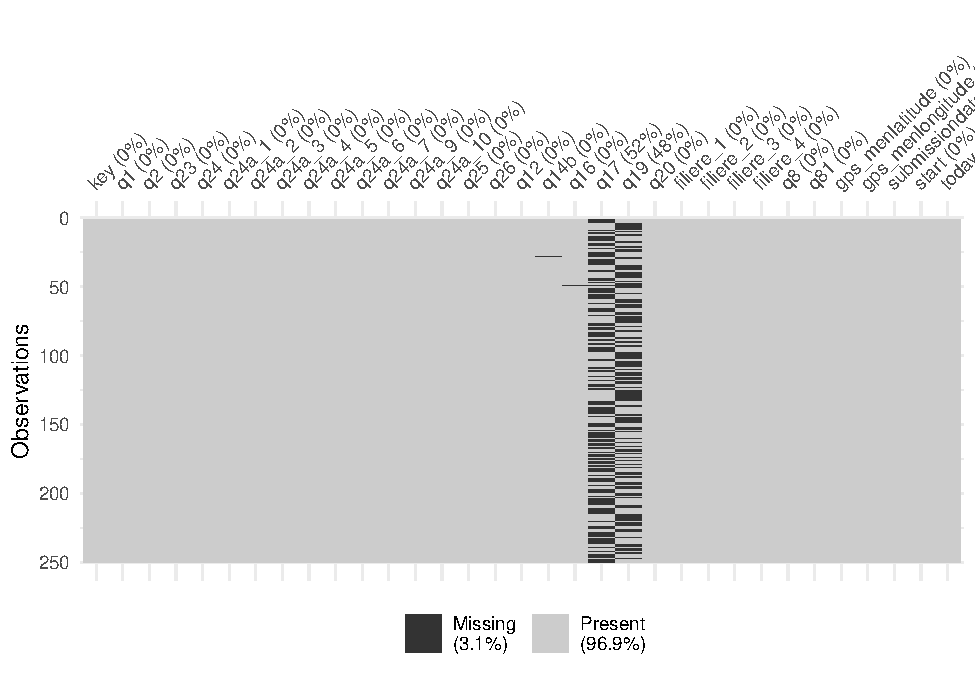
\includegraphics{PROJET_files/figure-latex/unnamed-chunk-5-1.pdf}

\begin{Shaded}
\begin{Highlighting}[]
\CommentTok{\#}
\end{Highlighting}
\end{Shaded}

\newpage

\textcolor{blue}{\subsection{Vérification des valeurs manquantes pour la variable key dans la base projet. Si oui, identifi la (ou les)
PME concernée(s).}}

\begin{Shaded}
\begin{Highlighting}[]
\CommentTok{\#{-}{-}{-}{-}{-}{-}{-}{-}{-}{-}{-}{-}{-}{-}{-}{-}{-}{-}{-}{-}{-}{-}{-}{-}{-}{-}{-}{-}{-}{-}{-}{-}{-}{-}{-}{-}{-}{-}{-}{-}{-}{-}{-}{-}{-}{-}{-}{-}{-}{-}{-}{-}{-}{-}{-}{-}{-}{-}{-}{-}{-}{-}{-}{-}{-}{-}{-}{-}{-}{-}{-}{-}{-}{-}{-}{-}{-}{-}{-}{-}{-}{-}{-}{-}{-}{-}{-}{-}{-}{-}{-}}
\CommentTok{\#       Filtrer les lignes où la colonne "key"                }
\CommentTok{\#     contient des valeurs manquantes (NA)                    }
\CommentTok{\#{-}{-}{-}{-}{-}{-}{-}{-}{-}{-}{-}{-}{-}{-}{-}{-}{-}{-}{-}{-}{-}{-}{-}{-}{-}{-}{-}{-}{-}{-}{-}{-}{-}{-}{-}{-}{-}{-}{-}{-}{-}{-}{-}{-}{-}{-}{-}{-}{-}{-}{-}{-}{-}{-}{-}{-}{-}{-}{-}{-}{-}{-}{-}{-}{-}{-}{-}{-}{-}{-}{-}{-}{-}{-}{-}{-}{-}{-}{-}{-}{-}{-}{-}{-}{-}{-}{-}{-}{-}{-}{-}}

\NormalTok{projet }\SpecialCharTok{\%\textgreater{}\%}
  
\FunctionTok{filter}\NormalTok{(}\FunctionTok{is.na}\NormalTok{(key))}
\end{Highlighting}
\end{Shaded}

\begin{verbatim}
## # A tibble: 0 x 33
## # i 33 variables: key <chr>, q1 <chr>, q2 <chr>, q23 <chr>, q24 <dbl>,
## #   q24a_1 <dbl>, q24a_2 <dbl>, q24a_3 <dbl>, q24a_4 <dbl>, q24a_5 <dbl>,
## #   q24a_6 <dbl>, q24a_7 <dbl>, q24a_9 <dbl>, q24a_10 <dbl>, q25 <chr>,
## #   q26 <dbl>, q12 <chr>, q14b <chr>, q16 <chr>, q17 <chr>, q19 <chr>,
## #   q20 <chr>, filiere_1 <dbl>, filiere_2 <dbl>, filiere_3 <dbl>,
## #   filiere_4 <dbl>, q8 <chr>, q81 <chr>, gps_menlatitude <dbl>,
## #   gps_menlongitude <dbl>, submissiondate <dttm>, start <dttm>, ...
\end{verbatim}

\begin{Shaded}
\begin{Highlighting}[]
\CommentTok{\#}
\end{Highlighting}
\end{Shaded}

\textcolor{blue}{\subsection{Création de variables}}

\textcolor{blue}{\subsection{Nomination de quelques variables}}

\begin{Shaded}
\begin{Highlighting}[]
\CommentTok{\#{-}{-}{-}{-}{-}{-}{-}{-}{-}{-}{-}{-}{-}{-}{-}{-}{-}{-}{-}{-}{-}{-}{-}{-}{-}{-}{-}{-}{-}{-}{-}{-}{-}{-}{-}{-}{-}{-}{-}{-}{-}{-}{-}{-}{-}{-}{-}{-}{-}{-}{-}{-}{-}{-}{-}{-}{-}{-}{-}{-}{-}{-}{-}{-}{-}{-}{-}{-}{-}{-}{-}{-}{-}{-}{-}{-}{-}{-}{-}{-}{-}{-}{-}{-}{-}{-}{-}{-}{-}{-}}
\CommentTok{\#     La fonction rename() est utilisée pour renommer         }
\CommentTok{\#           les colonnes du dataframe.                        }
\CommentTok{\#{-}{-}{-}{-}{-}{-}{-}{-}{-}{-}{-}{-}{-}{-}{-}{-}{-}{-}{-}{-}{-}{-}{-}{-}{-}{-}{-}{-}{-}{-}{-}{-}{-}{-}{-}{-}{-}{-}{-}{-}{-}{-}{-}{-}{-}{-}{-}{-}{-}{-}{-}{-}{-}{-}{-}{-}{-}{-}{-}{-}{-}{-}{-}{-}{-}{-}{-}{-}{-}{-}{-}{-}{-}{-}{-}{-}{-}{-}{-}{-}{-}{-}{-}{-}{-}{-}{-}{-}{-}{-}}

\NormalTok{projet }\OtherTok{\textless{}{-}}\NormalTok{ projet }\SpecialCharTok{\%\textgreater{}\%}
  
  \FunctionTok{rename}\NormalTok{(}
    
    \AttributeTok{region =}\NormalTok{ q1,}
         
       \AttributeTok{departement =}\NormalTok{ q2,}
       
       \AttributeTok{sexe =}\NormalTok{ q23}
\NormalTok{    )}

\CommentTok{\#{-}{-}{-}{-}{-}{-}{-}{-}{-}{-}{-}{-}{-}{-}{-}{-}{-}{-}{-}{-}{-}{-}{-}{-}{-}{-}{-}{-}{-}{-}{-}{-}{-}{-}{-}{-}{-}{-}{-}{-}{-}{-}{-}{-}{-}{-}{-}{-}{-}{-}{-}{-}{-}{-}{-}{-}{-}{-}{-}{-}{-}{-}{-}{-}{-}{-}{-}{-}{-}{-}{-}{-}{-}{-}{-}{-}{-}{-}{-}{-}{-}{-}{-}{-}{-}{-}{-}{-}{-}{-}{-}}
\CommentTok{\#     Afficher les colonnes pour verification}
\CommentTok{\#{-}{-}{-}{-}{-}{-}{-}{-}{-}{-}{-}{-}{-}{-}{-}{-}{-}{-}{-}{-}{-}{-}{-}{-}{-}{-}{-}{-}{-}{-}{-}{-}{-}{-}{-}{-}{-}{-}{-}{-}{-}{-}{-}{-}{-}{-}{-}{-}{-}{-}{-}{-}{-}{-}{-}{-}{-}{-}{-}{-}{-}{-}{-}{-}{-}{-}{-}{-}{-}{-}{-}{-}{-}{-}{-}{-}{-}{-}{-}{-}{-}{-}{-}{-}{-}{-}{-}{-}{-}{-}}

\NormalTok{projet }\SpecialCharTok{\%\textgreater{}\%}
  
  \FunctionTok{names}\NormalTok{()}
\end{Highlighting}
\end{Shaded}

\begin{verbatim}
##  [1] "key"              "region"           "departement"      "sexe"            
##  [5] "q24"              "q24a_1"           "q24a_2"           "q24a_3"          
##  [9] "q24a_4"           "q24a_5"           "q24a_6"           "q24a_7"          
## [13] "q24a_9"           "q24a_10"          "q25"              "q26"             
## [17] "q12"              "q14b"             "q16"              "q17"             
## [21] "q19"              "q20"              "filiere_1"        "filiere_2"       
## [25] "filiere_3"        "filiere_4"        "q8"               "q81"             
## [29] "gps_menlatitude"  "gps_menlongitude" "submissiondate"   "start"           
## [33] "today"
\end{verbatim}

\begin{Shaded}
\begin{Highlighting}[]
\CommentTok{\#}
\end{Highlighting}
\end{Shaded}

\newpage

\textcolor{blue}{\subsection{Création de la variable sexe\_2 qui vaut 1 si sexe égale à Femme et 0 sinon}}

\begin{Shaded}
\begin{Highlighting}[]
\CommentTok{\#{-}{-}{-}{-}{-}{-}{-}{-}{-}{-}{-}{-}{-}{-}{-}{-}{-}{-}{-}{-}{-}{-}{-}{-}{-}{-}{-}{-}{-}{-}{-}{-}{-}{-}{-}{-}{-}{-}{-}{-}{-}{-}{-}{-}{-}{-}{-}{-}{-}{-}{-}{-}{-}{-}{-}{-}{-}{-}{-}{-}{-}{-}{-}{-}{-}{-}{-}{-}{-}{-}{-}{-}{-}{-}{-}{-}{-}{-}{-}{-}{-}{-}{-}{-}{-}{-}{-}{-}{-}}
\CommentTok{\#     la fonction "mutate()" du package dplyr pour ajouter }
\CommentTok{\#         une nouvelle colonne nommée "sexe\_2" avec }
\CommentTok{\#   la condition ifelse(). Si la valeur de la colonne "sexe"  }
\CommentTok{\#     est égale à "Homme", alors la valeur de la colonne }
\CommentTok{\#           "sexe\_2" sera 0, sinon elle sera 1}
\CommentTok{\#{-}{-}{-}{-}{-}{-}{-}{-}{-}{-}{-}{-}{-}{-}{-}{-}{-}{-}{-}{-}{-}{-}{-}{-}{-}{-}{-}{-}{-}{-}{-}{-}{-}{-}{-}{-}{-}{-}{-}{-}{-}{-}{-}{-}{-}{-}{-}{-}{-}{-}{-}{-}{-}{-}{-}{-}{-}{-}{-}{-}{-}{-}{-}{-}{-}{-}{-}{-}{-}{-}{-}{-}{-}{-}{-}{-}{-}{-}{-}{-}{-}{-}{-}{-}{-}{-}{-}{-}{-}}

\NormalTok{projet }\OtherTok{\textless{}{-}}\NormalTok{ projet }\SpecialCharTok{\%\textgreater{}\%}
  
\NormalTok{  dplyr}\SpecialCharTok{::}\FunctionTok{mutate}\NormalTok{(}\AttributeTok{sexe\_2 =} \FunctionTok{ifelse}\NormalTok{(sexe }\SpecialCharTok{==} \StringTok{"Homme"}\NormalTok{, }\DecValTok{0}\NormalTok{, }\DecValTok{1}\NormalTok{), }\AttributeTok{.after =}
\NormalTok{sexe)}


\CommentTok{\#{-}{-}{-}{-}{-}{-}{-}{-}{-}{-}{-}{-}{-}{-}{-}{-}{-}{-}{-}{-}{-}{-}{-}{-}{-}{-}{-}{-}{-}{-}{-}{-}{-}{-}{-}{-}{-}{-}{-}{-}{-}{-}{-}{-}{-}{-}{-}{-}{-}{-}{-}{-}{-}{-}{-}{-}{-}{-}{-}{-}{-}{-}{-}{-}{-}{-}{-}{-}{-}{-}{-}{-}{-}{-}{-}{-}{-}{-}{-}{-}{-}{-}{-}{-}{-}{-}{-}{-}}
\CommentTok{\#     Afficher les colonnes pour verification}
\CommentTok{\#{-}{-}{-}{-}{-}{-}{-}{-}{-}{-}{-}{-}{-}{-}{-}{-}{-}{-}{-}{-}{-}{-}{-}{-}{-}{-}{-}{-}{-}{-}{-}{-}{-}{-}{-}{-}{-}{-}{-}{-}{-}{-}{-}{-}{-}{-}{-}{-}{-}{-}{-}{-}{-}{-}{-}{-}{-}{-}{-}{-}{-}{-}{-}{-}{-}{-}{-}{-}{-}{-}{-}{-}{-}{-}{-}{-}{-}{-}{-}{-}{-}{-}{-}{-}{-}{-}{-}{-}}

\NormalTok{projet }\SpecialCharTok{\%\textgreater{}\%}
  
  \FunctionTok{head}\NormalTok{()}
\end{Highlighting}
\end{Shaded}

\begin{verbatim}
## # A tibble: 6 x 34
##   key   region departement sexe  sexe_2   q24 q24a_1 q24a_2 q24a_3 q24a_4 q24a_5
##   <chr> <chr>  <chr>       <chr>  <dbl> <dbl>  <dbl>  <dbl>  <dbl>  <dbl>  <dbl>
## 1 uuid~ Diour~ Bambey      Femme      1    65      0      1      0      1      0
## 2 uuid~ Thiès  Mbour       Femme      1    52      1      1      0      0      1
## 3 uuid~ Thiès  Mbour       Femme      1    65      1      1      0      0      0
## 4 uuid~ Thiès  Mbour       Femme      1    38      1      1      0      0      1
## 5 uuid~ Zigui~ Bignona     Homme      0    40      1      1      1      0      0
## 6 uuid~ Zigui~ Oussouye    Femme      1    43      1      1      1      0      0
## # i 23 more variables: q24a_6 <dbl>, q24a_7 <dbl>, q24a_9 <dbl>, q24a_10 <dbl>,
## #   q25 <chr>, q26 <dbl>, q12 <chr>, q14b <chr>, q16 <chr>, q17 <chr>,
## #   q19 <chr>, q20 <chr>, filiere_1 <dbl>, filiere_2 <dbl>, filiere_3 <dbl>,
## #   filiere_4 <dbl>, q8 <chr>, q81 <chr>, gps_menlatitude <dbl>,
## #   gps_menlongitude <dbl>, submissiondate <dttm>, start <dttm>, today <dttm>
\end{verbatim}

\begin{Shaded}
\begin{Highlighting}[]
\CommentTok{\#}
\end{Highlighting}
\end{Shaded}

\textcolor{blue}{\subsection{Création d’un data.frame nommé langues qui prend les variables key et les variables correspondantes}}

\begin{Shaded}
\begin{Highlighting}[]
\CommentTok{\#{-}{-}{-}{-}{-}{-}{-}{-}{-}{-}{-}{-}{-}{-}{-}{-}{-}{-}{-}{-}{-}{-}{-}{-}{-}{-}{-}{-}{-}{-}{-}{-}{-}{-}{-}{-}{-}{-}{-}{-}{-}{-}{-}{-}{-}{-}{-}{-}{-}{-}{-}{-}{-}{-}{-}{-}{-}{-}{-}{-}{-}{-}{-}{-}{-}{-}{-}{-}{-}{-}{-}{-}{-}{-}{-}{-}{-}{-}{-}{-}{-}{-}{-}{-}{-}{-}{-}{-}{-}{-}}
\CommentTok{\#     Selection a partie la fonction "select()" de dplyr :}
\CommentTok{\#       la colonne "key" et toutes les variables commençant }
\CommentTok{\#             par q24a\_ "starts\_with(q24a\_)"  }
\CommentTok{\#{-}{-}{-}{-}{-}{-}{-}{-}{-}{-}{-}{-}{-}{-}{-}{-}{-}{-}{-}{-}{-}{-}{-}{-}{-}{-}{-}{-}{-}{-}{-}{-}{-}{-}{-}{-}{-}{-}{-}{-}{-}{-}{-}{-}{-}{-}{-}{-}{-}{-}{-}{-}{-}{-}{-}{-}{-}{-}{-}{-}{-}{-}{-}{-}{-}{-}{-}{-}{-}{-}{-}{-}{-}{-}{-}{-}{-}{-}{-}{-}{-}{-}{-}{-}{-}{-}{-}{-}{-}{-}}

\NormalTok{langues }\OtherTok{\textless{}{-}}\NormalTok{ projet }\SpecialCharTok{\%\textgreater{}\%}
  
\NormalTok{  dplyr}\SpecialCharTok{::}\FunctionTok{select}\NormalTok{(key,}\FunctionTok{starts\_with}\NormalTok{(}\StringTok{"q24a\_"}\NormalTok{))}


\CommentTok{\#{-}{-}{-}{-}{-}{-}{-}{-}{-}{-}{-}{-}{-}{-}{-}{-}{-}{-}{-}{-}{-}{-}{-}{-}{-}{-}{-}{-}{-}{-}{-}{-}{-}{-}{-}{-}{-}{-}{-}{-}{-}{-}{-}{-}{-}{-}{-}{-}{-}{-}{-}{-}{-}{-}{-}{-}{-}{-}{-}{-}{-}{-}{-}{-}{-}{-}{-}{-}{-}{-}{-}{-}{-}{-}{-}{-}{-}{-}{-}{-}{-}{-}{-}{-}{-}{-}}
\CommentTok{\#     Afficher les colonnes pour verification}
\CommentTok{\#{-}{-}{-}{-}{-}{-}{-}{-}{-}{-}{-}{-}{-}{-}{-}{-}{-}{-}{-}{-}{-}{-}{-}{-}{-}{-}{-}{-}{-}{-}{-}{-}{-}{-}{-}{-}{-}{-}{-}{-}{-}{-}{-}{-}{-}{-}{-}{-}{-}{-}{-}{-}{-}{-}{-}{-}{-}{-}{-}{-}{-}{-}{-}{-}{-}{-}{-}{-}{-}{-}{-}{-}{-}{-}{-}{-}{-}{-}{-}{-}{-}{-}{-}{-}{-}{-}}

\NormalTok{langues }\SpecialCharTok{\%\textgreater{}\%}
  
  \FunctionTok{head}\NormalTok{()}
\end{Highlighting}
\end{Shaded}

\begin{verbatim}
## # A tibble: 6 x 10
##   key            q24a_1 q24a_2 q24a_3 q24a_4 q24a_5 q24a_6 q24a_7 q24a_9 q24a_10
##   <chr>           <dbl>  <dbl>  <dbl>  <dbl>  <dbl>  <dbl>  <dbl>  <dbl>   <dbl>
## 1 uuid:68bff42b~      0      1      0      1      0      0      0      0       0
## 2 uuid:d70b3c7e~      1      1      0      0      1      0      0      0       0
## 3 uuid:0ac18b64~      1      1      0      0      0      0      0      0       0
## 4 uuid:c52cf5e4~      1      1      0      0      1      0      0      0       0
## 5 uuid:ac177870~      1      1      1      0      0      1      0      0       0
## 6 uuid:578097cf~      1      1      1      0      0      0      0      0       0
\end{verbatim}

\begin{Shaded}
\begin{Highlighting}[]
\CommentTok{\#}
\end{Highlighting}
\end{Shaded}

\textcolor{blue}{\subsection{Création de la variable “parle” qui est égale au nombre de langue parlée par le dirigeant de la PME}}

\begin{Shaded}
\begin{Highlighting}[]
\CommentTok{\# {-}{-}{-}{-}{-}{-}{-}{-}{-}{-}{-}{-}{-}{-}{-}{-}{-}{-}{-}{-}{-}{-}{-}{-}{-}{-}{-}{-}{-}{-}{-}{-}{-}{-}{-}{-}{-}{-}{-}{-}{-}{-}{-}{-}{-}{-}{-}{-}{-}{-}{-}{-}{-}{-}{-}{-}{-}{-}{-}{-}{-}{-}{-}{-}{-}{-}{-}{-}{-}{-}{-}{-}{-}{-}{-}{-}{-}{-}{-}{-}{-}{-}{-}{-}{-}{-}{-}{-}}
\CommentTok{\#    Sommer par ligne avec rowSums() les lignes donc }
\CommentTok{\#      les langues prennent la valeur = 1 et selectionner}
\CommentTok{\#          directement avec transmute() key et }
\CommentTok{\#               la nouvellevariable}
\CommentTok{\#{-}{-}{-}{-}{-}{-}{-}{-}{-}{-}{-}{-}{-}{-}{-}{-}{-}{-}{-}{-}{-}{-}{-}{-}{-}{-}{-}{-}{-}{-}{-}{-}{-}{-}{-}{-}{-}{-}{-}{-}{-}{-}{-}{-}{-}{-}{-}{-}{-}{-}{-}{-}{-}{-}{-}{-}{-}{-}{-}{-}{-}{-}{-}{-}{-}{-}{-}{-}{-}{-}{-}{-}{-}{-}{-}{-}{-}{-}{-}{-}{-}{-}{-}{-}{-}{-}{-}{-}{-}{-}}

\NormalTok{nombre\_langue }\OtherTok{\textless{}{-}}\NormalTok{ projet }\SpecialCharTok{\%\textgreater{}\%}
  
  \FunctionTok{transmute}\NormalTok{(key,}\AttributeTok{parle =} \FunctionTok{rowSums}\NormalTok{(langues }\SpecialCharTok{==} \StringTok{"1"}\NormalTok{) )}


\CommentTok{\#{-}{-}{-}{-}{-}{-}{-}{-}{-}{-}{-}{-}{-}{-}{-}{-}{-}{-}{-}{-}{-}{-}{-}{-}{-}{-}{-}{-}{-}{-}{-}{-}{-}{-}{-}{-}{-}{-}{-}{-}{-}{-}{-}{-}{-}{-}{-}{-}{-}{-}{-}{-}{-}{-}{-}{-}{-}{-}{-}{-}{-}{-}{-}{-}{-}{-}{-}{-}{-}{-}{-}{-}{-}{-}{-}{-}{-}{-}{-}{-}{-}{-}{-}{-}{-}{-}{-}{-}{-}}
\CommentTok{\#     Afficher les colonnes pour verification}
\CommentTok{\#{-}{-}{-}{-}{-}{-}{-}{-}{-}{-}{-}{-}{-}{-}{-}{-}{-}{-}{-}{-}{-}{-}{-}{-}{-}{-}{-}{-}{-}{-}{-}{-}{-}{-}{-}{-}{-}{-}{-}{-}{-}{-}{-}{-}{-}{-}{-}{-}{-}{-}{-}{-}{-}{-}{-}{-}{-}{-}{-}{-}{-}{-}{-}{-}{-}{-}{-}{-}{-}{-}{-}{-}{-}{-}{-}{-}{-}{-}{-}{-}{-}{-}{-}{-}{-}{-}{-}{-}{-}}

\NormalTok{nombre\_langue }\SpecialCharTok{\%\textgreater{}\%}
  
  \FunctionTok{head}\NormalTok{()}\SpecialCharTok{\%\textgreater{}\%} 
  
  \FunctionTok{gt}\NormalTok{()}
\end{Highlighting}
\end{Shaded}

\begin{longtable}{lr}
\toprule
key & parle \\ 
\midrule
uuid:68bff42b-1228-4c66-9bcc-e6d312d9fea6 & 2 \\ 
uuid:d70b3c7e-3ca0-4358-bc59-3f7f6baf55e9 & 3 \\ 
uuid:0ac18b64-7d85-4bb9-a842-698ac79909af & 2 \\ 
uuid:c52cf5e4-8c28-4e65-998b-3fe2a971a1a3 & 3 \\ 
uuid:ac177870-001c-4ada-8747-c22ffe4e4596 & 4 \\ 
uuid:578097cf-9af7-46e6-8992-d9079b14c342 & 3 \\ 
\bottomrule
\end{longtable}

\begin{Shaded}
\begin{Highlighting}[]
\CommentTok{\#}
\end{Highlighting}
\end{Shaded}

\textcolor{blue}{\subsection{Fusion de data.frame projet et langues}}

\begin{Shaded}
\begin{Highlighting}[]
\CommentTok{\#{-}{-}{-}{-}{-}{-}{-}{-}{-}{-}{-}{-}{-}{-}{-}{-}{-}{-}{-}{-}{-}{-}{-}{-}{-}{-}{-}{-}{-}{-}{-}{-}{-}{-}{-}{-}{-}{-}{-}{-}{-}{-}{-}{-}{-}{-}{-}{-}{-}{-}{-}{-}{-}{-}{-}{-}{-}{-}{-}{-}{-}{-}{-}{-}{-}{-}{-}{-}{-}{-}{-}{-}{-}{-}{-}{-}{-}{-}{-}{-}{-}{-}{-}{-}{-}{-}{-}{-}}
\CommentTok{\#   fusion des dataframes "projet" et "langues" en utilisant}
\CommentTok{\#          la colonne "key" comme clé de fusion}
\CommentTok{\#              avec la fonction  "merge()" de base en R}
\CommentTok{\#{-}{-}{-}{-}{-}{-}{-}{-}{-}{-}{-}{-}{-}{-}{-}{-}{-}{-}{-}{-}{-}{-}{-}{-}{-}{-}{-}{-}{-}{-}{-}{-}{-}{-}{-}{-}{-}{-}{-}{-}{-}{-}{-}{-}{-}{-}{-}{-}{-}{-}{-}{-}{-}{-}{-}{-}{-}{-}{-}{-}{-}{-}{-}{-}{-}{-}{-}{-}{-}{-}{-}{-}{-}{-}{-}{-}{-}{-}{-}{-}{-}{-}{-}{-}{-}{-}{-}{-}}

\NormalTok{fusion }\OtherTok{=} \FunctionTok{merge}\NormalTok{(projet,langues, }\AttributeTok{by =} \StringTok{"key"}\NormalTok{)}

\CommentTok{\#}
\end{Highlighting}
\end{Shaded}

\newpage

\textcolor{blue}{\subsection{Analyses descriptives}}

\textcolor{blue}{\subsection{La répartion des PME}}

\begin{Shaded}
\begin{Highlighting}[]
\CommentTok{\#{-}{-}{-}{-}{-}{-}{-}{-}{-}{-}{-}{-}{-}{-}{-}{-}{-}{-}{-}{-}{-}{-}{-}{-}{-}{-}{-}{-}{-}{-}{-}{-}{-}{-}{-}{-}{-}{-}{-}{-}{-}{-}{-}{-}{-}{-}{-}{-}{-}{-}{-}{-}{-}{-}{-}{-}{-}{-}{-}{-}{-}{-}{-}{-}{-}{-}{-}{-}{-}{-}{-}{-}{-}{-}{-}{-}{-}{-}{-}{-}{-}{-}{-}{-}{-}{-}{-}{-}}
\CommentTok{\#         Personnaliser les paramètres de langue pour}
\CommentTok{\#   le français (fr) dans les tables générées par gtsummary}
\CommentTok{\#{-}{-}{-}{-}{-}{-}{-}{-}{-}{-}{-}{-}{-}{-}{-}{-}{-}{-}{-}{-}{-}{-}{-}{-}{-}{-}{-}{-}{-}{-}{-}{-}{-}{-}{-}{-}{-}{-}{-}{-}{-}{-}{-}{-}{-}{-}{-}{-}{-}{-}{-}{-}{-}{-}{-}{-}{-}{-}{-}{-}{-}{-}{-}{-}{-}{-}{-}{-}{-}{-}{-}{-}{-}{-}{-}{-}{-}{-}{-}{-}{-}{-}{-}{-}{-}{-}{-}{-}}



\FunctionTok{theme\_gtsummary\_language}\NormalTok{(}\StringTok{"fr"}\NormalTok{,}\AttributeTok{decimal.mark =} \StringTok{","}\NormalTok{, }\AttributeTok{big.mark =}\StringTok{" "}\NormalTok{)}




\CommentTok{\#{-}{-}{-}{-}{-}{-}{-}{-}{-}{-}{-}{-}{-}{-}{-}{-}{-}{-}{-}{-}{-}{-}{-}{-}{-}{-}{-}{-}{-}{-}{-}{-}{-}{-}{-}{-}{-}{-}{-}{-}{-}{-}{-}{-}{-}{-}{-}{-}{-}{-}{-}{-}{-}{-}{-}{-}{-}{-}{-}{-}{-}{-}{-}{-}{-}{-}{-}{-}{-}{-}{-}{-}{-}{-}{-}{-}{-}{-}{-}{-}{-}{-}{-}{-}{-}{-}{-}{-}}
\CommentTok{\#  La fonction tbl\_summary() du package gtsummary }
\CommentTok{\#   utilisée pour créer le tableau de résumé des colonnes}
\CommentTok{\#     "SEXE" , "NIVEAU D’INSTRUCTION","STATUT JURIDIQUE"}
\CommentTok{\#        et "PROPRIETAIRE/LOCATAIRE"}
\CommentTok{\#{-}{-}{-}{-}{-}{-}{-}{-}{-}{-}{-}{-}{-}{-}{-}{-}{-}{-}{-}{-}{-}{-}{-}{-}{-}{-}{-}{-}{-}{-}{-}{-}{-}{-}{-}{-}{-}{-}{-}{-}{-}{-}{-}{-}{-}{-}{-}{-}{-}{-}{-}{-}{-}{-}{-}{-}{-}{-}{-}{-}{-}{-}{-}{-}{-}{-}{-}{-}{-}{-}{-}{-}{-}{-}{-}{-}{-}{-}{-}{-}{-}{-}{-}{-}{-}{-}{-}{-}}




\NormalTok{tab1 }\OtherTok{=}\NormalTok{ projet }\SpecialCharTok{\%\textgreater{}\%}
  
  
\NormalTok{  gtsummary}\SpecialCharTok{::}\FunctionTok{tbl\_summary}\NormalTok{(}
    
    \AttributeTok{include =} \FunctionTok{c}\NormalTok{(}\StringTok{"sexe"}\NormalTok{,}\StringTok{"q25"}\NormalTok{,}\StringTok{"q12"}\NormalTok{,}\StringTok{"q81"}\NormalTok{),}
    
    \AttributeTok{statistic =}  \FunctionTok{list}\NormalTok{( }\FunctionTok{all\_categorical}\NormalTok{() }\SpecialCharTok{\textasciitilde{}} \StringTok{"\{p\}\% (\{n\}/\{N\})"}\NormalTok{),}
    
    \AttributeTok{label =} \FunctionTok{list}\NormalTok{( q25 }\SpecialCharTok{\textasciitilde{}} \StringTok{"NIVEAU D’INSTRUCTION"}\NormalTok{,}
                  
\NormalTok{                  q12 }\SpecialCharTok{\textasciitilde{}} \StringTok{"STATUT JURIDIQUE"}\NormalTok{,}
                  
\NormalTok{                  q81 }\SpecialCharTok{\textasciitilde{}} \StringTok{"PROPRIETAIRE/LOCATAIRE"}\NormalTok{,}
                  
\NormalTok{                  sexe }\SpecialCharTok{\textasciitilde{}} \StringTok{"SEXE"} 
\NormalTok{                  )}
\NormalTok{  )}


\CommentTok{\#{-}{-}{-}{-}{-}{-}{-}{-}{-}{-}{-}{-}{-}{-}{-}{-}{-}{-}{-}{-}{-}{-}{-}{-}{-}{-}{-}{-}{-}{-}{-}{-}{-}{-}{-}{-}{-}{-}{-}{-}{-}{-}{-}{-}{-}{-}{-}{-}{-}{-}{-}{-}{-}{-}{-}{-}{-}{-}{-}{-}{-}{-}{-}{-}{-}{-}{-}{-}{-}{-}{-}{-}{-}{-}{-}{-}{-}{-}{-}{-}{-}{-}{-}{-}{-}{-}{-}{-}{-}{-}}
\CommentTok{\#   Ajout de l\textquotesingle{}option supplémentaire by = sexe pour grouper}
\CommentTok{\#       les statistiques par la variable "sexe" : croisement}
\CommentTok{\#{-}{-}{-}{-}{-}{-}{-}{-}{-}{-}{-}{-}{-}{-}{-}{-}{-}{-}{-}{-}{-}{-}{-}{-}{-}{-}{-}{-}{-}{-}{-}{-}{-}{-}{-}{-}{-}{-}{-}{-}{-}{-}{-}{-}{-}{-}{-}{-}{-}{-}{-}{-}{-}{-}{-}{-}{-}{-}{-}{-}{-}{-}{-}{-}{-}{-}{-}{-}{-}{-}{-}{-}{-}{-}{-}{-}{-}{-}{-}{-}{-}{-}{-}{-}{-}{-}{-}{-}{-}}



\NormalTok{tab2 }\OtherTok{=}\NormalTok{ projet }\SpecialCharTok{\%\textgreater{}\%}
  
  
\NormalTok{  gtsummary}\SpecialCharTok{::}\FunctionTok{tbl\_summary}\NormalTok{(}
    
    \AttributeTok{include =} \FunctionTok{c}\NormalTok{(}\StringTok{"sexe"}\NormalTok{,}\StringTok{"q25"}\NormalTok{,}\StringTok{"q12"}\NormalTok{,}\StringTok{"q81"}\NormalTok{),}
    
    \AttributeTok{by =}\NormalTok{ sexe,}
    
    \AttributeTok{statistic =}  \FunctionTok{list}\NormalTok{( }\FunctionTok{all\_categorical}\NormalTok{() }\SpecialCharTok{\textasciitilde{}} \StringTok{"\{p\}\% (\{n\}/\{N\})"}\NormalTok{),}
    
    \AttributeTok{label =} \FunctionTok{list}\NormalTok{( q25 }\SpecialCharTok{\textasciitilde{}} \StringTok{"NIVEAU D’INSTRUCTION"}\NormalTok{,}
                  
\NormalTok{                  q12 }\SpecialCharTok{\textasciitilde{}} \StringTok{"STATUT JURIDIQUE"}\NormalTok{,}
                  
\NormalTok{                  q81 }\SpecialCharTok{\textasciitilde{}} \StringTok{"PROPRIETAIRE/LOCATAIRE"}\NormalTok{)}
\NormalTok{  )}



\CommentTok{\# {-}{-}{-}{-}{-}{-}{-}{-}{-}{-}{-}{-}{-}{-}{-}{-}{-}{-}{-}{-}{-}{-}{-}{-}{-}{-}{-}{-}{-}{-}{-}{-}{-}{-}{-}{-}{-}{-}{-}{-}{-}{-}{-}{-}{-}{-}{-}{-}{-}{-}{-}{-}{-}{-}{-}{-}{-}{-}{-}{-}{-}{-}{-}{-}{-}{-}{-}{-}{-}{-}{-}{-}{-}{-}{-}{-}{-}{-}{-}{-}{-}{-}{-}{-}{-}{-}{-}{-}}
\CommentTok{\# la fonction tbl\_merge() du package gtsummary pour fusionner}
\CommentTok{\#  les deux tableaux de résumé tab1 et tab2 créés précédemment}
\CommentTok{\#{-}{-}{-}{-}{-}{-}{-}{-}{-}{-}{-}{-}{-}{-}{-}{-}{-}{-}{-}{-}{-}{-}{-}{-}{-}{-}{-}{-}{-}{-}{-}{-}{-}{-}{-}{-}{-}{-}{-}{-}{-}{-}{-}{-}{-}{-}{-}{-}{-}{-}{-}{-}{-}{-}{-}{-}{-}{-}{-}{-}{-}{-}{-}{-}{-}{-}{-}{-}{-}{-}{-}{-}{-}{-}{-}{-}{-}{-}{-}{-}{-}{-}{-}{-}{-}{-}{-}{-}{-}}



\FunctionTok{tbl\_merge}\NormalTok{(}\FunctionTok{list}\NormalTok{(tab1,tab2),}\AttributeTok{tab\_spanner =} \FunctionTok{c}\NormalTok{(}\StringTok{"ANALYSE UNIVARIE"}\NormalTok{,}\StringTok{"ANALYSE BIVARIE"}\NormalTok{))}\SpecialCharTok{\%\textgreater{}\%}
  
  
  \FunctionTok{bold\_labels}\NormalTok{() }\SpecialCharTok{\%\textgreater{}\%} 
  
  
  \FunctionTok{italicize\_levels}\NormalTok{()  }\SpecialCharTok{\%\textgreater{}\%} 
  
  
  \FunctionTok{modify\_header}\NormalTok{(}
    \AttributeTok{update =} \FunctionTok{list}\NormalTok{( label }\SpecialCharTok{\textasciitilde{}} \StringTok{"**VARIABLE**"}\NormalTok{,}
                   \FunctionTok{all\_stat\_cols}\NormalTok{(}\AttributeTok{stat\_0 =} \ConstantTok{FALSE}\NormalTok{) }\SpecialCharTok{\textasciitilde{}} \StringTok{"**\{level\}** (n=\{n\}, \{style\_percent(p)\}\%)"}
\NormalTok{  )) }\SpecialCharTok{\%\textgreater{}\%} 
  
  
  \FunctionTok{as\_flex\_table}\NormalTok{() }\SpecialCharTok{\%\textgreater{}\%}
  
  
  \FunctionTok{fontsize}\NormalTok{(}\AttributeTok{size =} \DecValTok{8}\NormalTok{) }\SpecialCharTok{\%\textgreater{}\%}
  
  
  \FunctionTok{width}\NormalTok{(}\AttributeTok{width =} \FloatTok{1.65}\NormalTok{)}
\end{Highlighting}
\end{Shaded}

\global\setlength{\Oldarrayrulewidth}{\arrayrulewidth}

\global\setlength{\Oldtabcolsep}{\tabcolsep}

\setlength{\tabcolsep}{0pt}

\renewcommand*{\arraystretch}{1.5}



\providecommand{\ascline}[3]{\noalign{\global\arrayrulewidth #1}\arrayrulecolor[HTML]{#2}\cline{#3}}

\begin{longtable}[c]{|p{1.65in}|p{1.65in}|p{1.65in}|p{1.65in}}



\ascline{1pt}{000000}{1-4}

\multicolumn{1}{>{\raggedright}m{\dimexpr 1.65in+0\tabcolsep}}{\textcolor[HTML]{000000}{\fontsize{11}{11}\selectfont{\ }}} & \multicolumn{1}{>{\centering}m{\dimexpr 1.65in+0\tabcolsep}}{\textcolor[HTML]{000000}{\fontsize{11}{11}\selectfont{ANALYSE\ UNIVARIE}}} & \multicolumn{2}{>{\centering}m{\dimexpr 3.3in+2\tabcolsep}}{\textcolor[HTML]{000000}{\fontsize{11}{11}\selectfont{ANALYSE\ BIVARIE}}} \\

\ascline{1pt}{000000}{1-4}



\multicolumn{1}{>{\raggedright}m{\dimexpr 1.65in+0\tabcolsep}}{\textcolor[HTML]{000000}{\fontsize{11}{11}\selectfont{\textbf{VARIABLE}}}} & \multicolumn{1}{>{\centering}m{\dimexpr 1.65in+0\tabcolsep}}{\textcolor[HTML]{000000}{\fontsize{11}{11}\selectfont{\textbf{N\ =\ 250}}}\textcolor[HTML]{000000}{\textsuperscript{\fontsize{11}{11}\selectfont{1}}}} & \multicolumn{1}{>{\centering}m{\dimexpr 1.65in+0\tabcolsep}}{\textcolor[HTML]{000000}{\fontsize{11}{11}\selectfont{\textbf{Femme}}}\textcolor[HTML]{000000}{\fontsize{11}{11}\selectfont{\ (n=191,\ 76\%)}}\textcolor[HTML]{000000}{\textsuperscript{\fontsize{11}{11}\selectfont{1}}}} & \multicolumn{1}{>{\centering}m{\dimexpr 1.65in+0\tabcolsep}}{\textcolor[HTML]{000000}{\fontsize{11}{11}\selectfont{\textbf{Homme}}}\textcolor[HTML]{000000}{\fontsize{11}{11}\selectfont{\ (n=59,\ 24\%)}}\textcolor[HTML]{000000}{\textsuperscript{\fontsize{11}{11}\selectfont{1}}}} \\

\ascline{1pt}{000000}{1-4}\endhead



\multicolumn{4}{>{\raggedright}m{\dimexpr 6.6in+6\tabcolsep}}{\textcolor[HTML]{000000}{\textsuperscript{\fontsize{11}{11}\selectfont{1}}}\textcolor[HTML]{000000}{\fontsize{11}{11}\selectfont{\%\ (n/N)}}} \\

\endfoot



\multicolumn{1}{>{\raggedright}p{\dimexpr 1.65in+0\tabcolsep}}{\textcolor[HTML]{000000}{\fontsize{8}{8}\selectfont{\textbf{SEXE}}}} & \multicolumn{1}{>{\centering}p{\dimexpr 1.65in+0\tabcolsep}}{\textcolor[HTML]{000000}{\fontsize{8}{8}\selectfont{}}} & \multicolumn{1}{>{\centering}p{\dimexpr 1.65in+0\tabcolsep}}{\textcolor[HTML]{000000}{\fontsize{8}{8}\selectfont{}}} & \multicolumn{1}{>{\centering}p{\dimexpr 1.65in+0\tabcolsep}}{\textcolor[HTML]{000000}{\fontsize{8}{8}\selectfont{}}} \\





\multicolumn{1}{>{\raggedright}p{\dimexpr 1.65in+0\tabcolsep}}{\textcolor[HTML]{000000}{\fontsize{8}{8}\selectfont{\textit{Femme}}}} & \multicolumn{1}{>{\centering}p{\dimexpr 1.65in+0\tabcolsep}}{\textcolor[HTML]{000000}{\fontsize{8}{8}\selectfont{76\%\ (191/250)}}} & \multicolumn{1}{>{\centering}p{\dimexpr 1.65in+0\tabcolsep}}{\textcolor[HTML]{000000}{\fontsize{8}{8}\selectfont{}}} & \multicolumn{1}{>{\centering}p{\dimexpr 1.65in+0\tabcolsep}}{\textcolor[HTML]{000000}{\fontsize{8}{8}\selectfont{}}} \\





\multicolumn{1}{>{\raggedright}p{\dimexpr 1.65in+0\tabcolsep}}{\textcolor[HTML]{000000}{\fontsize{8}{8}\selectfont{\textit{Homme}}}} & \multicolumn{1}{>{\centering}p{\dimexpr 1.65in+0\tabcolsep}}{\textcolor[HTML]{000000}{\fontsize{8}{8}\selectfont{24\%\ (59/250)}}} & \multicolumn{1}{>{\centering}p{\dimexpr 1.65in+0\tabcolsep}}{\textcolor[HTML]{000000}{\fontsize{8}{8}\selectfont{}}} & \multicolumn{1}{>{\centering}p{\dimexpr 1.65in+0\tabcolsep}}{\textcolor[HTML]{000000}{\fontsize{8}{8}\selectfont{}}} \\





\multicolumn{1}{>{\raggedright}p{\dimexpr 1.65in+0\tabcolsep}}{\textcolor[HTML]{000000}{\fontsize{8}{8}\selectfont{\textbf{NIVEAU\ D’INSTRUCTION}}}} & \multicolumn{1}{>{\centering}p{\dimexpr 1.65in+0\tabcolsep}}{\textcolor[HTML]{000000}{\fontsize{8}{8}\selectfont{}}} & \multicolumn{1}{>{\centering}p{\dimexpr 1.65in+0\tabcolsep}}{\textcolor[HTML]{000000}{\fontsize{8}{8}\selectfont{}}} & \multicolumn{1}{>{\centering}p{\dimexpr 1.65in+0\tabcolsep}}{\textcolor[HTML]{000000}{\fontsize{8}{8}\selectfont{}}} \\





\multicolumn{1}{>{\raggedright}p{\dimexpr 1.65in+0\tabcolsep}}{\textcolor[HTML]{000000}{\fontsize{8}{8}\selectfont{\textit{Aucun\ niveau}}}} & \multicolumn{1}{>{\centering}p{\dimexpr 1.65in+0\tabcolsep}}{\textcolor[HTML]{000000}{\fontsize{8}{8}\selectfont{32\%\ (79/250)}}} & \multicolumn{1}{>{\centering}p{\dimexpr 1.65in+0\tabcolsep}}{\textcolor[HTML]{000000}{\fontsize{8}{8}\selectfont{37\%\ (70/191)}}} & \multicolumn{1}{>{\centering}p{\dimexpr 1.65in+0\tabcolsep}}{\textcolor[HTML]{000000}{\fontsize{8}{8}\selectfont{15\%\ (9/59)}}} \\





\multicolumn{1}{>{\raggedright}p{\dimexpr 1.65in+0\tabcolsep}}{\textcolor[HTML]{000000}{\fontsize{8}{8}\selectfont{\textit{Niveau\ primaire}}}} & \multicolumn{1}{>{\centering}p{\dimexpr 1.65in+0\tabcolsep}}{\textcolor[HTML]{000000}{\fontsize{8}{8}\selectfont{22\%\ (56/250)}}} & \multicolumn{1}{>{\centering}p{\dimexpr 1.65in+0\tabcolsep}}{\textcolor[HTML]{000000}{\fontsize{8}{8}\selectfont{25\%\ (48/191)}}} & \multicolumn{1}{>{\centering}p{\dimexpr 1.65in+0\tabcolsep}}{\textcolor[HTML]{000000}{\fontsize{8}{8}\selectfont{14\%\ (8/59)}}} \\





\multicolumn{1}{>{\raggedright}p{\dimexpr 1.65in+0\tabcolsep}}{\textcolor[HTML]{000000}{\fontsize{8}{8}\selectfont{\textit{Niveau\ secondaire}}}} & \multicolumn{1}{>{\centering}p{\dimexpr 1.65in+0\tabcolsep}}{\textcolor[HTML]{000000}{\fontsize{8}{8}\selectfont{30\%\ (74/250)}}} & \multicolumn{1}{>{\centering}p{\dimexpr 1.65in+0\tabcolsep}}{\textcolor[HTML]{000000}{\fontsize{8}{8}\selectfont{29\%\ (56/191)}}} & \multicolumn{1}{>{\centering}p{\dimexpr 1.65in+0\tabcolsep}}{\textcolor[HTML]{000000}{\fontsize{8}{8}\selectfont{31\%\ (18/59)}}} \\





\multicolumn{1}{>{\raggedright}p{\dimexpr 1.65in+0\tabcolsep}}{\textcolor[HTML]{000000}{\fontsize{8}{8}\selectfont{\textit{Niveau\ Superieur}}}} & \multicolumn{1}{>{\centering}p{\dimexpr 1.65in+0\tabcolsep}}{\textcolor[HTML]{000000}{\fontsize{8}{8}\selectfont{16\%\ (41/250)}}} & \multicolumn{1}{>{\centering}p{\dimexpr 1.65in+0\tabcolsep}}{\textcolor[HTML]{000000}{\fontsize{8}{8}\selectfont{8,9\%\ (17/191)}}} & \multicolumn{1}{>{\centering}p{\dimexpr 1.65in+0\tabcolsep}}{\textcolor[HTML]{000000}{\fontsize{8}{8}\selectfont{41\%\ (24/59)}}} \\





\multicolumn{1}{>{\raggedright}p{\dimexpr 1.65in+0\tabcolsep}}{\textcolor[HTML]{000000}{\fontsize{8}{8}\selectfont{\textbf{STATUT\ JURIDIQUE}}}} & \multicolumn{1}{>{\centering}p{\dimexpr 1.65in+0\tabcolsep}}{\textcolor[HTML]{000000}{\fontsize{8}{8}\selectfont{}}} & \multicolumn{1}{>{\centering}p{\dimexpr 1.65in+0\tabcolsep}}{\textcolor[HTML]{000000}{\fontsize{8}{8}\selectfont{}}} & \multicolumn{1}{>{\centering}p{\dimexpr 1.65in+0\tabcolsep}}{\textcolor[HTML]{000000}{\fontsize{8}{8}\selectfont{}}} \\





\multicolumn{1}{>{\raggedright}p{\dimexpr 1.65in+0\tabcolsep}}{\textcolor[HTML]{000000}{\fontsize{8}{8}\selectfont{\textit{Association}}}} & \multicolumn{1}{>{\centering}p{\dimexpr 1.65in+0\tabcolsep}}{\textcolor[HTML]{000000}{\fontsize{8}{8}\selectfont{2,4\%\ (6/250)}}} & \multicolumn{1}{>{\centering}p{\dimexpr 1.65in+0\tabcolsep}}{\textcolor[HTML]{000000}{\fontsize{8}{8}\selectfont{1,6\%\ (3/191)}}} & \multicolumn{1}{>{\centering}p{\dimexpr 1.65in+0\tabcolsep}}{\textcolor[HTML]{000000}{\fontsize{8}{8}\selectfont{5,1\%\ (3/59)}}} \\





\multicolumn{1}{>{\raggedright}p{\dimexpr 1.65in+0\tabcolsep}}{\textcolor[HTML]{000000}{\fontsize{8}{8}\selectfont{\textit{GIE}}}} & \multicolumn{1}{>{\centering}p{\dimexpr 1.65in+0\tabcolsep}}{\textcolor[HTML]{000000}{\fontsize{8}{8}\selectfont{72\%\ (179/250)}}} & \multicolumn{1}{>{\centering}p{\dimexpr 1.65in+0\tabcolsep}}{\textcolor[HTML]{000000}{\fontsize{8}{8}\selectfont{78\%\ (149/191)}}} & \multicolumn{1}{>{\centering}p{\dimexpr 1.65in+0\tabcolsep}}{\textcolor[HTML]{000000}{\fontsize{8}{8}\selectfont{51\%\ (30/59)}}} \\





\multicolumn{1}{>{\raggedright}p{\dimexpr 1.65in+0\tabcolsep}}{\textcolor[HTML]{000000}{\fontsize{8}{8}\selectfont{\textit{Informel}}}} & \multicolumn{1}{>{\centering}p{\dimexpr 1.65in+0\tabcolsep}}{\textcolor[HTML]{000000}{\fontsize{8}{8}\selectfont{15\%\ (38/250)}}} & \multicolumn{1}{>{\centering}p{\dimexpr 1.65in+0\tabcolsep}}{\textcolor[HTML]{000000}{\fontsize{8}{8}\selectfont{17\%\ (32/191)}}} & \multicolumn{1}{>{\centering}p{\dimexpr 1.65in+0\tabcolsep}}{\textcolor[HTML]{000000}{\fontsize{8}{8}\selectfont{10\%\ (6/59)}}} \\





\multicolumn{1}{>{\raggedright}p{\dimexpr 1.65in+0\tabcolsep}}{\textcolor[HTML]{000000}{\fontsize{8}{8}\selectfont{\textit{SA}}}} & \multicolumn{1}{>{\centering}p{\dimexpr 1.65in+0\tabcolsep}}{\textcolor[HTML]{000000}{\fontsize{8}{8}\selectfont{2,8\%\ (7/250)}}} & \multicolumn{1}{>{\centering}p{\dimexpr 1.65in+0\tabcolsep}}{\textcolor[HTML]{000000}{\fontsize{8}{8}\selectfont{0,5\%\ (1/191)}}} & \multicolumn{1}{>{\centering}p{\dimexpr 1.65in+0\tabcolsep}}{\textcolor[HTML]{000000}{\fontsize{8}{8}\selectfont{10\%\ (6/59)}}} \\





\multicolumn{1}{>{\raggedright}p{\dimexpr 1.65in+0\tabcolsep}}{\textcolor[HTML]{000000}{\fontsize{8}{8}\selectfont{\textit{SARL}}}} & \multicolumn{1}{>{\centering}p{\dimexpr 1.65in+0\tabcolsep}}{\textcolor[HTML]{000000}{\fontsize{8}{8}\selectfont{5,2\%\ (13/250)}}} & \multicolumn{1}{>{\centering}p{\dimexpr 1.65in+0\tabcolsep}}{\textcolor[HTML]{000000}{\fontsize{8}{8}\selectfont{1,0\%\ (2/191)}}} & \multicolumn{1}{>{\centering}p{\dimexpr 1.65in+0\tabcolsep}}{\textcolor[HTML]{000000}{\fontsize{8}{8}\selectfont{19\%\ (11/59)}}} \\





\multicolumn{1}{>{\raggedright}p{\dimexpr 1.65in+0\tabcolsep}}{\textcolor[HTML]{000000}{\fontsize{8}{8}\selectfont{\textit{SUARL}}}} & \multicolumn{1}{>{\centering}p{\dimexpr 1.65in+0\tabcolsep}}{\textcolor[HTML]{000000}{\fontsize{8}{8}\selectfont{2,8\%\ (7/250)}}} & \multicolumn{1}{>{\centering}p{\dimexpr 1.65in+0\tabcolsep}}{\textcolor[HTML]{000000}{\fontsize{8}{8}\selectfont{2,1\%\ (4/191)}}} & \multicolumn{1}{>{\centering}p{\dimexpr 1.65in+0\tabcolsep}}{\textcolor[HTML]{000000}{\fontsize{8}{8}\selectfont{5,1\%\ (3/59)}}} \\





\multicolumn{1}{>{\raggedright}p{\dimexpr 1.65in+0\tabcolsep}}{\textcolor[HTML]{000000}{\fontsize{8}{8}\selectfont{\textbf{PROPRIETAIRE/LOCATAIRE}}}} & \multicolumn{1}{>{\centering}p{\dimexpr 1.65in+0\tabcolsep}}{\textcolor[HTML]{000000}{\fontsize{8}{8}\selectfont{}}} & \multicolumn{1}{>{\centering}p{\dimexpr 1.65in+0\tabcolsep}}{\textcolor[HTML]{000000}{\fontsize{8}{8}\selectfont{}}} & \multicolumn{1}{>{\centering}p{\dimexpr 1.65in+0\tabcolsep}}{\textcolor[HTML]{000000}{\fontsize{8}{8}\selectfont{}}} \\





\multicolumn{1}{>{\raggedright}p{\dimexpr 1.65in+0\tabcolsep}}{\textcolor[HTML]{000000}{\fontsize{8}{8}\selectfont{\textit{Locataire}}}} & \multicolumn{1}{>{\centering}p{\dimexpr 1.65in+0\tabcolsep}}{\textcolor[HTML]{000000}{\fontsize{8}{8}\selectfont{9,6\%\ (24/250)}}} & \multicolumn{1}{>{\centering}p{\dimexpr 1.65in+0\tabcolsep}}{\textcolor[HTML]{000000}{\fontsize{8}{8}\selectfont{8,4\%\ (16/191)}}} & \multicolumn{1}{>{\centering}p{\dimexpr 1.65in+0\tabcolsep}}{\textcolor[HTML]{000000}{\fontsize{8}{8}\selectfont{14\%\ (8/59)}}} \\





\multicolumn{1}{>{\raggedright}p{\dimexpr 1.65in+0\tabcolsep}}{\textcolor[HTML]{000000}{\fontsize{8}{8}\selectfont{\textit{Propriétaire}}}} & \multicolumn{1}{>{\centering}p{\dimexpr 1.65in+0\tabcolsep}}{\textcolor[HTML]{000000}{\fontsize{8}{8}\selectfont{90\%\ (226/250)}}} & \multicolumn{1}{>{\centering}p{\dimexpr 1.65in+0\tabcolsep}}{\textcolor[HTML]{000000}{\fontsize{8}{8}\selectfont{92\%\ (175/191)}}} & \multicolumn{1}{>{\centering}p{\dimexpr 1.65in+0\tabcolsep}}{\textcolor[HTML]{000000}{\fontsize{8}{8}\selectfont{86\%\ (51/59)}}} \\

\ascline{1pt}{000000}{1-4}



\end{longtable}



\arrayrulecolor[HTML]{000000}

\global\setlength{\arrayrulewidth}{\Oldarrayrulewidth}

\global\setlength{\tabcolsep}{\Oldtabcolsep}

\renewcommand*{\arraystretch}{1}

\newpage
\textcolor{blue}{\subsection{ les statistiques descriptives de votre choix sur les autres variables}}

\begin{Shaded}
\begin{Highlighting}[]
\CommentTok{\#{-}{-}{-}{-}{-}{-}{-}{-}{-}{-}{-}{-}{-}{-}{-}{-}{-}{-}{-}{-}{-}{-}{-}{-}{-}{-}{-}{-}{-}{-}{-}{-}{-}{-}{-}{-}{-}{-}{-}{-}{-}{-}{-}{-}{-}{-}{-}{-}{-}{-}{-}{-}{-}{-}{-}{-}{-}{-}{-}{-}{-}{-}{-}{-}{-}{-}{-}{-}{-}{-}{-}{-}{-}{-}{-}{-}{-}{-}{-}{-}{-}{-}{-}{-}{-}{-}{-}{-}{-}}
\CommentTok{\#         Personnaliser les paramètres de langue pour}
\CommentTok{\#   le français (fr) dans les tables générées par gtsummary}
\CommentTok{\#{-}{-}{-}{-}{-}{-}{-}{-}{-}{-}{-}{-}{-}{-}{-}{-}{-}{-}{-}{-}{-}{-}{-}{-}{-}{-}{-}{-}{-}{-}{-}{-}{-}{-}{-}{-}{-}{-}{-}{-}{-}{-}{-}{-}{-}{-}{-}{-}{-}{-}{-}{-}{-}{-}{-}{-}{-}{-}{-}{-}{-}{-}{-}{-}{-}{-}{-}{-}{-}{-}{-}{-}{-}{-}{-}{-}{-}{-}{-}{-}{-}{-}{-}{-}{-}{-}{-}{-}{-}}


\FunctionTok{theme\_gtsummary\_language}\NormalTok{(}\StringTok{"fr"}\NormalTok{,}\AttributeTok{decimal.mark =} \StringTok{","}\NormalTok{, }\AttributeTok{big.mark =}\StringTok{" "}\NormalTok{)}

\CommentTok{\#{-}{-}{-}{-}{-}{-}{-}{-}{-}{-}{-}{-}{-}{-}{-}{-}{-}{-}{-}{-}{-}{-}{-}{-}{-}{-}{-}{-}{-}{-}{-}{-}{-}{-}{-}{-}{-}{-}{-}{-}{-}{-}{-}{-}{-}{-}{-}{-}{-}{-}{-}{-}{-}{-}{-}{-}{-}{-}{-}{-}{-}{-}{-}{-}{-}{-}{-}{-}{-}{-}{-}{-}{-}{-}{-}{-}{-}{-}{-}{-}{-}{-}{-}{-}{-}{-}{-}{-}{-}}
\CommentTok{\#  La fonction subset(filiere\_1 == 1) pour créer un}
\CommentTok{\# sous{-}ensemble T1 du dataframe projet, en ne conservant que}
\CommentTok{\#     les lignes où la valeur de la colonne "filiere\_1"}
\CommentTok{\#{-}{-}{-}{-}{-}{-}{-}{-}{-}{-}{-}{-}{-}{-}{-}{-}{-}{-}{-}{-}{-}{-}{-}{-}{-}{-}{-}{-}{-}{-}{-}{-}{-}{-}{-}{-}{-}{-}{-}{-}{-}{-}{-}{-}{-}{-}{-}{-}{-}{-}{-}{-}{-}{-}{-}{-}{-}{-}{-}{-}{-}{-}{-}{-}{-}{-}{-}{-}{-}{-}{-}{-}{-}{-}{-}{-}{-}{-}{-}{-}{-}{-}{-}{-}{-}{-}{-}{-}{-}}
\CommentTok{\#   rename(Arachide = filiere\_1): Cela renomme la colonne}
\CommentTok{\#  "filiere\_1" en "Arachide" dans le nouveau dataframe }
\CommentTok{\#}
\CommentTok{\#{-}{-}{-}{-}{-}{-}{-}{-}{-}{-}{-}{-}{-}{-}{-}{-}{-}{-}{-}{-}{-}{-}{-}{-}{-}{-}{-}{-}{-}{-}{-}{-}{-}{-}{-}{-}{-}{-}{-}{-}{-}{-}{-}{-}{-}{-}{-}{-}{-}{-}{-}{-}{-}{-}{-}{-}{-}{-}{-}{-}{-}{-}{-}{-}{-}{-}{-}{-}{-}{-}{-}{-}{-}{-}{-}{-}{-}{-}{-}{-}{-}{-}{-}{-}{-}{-}{-}{-}{-}}
\CommentTok{\#   La fonction tbl\_summary() du package gtsummary pour }
\CommentTok{\#   créer un tableau de résumé avec les variables "region"}
\CommentTok{\#            et "Arachide"}
\CommentTok{\#{-}{-}{-}{-}{-}{-}{-}{-}{-}{-}{-}{-}{-}{-}{-}{-}{-}{-}{-}{-}{-}{-}{-}{-}{-}{-}{-}{-}{-}{-}{-}{-}{-}{-}{-}{-}{-}{-}{-}{-}{-}{-}{-}{-}{-}{-}{-}{-}{-}{-}{-}{-}{-}{-}{-}{-}{-}{-}{-}{-}{-}{-}{-}{-}{-}{-}{-}{-}{-}{-}{-}{-}{-}{-}{-}{-}{-}{-}{-}{-}{-}{-}{-}{-}{-}{-}{-}{-}}





\NormalTok{T1 }\OtherTok{=}\NormalTok{ projet }\SpecialCharTok{\%\textgreater{}\%}
  
  \FunctionTok{subset}\NormalTok{(filiere\_1 }\SpecialCharTok{==} \DecValTok{1}\NormalTok{) }\SpecialCharTok{\%\textgreater{}\%} 
  
  \FunctionTok{rename}\NormalTok{(}
    
    \AttributeTok{Arachide =}\NormalTok{ filiere\_1}
    
\NormalTok{  ) }\SpecialCharTok{\%\textgreater{}\%} 
  
\NormalTok{  gtsummary}\SpecialCharTok{::}\FunctionTok{tbl\_summary}\NormalTok{(}
    
  \AttributeTok{include =} \FunctionTok{c}\NormalTok{(}\StringTok{"region"}\NormalTok{,}\StringTok{"Arachide"}\NormalTok{),}
  
  \AttributeTok{by =}\NormalTok{ Arachide,}
  
  \AttributeTok{statistic =} \FunctionTok{list}\NormalTok{( }\FunctionTok{all\_categorical}\NormalTok{() }\SpecialCharTok{\textasciitilde{}} \StringTok{"\{p\}\% (\{n\}/\{N\})"}\NormalTok{),}
  
  \AttributeTok{label =}\NormalTok{ region }\SpecialCharTok{\textasciitilde{}} \StringTok{"REGION"}

\NormalTok{)}




\CommentTok{\#{-}{-}{-}{-}{-}{-}{-}{-}{-}{-}{-}{-}{-}{-}{-}{-}{-}{-}{-}{-}{-}{-}{-}{-}{-}{-}{-}{-}{-}{-}{-}{-}{-}{-}{-}{-}{-}{-}{-}{-}{-}{-}{-}{-}{-}{-}{-}{-}{-}{-}{-}{-}{-}{-}{-}{-}{-}{-}{-}{-}{-}{-}{-}{-}{-}{-}{-}{-}{-}{-}{-}{-}{-}{-}{-}{-}{-}{-}{-}{-}{-}{-}{-}{-}{-}{-}{-}{-}}
\CommentTok{\#     Meme proceder pour la filiere anacarde}
\CommentTok{\#{-}{-}{-}{-}{-}{-}{-}{-}{-}{-}{-}{-}{-}{-}{-}{-}{-}{-}{-}{-}{-}{-}{-}{-}{-}{-}{-}{-}{-}{-}{-}{-}{-}{-}{-}{-}{-}{-}{-}{-}{-}{-}{-}{-}{-}{-}{-}{-}{-}{-}{-}{-}{-}{-}{-}{-}{-}{-}{-}{-}{-}{-}{-}{-}{-}{-}{-}{-}{-}{-}{-}{-}{-}{-}{-}{-}{-}{-}{-}{-}{-}{-}{-}{-}{-}{-}{-}{-}}



\NormalTok{T2 }\OtherTok{=}\NormalTok{ projet }\SpecialCharTok{\%\textgreater{}\%}
  
  \FunctionTok{subset}\NormalTok{(filiere\_2 }\SpecialCharTok{==} \DecValTok{1}\NormalTok{) }\SpecialCharTok{\%\textgreater{}\%} 
  
  \FunctionTok{rename}\NormalTok{(}
    
    \AttributeTok{Anacarde =}\NormalTok{ filiere\_2}
    
\NormalTok{  ) }\SpecialCharTok{\%\textgreater{}\%} 
  
\NormalTok{  gtsummary}\SpecialCharTok{::}\FunctionTok{tbl\_summary}\NormalTok{(}
    
  \AttributeTok{include =} \FunctionTok{c}\NormalTok{(}\StringTok{"region"}\NormalTok{,}\StringTok{"Anacarde"}\NormalTok{),}
  
  \AttributeTok{by =}\NormalTok{ Anacarde,}
  
  \AttributeTok{statistic =} \FunctionTok{list}\NormalTok{( }\FunctionTok{all\_categorical}\NormalTok{() }\SpecialCharTok{\textasciitilde{}} \StringTok{"\{p\}\% (\{n\}/\{N\})"}\NormalTok{),}
  
  \AttributeTok{label =}\NormalTok{ region }\SpecialCharTok{\textasciitilde{}} \StringTok{"REGION"}

\NormalTok{)}





\CommentTok{\#{-}{-}{-}{-}{-}{-}{-}{-}{-}{-}{-}{-}{-}{-}{-}{-}{-}{-}{-}{-}{-}{-}{-}{-}{-}{-}{-}{-}{-}{-}{-}{-}{-}{-}{-}{-}{-}{-}{-}{-}{-}{-}{-}{-}{-}{-}{-}{-}{-}{-}{-}{-}{-}{-}{-}{-}{-}{-}{-}{-}{-}{-}{-}{-}{-}{-}{-}{-}{-}{-}{-}{-}{-}{-}{-}{-}{-}{-}{-}{-}{-}{-}{-}{-}{-}{-}{-}{-}{-}}
\CommentTok{\#     Meme proceder pour la filiere mangue}
\CommentTok{\#{-}{-}{-}{-}{-}{-}{-}{-}{-}{-}{-}{-}{-}{-}{-}{-}{-}{-}{-}{-}{-}{-}{-}{-}{-}{-}{-}{-}{-}{-}{-}{-}{-}{-}{-}{-}{-}{-}{-}{-}{-}{-}{-}{-}{-}{-}{-}{-}{-}{-}{-}{-}{-}{-}{-}{-}{-}{-}{-}{-}{-}{-}{-}{-}{-}{-}{-}{-}{-}{-}{-}{-}{-}{-}{-}{-}{-}{-}{-}{-}{-}{-}{-}{-}{-}{-}{-}{-}{-}}





\NormalTok{T3 }\OtherTok{=}\NormalTok{ projet }\SpecialCharTok{\%\textgreater{}\%}
  
  \FunctionTok{subset}\NormalTok{(filiere\_3 }\SpecialCharTok{==} \DecValTok{1}\NormalTok{) }\SpecialCharTok{\%\textgreater{}\%} 
  
  \FunctionTok{rename}\NormalTok{(}
    
    \AttributeTok{Mangue =}\NormalTok{ filiere\_3}
    
\NormalTok{  ) }\SpecialCharTok{\%\textgreater{}\%} 
  
\NormalTok{  gtsummary}\SpecialCharTok{::}\FunctionTok{tbl\_summary}\NormalTok{(}
  
    \AttributeTok{include =} \FunctionTok{c}\NormalTok{(}\StringTok{"region"}\NormalTok{,}\StringTok{"Mangue"}\NormalTok{),}
  
  \AttributeTok{by =}\NormalTok{ Mangue,}
  
  \AttributeTok{statistic =} \FunctionTok{list}\NormalTok{( }\FunctionTok{all\_categorical}\NormalTok{() }\SpecialCharTok{\textasciitilde{}} \StringTok{"\{p\}\% (\{n\}/\{N\})"}\NormalTok{),}
  
  \AttributeTok{label =}\NormalTok{ region }\SpecialCharTok{\textasciitilde{}} \StringTok{"REGION"}
  
\NormalTok{)}





\CommentTok{\#{-}{-}{-}{-}{-}{-}{-}{-}{-}{-}{-}{-}{-}{-}{-}{-}{-}{-}{-}{-}{-}{-}{-}{-}{-}{-}{-}{-}{-}{-}{-}{-}{-}{-}{-}{-}{-}{-}{-}{-}{-}{-}{-}{-}{-}{-}{-}{-}{-}{-}{-}{-}{-}{-}{-}{-}{-}{-}{-}{-}{-}{-}{-}{-}{-}{-}{-}{-}{-}{-}{-}{-}{-}{-}{-}{-}{-}{-}{-}{-}{-}{-}{-}{-}{-}{-}{-}{-}{-}{-}{-}}
\CommentTok{\#     Meme proceder pour la filiere riz}
\CommentTok{\#{-}{-}{-}{-}{-}{-}{-}{-}{-}{-}{-}{-}{-}{-}{-}{-}{-}{-}{-}{-}{-}{-}{-}{-}{-}{-}{-}{-}{-}{-}{-}{-}{-}{-}{-}{-}{-}{-}{-}{-}{-}{-}{-}{-}{-}{-}{-}{-}{-}{-}{-}{-}{-}{-}{-}{-}{-}{-}{-}{-}{-}{-}{-}{-}{-}{-}{-}{-}{-}{-}{-}{-}{-}{-}{-}{-}{-}{-}{-}{-}{-}{-}{-}{-}{-}{-}{-}{-}{-}{-}{-}}





\NormalTok{T4 }\OtherTok{=}\NormalTok{ projet }\SpecialCharTok{\%\textgreater{}\%}
  
  \FunctionTok{subset}\NormalTok{(filiere\_4 }\SpecialCharTok{==} \DecValTok{1}\NormalTok{) }\SpecialCharTok{\%\textgreater{}\%} 
  
  \FunctionTok{rename}\NormalTok{(}
    
    \AttributeTok{Riz =}\NormalTok{ filiere\_4}
    
\NormalTok{  ) }\SpecialCharTok{\%\textgreater{}\%} 
  
\NormalTok{  gtsummary}\SpecialCharTok{::}\FunctionTok{tbl\_summary}\NormalTok{(}
    
    \AttributeTok{include =} \FunctionTok{c}\NormalTok{(}\StringTok{"region"}\NormalTok{,}\StringTok{"Riz"}\NormalTok{),}
    
    \AttributeTok{by =}\NormalTok{ Riz,}
    
    \AttributeTok{statistic =} \FunctionTok{list}\NormalTok{( }\FunctionTok{all\_categorical}\NormalTok{() }\SpecialCharTok{\textasciitilde{}} \StringTok{"\{p\}\% (\{n\}/\{N\})"}\NormalTok{),}
    
    \AttributeTok{label =}\NormalTok{ region }\SpecialCharTok{\textasciitilde{}} \StringTok{"REGION"}
    
\NormalTok{)}





\CommentTok{\# {-}{-}{-}{-}{-}{-}{-}{-}{-}{-}{-}{-}{-}{-}{-}{-}{-}{-}{-}{-}{-}{-}{-}{-}{-}{-}{-}{-}{-}{-}{-}{-}{-}{-}{-}{-}{-}{-}{-}{-}{-}{-}{-}{-}{-}{-}{-}{-}{-}{-}{-}{-}{-}{-}{-}{-}{-}{-}{-}{-}{-}{-}{-}{-}{-}{-}{-}{-}{-}{-}{-}{-}{-}{-}{-}{-}{-}{-}{-}{-}{-}{-}{-}{-}{-}{-}{-}{-}}
\CommentTok{\# la fonction tbl\_merge() du package gtsummary pour fusionner}
\CommentTok{\#  les quatres tableaux de résumé T1, T2, T3 et T4 créés précédemment}
\CommentTok{\#{-}{-}{-}{-}{-}{-}{-}{-}{-}{-}{-}{-}{-}{-}{-}{-}{-}{-}{-}{-}{-}{-}{-}{-}{-}{-}{-}{-}{-}{-}{-}{-}{-}{-}{-}{-}{-}{-}{-}{-}{-}{-}{-}{-}{-}{-}{-}{-}{-}{-}{-}{-}{-}{-}{-}{-}{-}{-}{-}{-}{-}{-}{-}{-}{-}{-}{-}{-}{-}{-}{-}{-}{-}{-}{-}{-}{-}{-}{-}{-}{-}{-}{-}{-}{-}{-}{-}{-}{-}}





\FunctionTok{tbl\_merge}\NormalTok{(}\FunctionTok{list}\NormalTok{(T1,T2,T3,T4))}\SpecialCharTok{\%\textgreater{}\%} 
  
  \FunctionTok{bold\_labels}\NormalTok{() }\SpecialCharTok{\%\textgreater{}\%}
  
  \FunctionTok{italicize\_levels}\NormalTok{() }\SpecialCharTok{\%\textgreater{}\%}
  
  \FunctionTok{modify\_header}\NormalTok{(}
    
  \AttributeTok{update =} \FunctionTok{list}\NormalTok{( }
    
\NormalTok{    label }\SpecialCharTok{\textasciitilde{}} \StringTok{"**FILIERES**"}\NormalTok{, }
    
    \FunctionTok{all\_stat\_cols}\NormalTok{(}\AttributeTok{stat\_0 =} \ConstantTok{FALSE}\NormalTok{) }\SpecialCharTok{\textasciitilde{}} \StringTok{"**\{level\}** (n=\{n\},}
\StringTok{    }
\StringTok{    \{style\_percent(p)\}\%)"}
\NormalTok{)) }\SpecialCharTok{\%\textgreater{}\%}
  
  \FunctionTok{modify\_spanning\_header}\NormalTok{(}\FunctionTok{all\_stat\_cols}\NormalTok{() }\SpecialCharTok{\textasciitilde{}} \StringTok{"**NOMBRE DE DIRIGEANT / PROPRIETAIRE PAR FILIERE**"}\NormalTok{) }\SpecialCharTok{\%\textgreater{}\%}
  
  \FunctionTok{as\_flex\_table}\NormalTok{() }\SpecialCharTok{\%\textgreater{}\%}
  
  \FunctionTok{fontsize}\NormalTok{(}\AttributeTok{size =} \DecValTok{8}\NormalTok{) }\SpecialCharTok{\%\textgreater{}\%}
  
  \FunctionTok{width}\NormalTok{(}\AttributeTok{width =} \FloatTok{1.3}\NormalTok{)}
\end{Highlighting}
\end{Shaded}

\global\setlength{\Oldarrayrulewidth}{\arrayrulewidth}

\global\setlength{\Oldtabcolsep}{\tabcolsep}

\setlength{\tabcolsep}{0pt}

\renewcommand*{\arraystretch}{1.5}



\providecommand{\ascline}[3]{\noalign{\global\arrayrulewidth #1}\arrayrulecolor[HTML]{#2}\cline{#3}}

\begin{longtable}[c]{|p{1.30in}|p{1.30in}|p{1.30in}|p{1.30in}|p{1.30in}}



\ascline{1pt}{000000}{1-5}

\multicolumn{1}{>{\raggedright}m{\dimexpr 1.3in+0\tabcolsep}}{\textcolor[HTML]{000000}{\fontsize{11}{11}\selectfont{\ }}} & \multicolumn{4}{>{\centering}m{\dimexpr 5.2in+6\tabcolsep}}{\textcolor[HTML]{000000}{\fontsize{11}{11}\selectfont{\textbf{NOMBRE\ DE\ DIRIGEANT\ /\ PROPRIETAIRE\ PAR\ FILIERE}}}} \\

\ascline{1pt}{000000}{1-5}



\multicolumn{1}{>{\raggedright}m{\dimexpr 1.3in+0\tabcolsep}}{\textcolor[HTML]{000000}{\fontsize{11}{11}\selectfont{\textbf{FILIERES}}}} & \multicolumn{1}{>{\centering}m{\dimexpr 1.3in+0\tabcolsep}}{\textcolor[HTML]{000000}{\fontsize{11}{11}\selectfont{\textbf{1}}}\textcolor[HTML]{000000}{\fontsize{11}{11}\selectfont{\ (n=108,}}\textcolor[HTML]{000000}{\fontsize{11}{11}\selectfont{\linebreak }}\textcolor[HTML]{000000}{\fontsize{11}{11}\selectfont{\linebreak }}\textcolor[HTML]{000000}{\fontsize{11}{11}\selectfont{100\%)}}\textcolor[HTML]{000000}{\textsuperscript{\fontsize{11}{11}\selectfont{1}}}} & \multicolumn{1}{>{\centering}m{\dimexpr 1.3in+0\tabcolsep}}{\textcolor[HTML]{000000}{\fontsize{11}{11}\selectfont{\textbf{1}}}\textcolor[HTML]{000000}{\fontsize{11}{11}\selectfont{\ (n=61,}}\textcolor[HTML]{000000}{\fontsize{11}{11}\selectfont{\linebreak }}\textcolor[HTML]{000000}{\fontsize{11}{11}\selectfont{\linebreak }}\textcolor[HTML]{000000}{\fontsize{11}{11}\selectfont{100\%)}}\textcolor[HTML]{000000}{\textsuperscript{\fontsize{11}{11}\selectfont{1}}}} & \multicolumn{1}{>{\centering}m{\dimexpr 1.3in+0\tabcolsep}}{\textcolor[HTML]{000000}{\fontsize{11}{11}\selectfont{\textbf{1}}}\textcolor[HTML]{000000}{\fontsize{11}{11}\selectfont{\ (n=89,}}\textcolor[HTML]{000000}{\fontsize{11}{11}\selectfont{\linebreak }}\textcolor[HTML]{000000}{\fontsize{11}{11}\selectfont{\linebreak }}\textcolor[HTML]{000000}{\fontsize{11}{11}\selectfont{100\%)}}\textcolor[HTML]{000000}{\textsuperscript{\fontsize{11}{11}\selectfont{1}}}} & \multicolumn{1}{>{\centering}m{\dimexpr 1.3in+0\tabcolsep}}{\textcolor[HTML]{000000}{\fontsize{11}{11}\selectfont{\textbf{1}}}\textcolor[HTML]{000000}{\fontsize{11}{11}\selectfont{\ (n=92,}}\textcolor[HTML]{000000}{\fontsize{11}{11}\selectfont{\linebreak }}\textcolor[HTML]{000000}{\fontsize{11}{11}\selectfont{\linebreak }}\textcolor[HTML]{000000}{\fontsize{11}{11}\selectfont{100\%)}}\textcolor[HTML]{000000}{\textsuperscript{\fontsize{11}{11}\selectfont{1}}}} \\

\ascline{1pt}{000000}{1-5}\endhead



\multicolumn{5}{>{\raggedright}m{\dimexpr 6.5in+8\tabcolsep}}{\textcolor[HTML]{000000}{\textsuperscript{\fontsize{11}{11}\selectfont{1}}}\textcolor[HTML]{000000}{\fontsize{11}{11}\selectfont{\%\ (n/N)}}} \\

\endfoot



\multicolumn{1}{>{\raggedright}p{\dimexpr 1.3in+0\tabcolsep}}{\textcolor[HTML]{000000}{\fontsize{8}{8}\selectfont{\textbf{REGION}}}} & \multicolumn{1}{>{\centering}p{\dimexpr 1.3in+0\tabcolsep}}{\textcolor[HTML]{000000}{\fontsize{8}{8}\selectfont{}}} & \multicolumn{1}{>{\centering}p{\dimexpr 1.3in+0\tabcolsep}}{\textcolor[HTML]{000000}{\fontsize{8}{8}\selectfont{}}} & \multicolumn{1}{>{\centering}p{\dimexpr 1.3in+0\tabcolsep}}{\textcolor[HTML]{000000}{\fontsize{8}{8}\selectfont{}}} & \multicolumn{1}{>{\centering}p{\dimexpr 1.3in+0\tabcolsep}}{\textcolor[HTML]{000000}{\fontsize{8}{8}\selectfont{}}} \\





\multicolumn{1}{>{\raggedright}p{\dimexpr 1.3in+0\tabcolsep}}{\textcolor[HTML]{000000}{\fontsize{8}{8}\selectfont{\textit{Diourbel}}}} & \multicolumn{1}{>{\centering}p{\dimexpr 1.3in+0\tabcolsep}}{\textcolor[HTML]{000000}{\fontsize{8}{8}\selectfont{31\%\ (33/108)}}} & \multicolumn{1}{>{\centering}p{\dimexpr 1.3in+0\tabcolsep}}{\textcolor[HTML]{000000}{\fontsize{8}{8}\selectfont{}}} & \multicolumn{1}{>{\centering}p{\dimexpr 1.3in+0\tabcolsep}}{\textcolor[HTML]{000000}{\fontsize{8}{8}\selectfont{1,1\%\ (1/89)}}} & \multicolumn{1}{>{\centering}p{\dimexpr 1.3in+0\tabcolsep}}{\textcolor[HTML]{000000}{\fontsize{8}{8}\selectfont{}}} \\





\multicolumn{1}{>{\raggedright}p{\dimexpr 1.3in+0\tabcolsep}}{\textcolor[HTML]{000000}{\fontsize{8}{8}\selectfont{\textit{Fatick}}}} & \multicolumn{1}{>{\centering}p{\dimexpr 1.3in+0\tabcolsep}}{\textcolor[HTML]{000000}{\fontsize{8}{8}\selectfont{11\%\ (12/108)}}} & \multicolumn{1}{>{\centering}p{\dimexpr 1.3in+0\tabcolsep}}{\textcolor[HTML]{000000}{\fontsize{8}{8}\selectfont{34\%\ (21/61)}}} & \multicolumn{1}{>{\centering}p{\dimexpr 1.3in+0\tabcolsep}}{\textcolor[HTML]{000000}{\fontsize{8}{8}\selectfont{3,4\%\ (3/89)}}} & \multicolumn{1}{>{\centering}p{\dimexpr 1.3in+0\tabcolsep}}{\textcolor[HTML]{000000}{\fontsize{8}{8}\selectfont{4,3\%\ (4/92)}}} \\





\multicolumn{1}{>{\raggedright}p{\dimexpr 1.3in+0\tabcolsep}}{\textcolor[HTML]{000000}{\fontsize{8}{8}\selectfont{\textit{Kaffrine}}}} & \multicolumn{1}{>{\centering}p{\dimexpr 1.3in+0\tabcolsep}}{\textcolor[HTML]{000000}{\fontsize{8}{8}\selectfont{7,4\%\ (8/108)}}} & \multicolumn{1}{>{\centering}p{\dimexpr 1.3in+0\tabcolsep}}{\textcolor[HTML]{000000}{\fontsize{8}{8}\selectfont{}}} & \multicolumn{1}{>{\centering}p{\dimexpr 1.3in+0\tabcolsep}}{\textcolor[HTML]{000000}{\fontsize{8}{8}\selectfont{5,6\%\ (5/89)}}} & \multicolumn{1}{>{\centering}p{\dimexpr 1.3in+0\tabcolsep}}{\textcolor[HTML]{000000}{\fontsize{8}{8}\selectfont{1,1\%\ (1/92)}}} \\





\multicolumn{1}{>{\raggedright}p{\dimexpr 1.3in+0\tabcolsep}}{\textcolor[HTML]{000000}{\fontsize{8}{8}\selectfont{\textit{Kaolack}}}} & \multicolumn{1}{>{\centering}p{\dimexpr 1.3in+0\tabcolsep}}{\textcolor[HTML]{000000}{\fontsize{8}{8}\selectfont{19\%\ (20/108)}}} & \multicolumn{1}{>{\centering}p{\dimexpr 1.3in+0\tabcolsep}}{\textcolor[HTML]{000000}{\fontsize{8}{8}\selectfont{}}} & \multicolumn{1}{>{\centering}p{\dimexpr 1.3in+0\tabcolsep}}{\textcolor[HTML]{000000}{\fontsize{8}{8}\selectfont{7,9\%\ (7/89)}}} & \multicolumn{1}{>{\centering}p{\dimexpr 1.3in+0\tabcolsep}}{\textcolor[HTML]{000000}{\fontsize{8}{8}\selectfont{4,3\%\ (4/92)}}} \\





\multicolumn{1}{>{\raggedright}p{\dimexpr 1.3in+0\tabcolsep}}{\textcolor[HTML]{000000}{\fontsize{8}{8}\selectfont{\textit{Kolda}}}} & \multicolumn{1}{>{\centering}p{\dimexpr 1.3in+0\tabcolsep}}{\textcolor[HTML]{000000}{\fontsize{8}{8}\selectfont{0,9\%\ (1/108)}}} & \multicolumn{1}{>{\centering}p{\dimexpr 1.3in+0\tabcolsep}}{\textcolor[HTML]{000000}{\fontsize{8}{8}\selectfont{8,2\%\ (5/61)}}} & \multicolumn{1}{>{\centering}p{\dimexpr 1.3in+0\tabcolsep}}{\textcolor[HTML]{000000}{\fontsize{8}{8}\selectfont{}}} & \multicolumn{1}{>{\centering}p{\dimexpr 1.3in+0\tabcolsep}}{\textcolor[HTML]{000000}{\fontsize{8}{8}\selectfont{4,3\%\ (4/92)}}} \\





\multicolumn{1}{>{\raggedright}p{\dimexpr 1.3in+0\tabcolsep}}{\textcolor[HTML]{000000}{\fontsize{8}{8}\selectfont{\textit{Saint-Louis}}}} & \multicolumn{1}{>{\centering}p{\dimexpr 1.3in+0\tabcolsep}}{\textcolor[HTML]{000000}{\fontsize{8}{8}\selectfont{0,9\%\ (1/108)}}} & \multicolumn{1}{>{\centering}p{\dimexpr 1.3in+0\tabcolsep}}{\textcolor[HTML]{000000}{\fontsize{8}{8}\selectfont{}}} & \multicolumn{1}{>{\centering}p{\dimexpr 1.3in+0\tabcolsep}}{\textcolor[HTML]{000000}{\fontsize{8}{8}\selectfont{47\%\ (42/89)}}} & \multicolumn{1}{>{\centering}p{\dimexpr 1.3in+0\tabcolsep}}{\textcolor[HTML]{000000}{\fontsize{8}{8}\selectfont{}}} \\





\multicolumn{1}{>{\raggedright}p{\dimexpr 1.3in+0\tabcolsep}}{\textcolor[HTML]{000000}{\fontsize{8}{8}\selectfont{\textit{Thiès}}}} & \multicolumn{1}{>{\centering}p{\dimexpr 1.3in+0\tabcolsep}}{\textcolor[HTML]{000000}{\fontsize{8}{8}\selectfont{25\%\ (27/108)}}} & \multicolumn{1}{>{\centering}p{\dimexpr 1.3in+0\tabcolsep}}{\textcolor[HTML]{000000}{\fontsize{8}{8}\selectfont{}}} & \multicolumn{1}{>{\centering}p{\dimexpr 1.3in+0\tabcolsep}}{\textcolor[HTML]{000000}{\fontsize{8}{8}\selectfont{28\%\ (25/89)}}} & \multicolumn{1}{>{\centering}p{\dimexpr 1.3in+0\tabcolsep}}{\textcolor[HTML]{000000}{\fontsize{8}{8}\selectfont{35\%\ (32/92)}}} \\





\multicolumn{1}{>{\raggedright}p{\dimexpr 1.3in+0\tabcolsep}}{\textcolor[HTML]{000000}{\fontsize{8}{8}\selectfont{\textit{Ziguinchor}}}} & \multicolumn{1}{>{\centering}p{\dimexpr 1.3in+0\tabcolsep}}{\textcolor[HTML]{000000}{\fontsize{8}{8}\selectfont{5,6\%\ (6/108)}}} & \multicolumn{1}{>{\centering}p{\dimexpr 1.3in+0\tabcolsep}}{\textcolor[HTML]{000000}{\fontsize{8}{8}\selectfont{51\%\ (31/61)}}} & \multicolumn{1}{>{\centering}p{\dimexpr 1.3in+0\tabcolsep}}{\textcolor[HTML]{000000}{\fontsize{8}{8}\selectfont{6,7\%\ (6/89)}}} & \multicolumn{1}{>{\centering}p{\dimexpr 1.3in+0\tabcolsep}}{\textcolor[HTML]{000000}{\fontsize{8}{8}\selectfont{47\%\ (43/92)}}} \\





\multicolumn{1}{>{\raggedright}p{\dimexpr 1.3in+0\tabcolsep}}{\textcolor[HTML]{000000}{\fontsize{8}{8}\selectfont{\textit{Dakar}}}} & \multicolumn{1}{>{\centering}p{\dimexpr 1.3in+0\tabcolsep}}{\textcolor[HTML]{000000}{\fontsize{8}{8}\selectfont{}}} & \multicolumn{1}{>{\centering}p{\dimexpr 1.3in+0\tabcolsep}}{\textcolor[HTML]{000000}{\fontsize{8}{8}\selectfont{1,6\%\ (1/61)}}} & \multicolumn{1}{>{\centering}p{\dimexpr 1.3in+0\tabcolsep}}{\textcolor[HTML]{000000}{\fontsize{8}{8}\selectfont{}}} & \multicolumn{1}{>{\centering}p{\dimexpr 1.3in+0\tabcolsep}}{\textcolor[HTML]{000000}{\fontsize{8}{8}\selectfont{1,1\%\ (1/92)}}} \\





\multicolumn{1}{>{\raggedright}p{\dimexpr 1.3in+0\tabcolsep}}{\textcolor[HTML]{000000}{\fontsize{8}{8}\selectfont{\textit{Sédhiou}}}} & \multicolumn{1}{>{\centering}p{\dimexpr 1.3in+0\tabcolsep}}{\textcolor[HTML]{000000}{\fontsize{8}{8}\selectfont{}}} & \multicolumn{1}{>{\centering}p{\dimexpr 1.3in+0\tabcolsep}}{\textcolor[HTML]{000000}{\fontsize{8}{8}\selectfont{4,9\%\ (3/61)}}} & \multicolumn{1}{>{\centering}p{\dimexpr 1.3in+0\tabcolsep}}{\textcolor[HTML]{000000}{\fontsize{8}{8}\selectfont{}}} & \multicolumn{1}{>{\centering}p{\dimexpr 1.3in+0\tabcolsep}}{\textcolor[HTML]{000000}{\fontsize{8}{8}\selectfont{3,3\%\ (3/92)}}} \\

\ascline{1pt}{000000}{1-5}



\end{longtable}



\arrayrulecolor[HTML]{000000}

\global\setlength{\arrayrulewidth}{\Oldarrayrulewidth}

\global\setlength{\tabcolsep}{\Oldtabcolsep}

\renewcommand*{\arraystretch}{1}

\begin{Shaded}
\begin{Highlighting}[]
\CommentTok{\#}
\end{Highlighting}
\end{Shaded}

\begin{Shaded}
\begin{Highlighting}[]
\CommentTok{\#{-}{-}{-}{-}{-}{-}{-}{-}{-}{-}{-}{-}{-}{-}{-}{-}{-}{-}{-}{-}{-}{-}{-}{-}{-}{-}{-}{-}{-}{-}{-}{-}{-}{-}{-}{-}{-}{-}{-}{-}{-}{-}{-}{-}{-}{-}{-}{-}{-}{-}{-}{-}{-}{-}{-}{-}{-}{-}{-}{-}{-}{-}{-}{-}{-}{-}{-}{-}{-}{-}{-}{-}{-}{-}{-}{-}{-}{-}{-}{-}{-}{-}{-}{-}{-}{-}{-}{-}{-}{-}{-}}
\CommentTok{\#  Le graphique représente les dates de début (start)}
\CommentTok{\#     en fonction des dates de soumission (submissiondate)}
\CommentTok{\#             avec ggplot2.}
\CommentTok{\#{-}{-}{-}{-}{-}{-}{-}{-}{-}{-}{-}{-}{-}{-}{-}{-}{-}{-}{-}{-}{-}{-}{-}{-}{-}{-}{-}{-}{-}{-}{-}{-}{-}{-}{-}{-}{-}{-}{-}{-}{-}{-}{-}{-}{-}{-}{-}{-}{-}{-}{-}{-}{-}{-}{-}{-}{-}{-}{-}{-}{-}{-}{-}{-}{-}{-}{-}{-}{-}{-}{-}{-}{-}{-}{-}{-}{-}{-}{-}{-}{-}{-}{-}{-}{-}{-}{-}{-}{-}{-}{-}}
\CommentTok{\# La fonction geom\_line() pour relier les points de données}
\CommentTok{\# par des lignes pour créer un graphique linéaire}
\CommentTok{\#{-}{-}{-}{-}{-}{-}{-}{-}{-}{-}{-}{-}{-}{-}{-}{-}{-}{-}{-}{-}{-}{-}{-}{-}{-}{-}{-}{-}{-}{-}{-}{-}{-}{-}{-}{-}{-}{-}{-}{-}{-}{-}{-}{-}{-}{-}{-}{-}{-}{-}{-}{-}{-}{-}{-}{-}{-}{-}{-}{-}{-}{-}{-}{-}{-}{-}{-}{-}{-}{-}{-}{-}{-}{-}{-}{-}{-}{-}{-}{-}{-}{-}{-}{-}{-}{-}{-}{-}{-}{-}{-}}

\FunctionTok{ggplot}\NormalTok{(projet, }\FunctionTok{aes}\NormalTok{(}\AttributeTok{x =}\NormalTok{ start, }\AttributeTok{y =}\NormalTok{ submissiondate)) }\SpecialCharTok{+}
  
  \FunctionTok{geom\_line}\NormalTok{() }\SpecialCharTok{+}
  
  \FunctionTok{labs}\NormalTok{(}\AttributeTok{title =} \StringTok{"Dates de début et de soumission"}\NormalTok{,}
       
       \AttributeTok{x =} \StringTok{"Date de début"}\NormalTok{,}
       
       \AttributeTok{y =} \StringTok{"Date de soumission"}\NormalTok{) }\SpecialCharTok{+}
  
  \FunctionTok{theme\_minimal}\NormalTok{() }\SpecialCharTok{+}
  
  \FunctionTok{theme}\NormalTok{(}
    
    \AttributeTok{plot.title =} \FunctionTok{element\_text}\NormalTok{(}\AttributeTok{color =} \StringTok{"black"}\NormalTok{, }\AttributeTok{size =} \DecValTok{20}\NormalTok{, }\AttributeTok{face =} \StringTok{"bold"}\NormalTok{),}
    
    \AttributeTok{axis.text.x =} \FunctionTok{element\_text}\NormalTok{(}\AttributeTok{color =} \StringTok{"red"}\NormalTok{, }\AttributeTok{size =} \DecValTok{8}\NormalTok{, }\AttributeTok{face =} \StringTok{"italic"}\NormalTok{),}
    
    \AttributeTok{axis.text.y =} \FunctionTok{element\_text}\NormalTok{(}\AttributeTok{color =} \StringTok{"black"}\NormalTok{, }\AttributeTok{size =} \DecValTok{8}\NormalTok{),}
    
    \AttributeTok{axis.title.x =} \FunctionTok{element\_text}\NormalTok{(}\AttributeTok{color =} \StringTok{"black"}\NormalTok{, }\AttributeTok{size =} \DecValTok{14}\NormalTok{, }\AttributeTok{face =} \StringTok{"italic"}\NormalTok{),}
    
    \AttributeTok{axis.title.y =} \FunctionTok{element\_text}\NormalTok{(}\AttributeTok{color =} \StringTok{"black"}\NormalTok{, }\AttributeTok{size =} \DecValTok{14}\NormalTok{, }\AttributeTok{face =} \StringTok{"italic"}\NormalTok{),}
    
    \AttributeTok{panel.grid.minor =} \FunctionTok{element\_blank}\NormalTok{(),}
    
    \AttributeTok{panel.background =} \FunctionTok{element\_rect}\NormalTok{(}\AttributeTok{fill =} \StringTok{"\#F2F2F2"}\NormalTok{),}
    
    \AttributeTok{legend.background =} \FunctionTok{element\_rect}\NormalTok{(}\AttributeTok{fill =} \StringTok{"\#F2F2F2"}\NormalTok{, }\AttributeTok{color =} \StringTok{"black"}\NormalTok{),}
    
    \AttributeTok{plot.margin =} \FunctionTok{margin}\NormalTok{(}\DecValTok{1}\NormalTok{, }\DecValTok{1}\NormalTok{, }\DecValTok{1}\NormalTok{, }\DecValTok{1}\NormalTok{, }\StringTok{"cm"}\NormalTok{)}
\NormalTok{  )}
\end{Highlighting}
\end{Shaded}

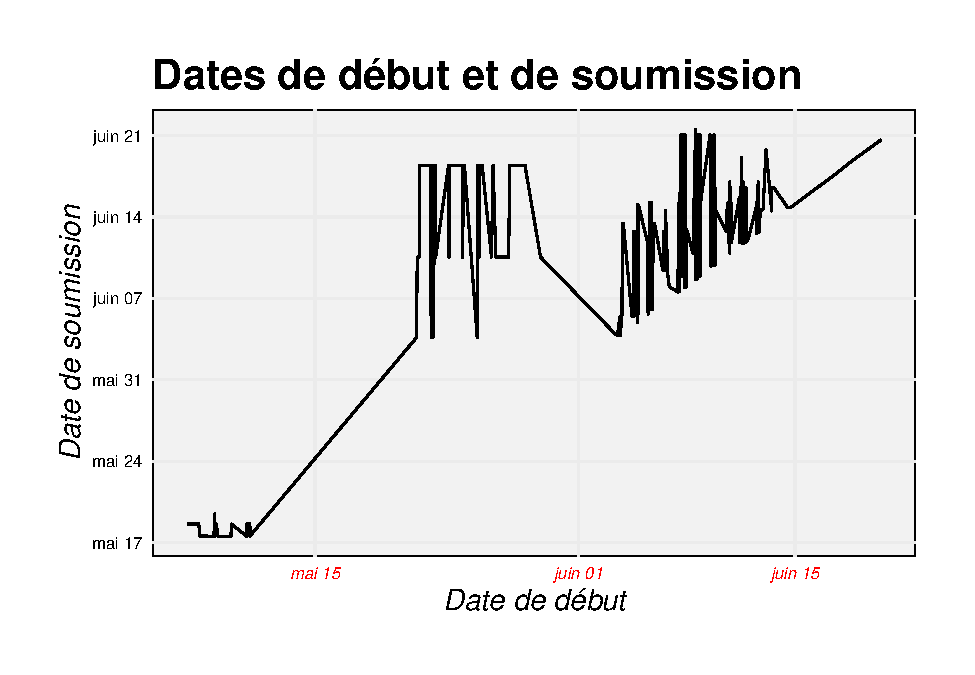
\includegraphics{PROJET_files/figure-latex/unnamed-chunk-14-1.pdf}

\begin{Shaded}
\begin{Highlighting}[]
\CommentTok{\#}
\end{Highlighting}
\end{Shaded}

\newpage

\begin{Shaded}
\begin{Highlighting}[]
\CommentTok{\#{-}{-}{-}{-}{-}{-}{-}{-}{-}{-}{-}{-}{-}{-}{-}{-}{-}{-}{-}{-}{-}{-}{-}{-}{-}{-}{-}{-}{-}{-}{-}{-}{-}{-}{-}{-}{-}{-}{-}{-}{-}{-}{-}{-}{-}{-}{-}{-}{-}{-}{-}{-}{-}{-}{-}{-}{-}{-}{-}{-}{-}{-}{-}{-}{-}{-}{-}{-}{-}{-}{-}{-}{-}{-}{-}{-}{-}{-}{-}{-}{-}{-}{-}{-}{-}{-}{-}{-}{-}}
\CommentTok{\#  Le graphique de densité avec geom\_density représentant }
\CommentTok{\#    la distribution des valeurs de la variable today }
\CommentTok{\#{-}{-}{-}{-}{-}{-}{-}{-}{-}{-}{-}{-}{-}{-}{-}{-}{-}{-}{-}{-}{-}{-}{-}{-}{-}{-}{-}{-}{-}{-}{-}{-}{-}{-}{-}{-}{-}{-}{-}{-}{-}{-}{-}{-}{-}{-}{-}{-}{-}{-}{-}{-}{-}{-}{-}{-}{-}{-}{-}{-}{-}{-}{-}{-}{-}{-}{-}{-}{-}{-}{-}{-}{-}{-}{-}{-}{-}{-}{-}{-}{-}{-}{-}{-}{-}{-}{-}{-}{-}}
\CommentTok{\# Un peu d\textquotesingle{}esthetique avec la fonction theme ()}
\CommentTok{\#{-}{-}{-}{-}{-}{-}{-}{-}{-}{-}{-}{-}{-}{-}{-}{-}{-}{-}{-}{-}{-}{-}{-}{-}{-}{-}{-}{-}{-}{-}{-}{-}{-}{-}{-}{-}{-}{-}{-}{-}{-}{-}{-}{-}{-}{-}{-}{-}{-}{-}{-}{-}{-}{-}{-}{-}{-}{-}{-}{-}{-}{-}{-}{-}{-}{-}{-}{-}{-}{-}{-}{-}{-}{-}{-}{-}{-}{-}{-}{-}{-}{-}{-}{-}{-}{-}{-}{-}{-}}

\FunctionTok{ggplot}\NormalTok{(projet) }\SpecialCharTok{+}
  
  \FunctionTok{aes}\NormalTok{(}\AttributeTok{x =}\NormalTok{ today) }\SpecialCharTok{+}
  
  \FunctionTok{geom\_density}\NormalTok{(}\AttributeTok{fill =} \StringTok{"\#e63946"}\NormalTok{, }\AttributeTok{col =} \StringTok{"black"}\NormalTok{, }\AttributeTok{show.legend =} \ConstantTok{FALSE}\NormalTok{) }\SpecialCharTok{+}
  
  \FunctionTok{ggtitle}\NormalTok{(}\StringTok{"Date de l’enquête"}\NormalTok{) }\SpecialCharTok{+}
  
  \FunctionTok{xlab}\NormalTok{(}\StringTok{"Heures"}\NormalTok{) }\SpecialCharTok{+}
  
  \FunctionTok{ylab}\NormalTok{(}\StringTok{"Densité"}\NormalTok{) }\SpecialCharTok{+}
  
  \FunctionTok{theme\_minimal}\NormalTok{() }\SpecialCharTok{+}
  
  \FunctionTok{theme}\NormalTok{(}
    
    \AttributeTok{plot.title =} \FunctionTok{element\_text}\NormalTok{(}\AttributeTok{color =} \StringTok{"black"}\NormalTok{, }\AttributeTok{size =} \DecValTok{20}\NormalTok{, }\AttributeTok{face =} \StringTok{"bold"}\NormalTok{),  }
    
    \AttributeTok{axis.text.x =} \FunctionTok{element\_text}\NormalTok{(}\AttributeTok{size =} \DecValTok{12}\NormalTok{),}
    
    \AttributeTok{axis.text.y =} \FunctionTok{element\_text}\NormalTok{(}\AttributeTok{size =} \DecValTok{12}\NormalTok{),}
    
    \AttributeTok{axis.title.x =} \FunctionTok{element\_text}\NormalTok{(}\AttributeTok{size =} \DecValTok{14}\NormalTok{),}
    
    \AttributeTok{axis.title.y =} \FunctionTok{element\_text}\NormalTok{(}\AttributeTok{size =} \DecValTok{14}\NormalTok{),}
    
    \AttributeTok{panel.grid.major =} \FunctionTok{element\_blank}\NormalTok{(),}
    
    \AttributeTok{panel.grid.minor =} \FunctionTok{element\_blank}\NormalTok{(),}
    
    \AttributeTok{panel.background =} \FunctionTok{element\_rect}\NormalTok{(}\AttributeTok{fill =} \StringTok{"\#F2F2F2"}\NormalTok{),}
    
    \AttributeTok{legend.position =} \StringTok{"bottom"}\NormalTok{,}
    
    \AttributeTok{legend.title =} \FunctionTok{element\_text}\NormalTok{(}\AttributeTok{size =} \DecValTok{12}\NormalTok{),}
    
    \AttributeTok{legend.text =} \FunctionTok{element\_text}\NormalTok{(}\AttributeTok{size =} \DecValTok{10}\NormalTok{),}
    
    \AttributeTok{legend.background =} \FunctionTok{element\_rect}\NormalTok{(}\AttributeTok{fill =} \StringTok{"white"}\NormalTok{, }\AttributeTok{color =} \StringTok{"black"}\NormalTok{),}
    
    \AttributeTok{plot.margin =} \FunctionTok{margin}\NormalTok{(}\DecValTok{1}\NormalTok{, }\DecValTok{1}\NormalTok{, }\DecValTok{1}\NormalTok{, }\DecValTok{1}\NormalTok{, }\StringTok{"cm"}\NormalTok{)}
\NormalTok{  )}
\end{Highlighting}
\end{Shaded}

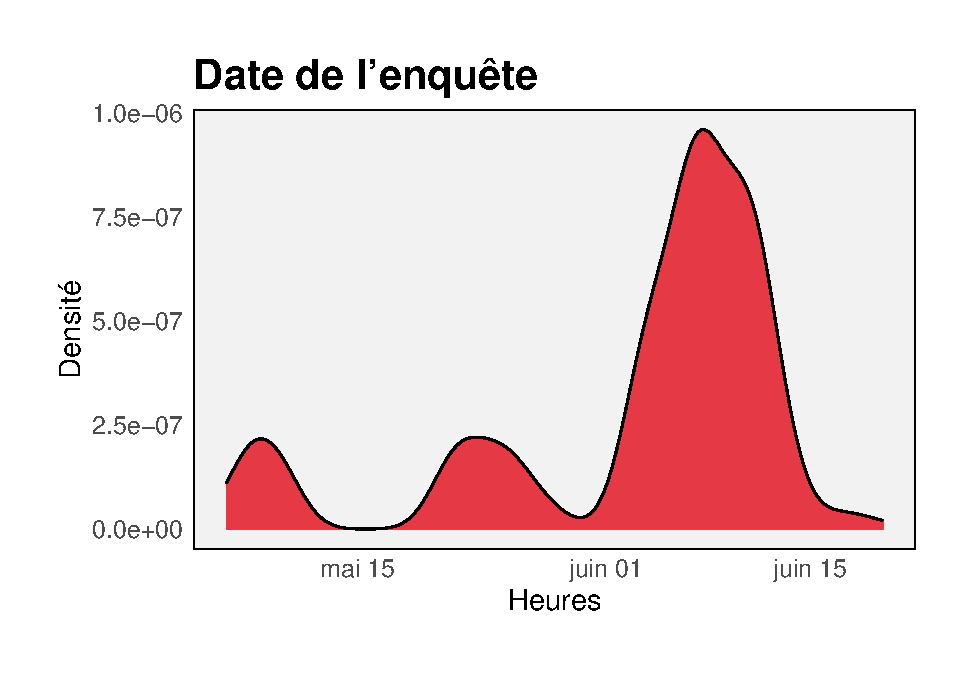
\includegraphics{PROJET_files/figure-latex/unnamed-chunk-15-1.pdf}

\begin{Shaded}
\begin{Highlighting}[]
\CommentTok{\#}
\end{Highlighting}
\end{Shaded}

\newpage

\begin{Shaded}
\begin{Highlighting}[]
\FunctionTok{library}\NormalTok{(GGally)}
\end{Highlighting}
\end{Shaded}

\begin{verbatim}
## Registered S3 method overwritten by 'GGally':
##   method from   
##   +.gg   ggplot2
\end{verbatim}

\begin{Shaded}
\begin{Highlighting}[]
\CommentTok{\#{-}{-}{-}{-}{-}{-}{-}{-}{-}{-}{-}{-}{-}{-}{-}{-}{-}{-}{-}{-}{-}{-}{-}{-}{-}{-}{-}{-}{-}{-}{-}{-}{-}{-}{-}{-}{-}{-}{-}{-}{-}{-}{-}{-}{-}{-}{-}{-}{-}{-}{-}{-}{-}{-}{-}{-}{-}{-}{-}{-}{-}{-}{-}{-}{-}{-}{-}{-}{-}{-}{-}{-}{-}{-}{-}{-}{-}{-}{-}{-}{-}{-}{-}{-}{-}{-}{-}{-}{-}{-}{-}}
\CommentTok{\# Creer une nouvelle variable Age }
\CommentTok{\#{-}{-}{-}{-}{-}{-}{-}{-}{-}{-}{-}{-}{-}{-}{-}{-}{-}{-}{-}{-}{-}{-}{-}{-}{-}{-}{-}{-}{-}{-}{-}{-}{-}{-}{-}{-}{-}{-}{-}{-}{-}{-}{-}{-}{-}{-}{-}{-}{-}{-}{-}{-}{-}{-}{-}{-}{-}{-}{-}{-}{-}{-}{-}{-}{-}{-}{-}{-}{-}{-}{-}{-}{-}{-}{-}{-}{-}{-}{-}{-}{-}{-}{-}{-}{-}{-}{-}{-}{-}{-}{-}}
\NormalTok{projet}\SpecialCharTok{$}\NormalTok{Age  }\OtherTok{=}\NormalTok{  projet}\SpecialCharTok{$}\NormalTok{q24 }

\CommentTok{\#{-}{-}{-}{-}{-}{-}{-}{-}{-}{-}{-}{-}{-}{-}{-}{-}{-}{-}{-}{-}{-}{-}{-}{-}{-}{-}{-}{-}{-}{-}{-}{-}{-}{-}{-}{-}{-}{-}{-}{-}{-}{-}{-}{-}{-}{-}{-}{-}{-}{-}{-}{-}{-}{-}{-}{-}{-}{-}{-}{-}{-}{-}{-}{-}{-}{-}{-}{-}{-}{-}{-}{-}{-}{-}{-}{-}{-}{-}{-}{-}{-}{-}{-}{-}{-}{-}{-}{-}{-}{-}}
\CommentTok{\# Filtrer les age inferieur a 120 pour etre realiste}
\CommentTok{\#{-}{-}{-}{-}{-}{-}{-}{-}{-}{-}{-}{-}{-}{-}{-}{-}{-}{-}{-}{-}{-}{-}{-}{-}{-}{-}{-}{-}{-}{-}{-}{-}{-}{-}{-}{-}{-}{-}{-}{-}{-}{-}{-}{-}{-}{-}{-}{-}{-}{-}{-}{-}{-}{-}{-}{-}{-}{-}{-}{-}{-}{-}{-}{-}{-}{-}{-}{-}{-}{-}{-}{-}{-}{-}{-}{-}{-}{-}{-}{-}{-}{-}{-}{-}{-}{-}{-}{-}{-}}

\NormalTok{Resume  }\OtherTok{=}\NormalTok{  projet }\SpecialCharTok{\%\textgreater{}\%}
  
  \FunctionTok{filter}\NormalTok{(   }
    
\NormalTok{    Age }\SpecialCharTok{\textless{}} \DecValTok{120} 
    
\NormalTok{    ) }\SpecialCharTok{\%\textgreater{}\%} 
  
  \FunctionTok{rename}\NormalTok{(}
    
    \AttributeTok{Proprietaire\_locataire =}\NormalTok{ q81,}\AttributeTok{Statut\_juridique  =}\NormalTok{ q12,}
    
    \AttributeTok{Niveau\_instruction =}\NormalTok{ q25}
    
\NormalTok{  )}

\CommentTok{\#{-}{-}{-}{-}{-}{-}{-}{-}{-}{-}{-}{-}{-}{-}{-}{-}{-}{-}{-}{-}{-}{-}{-}{-}{-}{-}{-}{-}{-}{-}{-}{-}{-}{-}{-}{-}{-}{-}{-}{-}{-}{-}{-}{-}{-}{-}{-}{-}{-}{-}{-}{-}{-}{-}{-}{-}{-}{-}{-}{-}{-}{-}{-}{-}{-}{-}{-}{-}{-}{-}{-}{-}{-}{-}{-}{-}{-}{-}{-}{-}{-}{-}{-}{-}{-}{-}{-}{-}{-}}
\CommentTok{\# Un exemple de resumer  des variable avec  ggbivariate()}
\CommentTok{\#{-}{-}{-}{-}{-}{-}{-}{-}{-}{-}{-}{-}{-}{-}{-}{-}{-}{-}{-}{-}{-}{-}{-}{-}{-}{-}{-}{-}{-}{-}{-}{-}{-}{-}{-}{-}{-}{-}{-}{-}{-}{-}{-}{-}{-}{-}{-}{-}{-}{-}{-}{-}{-}{-}{-}{-}{-}{-}{-}{-}{-}{-}{-}{-}{-}{-}{-}{-}{-}{-}{-}{-}{-}{-}{-}{-}{-}{-}{-}{-}{-}{-}{-}{-}{-}{-}{-}{-}{-}}

\FunctionTok{ggbivariate}\NormalTok{(}
  
  \AttributeTok{data =}\NormalTok{ Resume,}
            
            \AttributeTok{outcome =} \StringTok{"Proprietaire\_locataire"}\NormalTok{,}
            
            \AttributeTok{explanatory =} \FunctionTok{c}\NormalTok{(}\StringTok{"sexe"}\NormalTok{, }\StringTok{"Statut\_juridique"}\NormalTok{,}
                            
                            \StringTok{"Niveau\_instruction"}\NormalTok{, }\StringTok{"Age"}
\NormalTok{                            )}
\NormalTok{            )}
\end{Highlighting}
\end{Shaded}

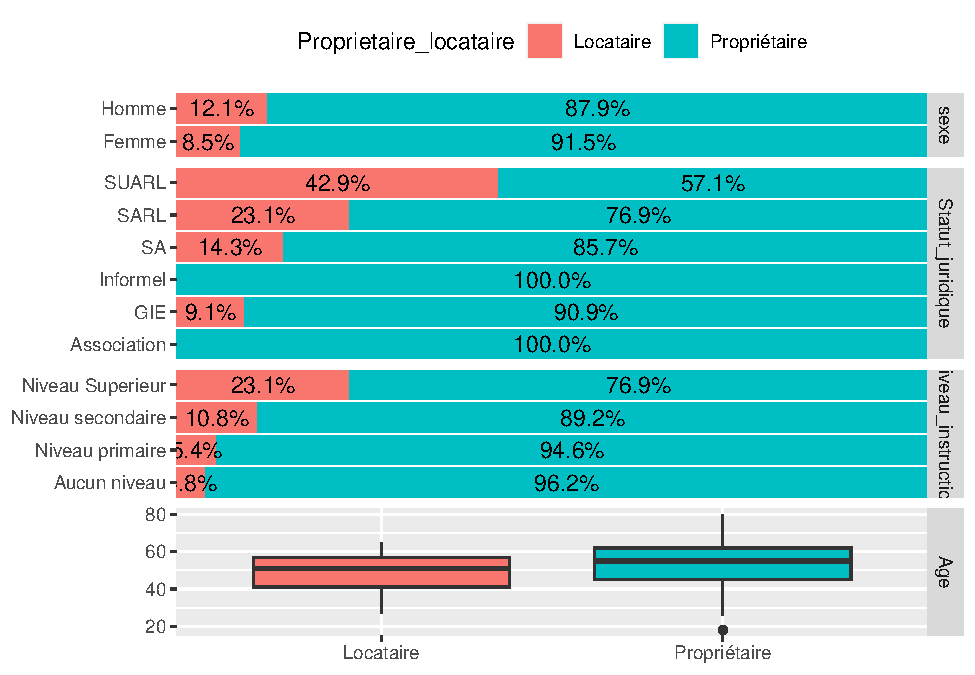
\includegraphics{PROJET_files/figure-latex/unnamed-chunk-16-1.pdf}

\begin{Shaded}
\begin{Highlighting}[]
\CommentTok{\#}
\end{Highlighting}
\end{Shaded}

\newpage

\begin{Shaded}
\begin{Highlighting}[]
\CommentTok{\#{-}{-}{-}{-}{-}{-}{-}{-}{-}{-}{-}{-}{-}{-}{-}{-}{-}{-}{-}{-}{-}{-}{-}{-}{-}{-}{-}{-}{-}{-}{-}{-}{-}{-}{-}{-}{-}{-}{-}{-}{-}{-}{-}{-}{-}{-}{-}{-}{-}{-}{-}{-}{-}{-}{-}{-}{-}{-}{-}{-}{-}{-}{-}{-}{-}{-}{-}{-}{-}{-}{-}{-}{-}{-}{-}{-}{-}{-}{-}{-}{-}{-}{-}{-}{-}{-}{-}}
\CommentTok{\#               Selection des langues et renommer }
\CommentTok{\#{-}{-}{-}{-}{-}{-}{-}{-}{-}{-}{-}{-}{-}{-}{-}{-}{-}{-}{-}{-}{-}{-}{-}{-}{-}{-}{-}{-}{-}{-}{-}{-}{-}{-}{-}{-}{-}{-}{-}{-}{-}{-}{-}{-}{-}{-}{-}{-}{-}{-}{-}{-}{-}{-}{-}{-}{-}{-}{-}{-}{-}{-}{-}{-}{-}{-}{-}{-}{-}{-}{-}{-}{-}{-}{-}{-}{-}{-}{-}{-}{-}{-}{-}{-}{-}{-}{-}{-}}
\NormalTok{vect\_langue }\OtherTok{=} \FunctionTok{c}\NormalTok{(}\StringTok{"francais"}\NormalTok{,}\StringTok{"wolof"}\NormalTok{,}
              \StringTok{"diola"}\NormalTok{,}\StringTok{"serere"}\NormalTok{,}\StringTok{"peul"}\NormalTok{,}
              \StringTok{"mandingue"}\NormalTok{,}\StringTok{"balante"}\NormalTok{,}\StringTok{"bambara"}\NormalTok{,}
              \StringTok{"autre\_langue"}\NormalTok{)}



\NormalTok{data }\OtherTok{\textless{}{-}}\NormalTok{ projet }\SpecialCharTok{\%\textgreater{}\%}
  
\NormalTok{  dplyr}\SpecialCharTok{::}\FunctionTok{select}\NormalTok{(}\FunctionTok{starts\_with}\NormalTok{(}\StringTok{"q24a\_"}\NormalTok{))}

\FunctionTok{names}\NormalTok{(data) }\OtherTok{=}\NormalTok{ vect\_langue}


\CommentTok{\#{-}{-}{-}{-}{-}{-}{-}{-}{-}{-}{-}{-}{-}{-}{-}{-}{-}{-}{-}{-}{-}{-}{-}{-}{-}{-}{-}{-}{-}{-}{-}{-}{-}{-}{-}{-}{-}{-}{-}{-}{-}{-}{-}{-}{-}{-}{-}{-}{-}{-}{-}{-}{-}{-}{-}{-}{-}{-}{-}{-}{-}{-}{-}{-}{-}{-}{-}{-}{-}{-}{-}{-}{-}{-}{-}{-}{-}{-}{-}{-}{-}{-}{-}{-}{-}{-}{-}{-}{-}{-}{-}}
\CommentTok{\#  Regrouper par langue en data1 ..... data9 }
\CommentTok{\#      i.e  Sommer le nombre de langue parler}
\CommentTok{\#{-}{-}{-}{-}{-}{-}{-}{-}{-}{-}{-}{-}{-}{-}{-}{-}{-}{-}{-}{-}{-}{-}{-}{-}{-}{-}{-}{-}{-}{-}{-}{-}{-}{-}{-}{-}{-}{-}{-}{-}{-}{-}{-}{-}{-}{-}{-}{-}{-}{-}{-}{-}{-}{-}{-}{-}{-}{-}{-}{-}{-}{-}{-}{-}{-}{-}{-}{-}{-}{-}{-}{-}{-}{-}{-}{-}{-}{-}{-}{-}{-}{-}{-}{-}{-}{-}{-}{-}{-}{-}{-}}

\NormalTok{data1 }\OtherTok{=}\NormalTok{  data }\SpecialCharTok{\%\textgreater{}\%}
\FunctionTok{filter}\NormalTok{(francais }\SpecialCharTok{==} \DecValTok{1}\NormalTok{) }\SpecialCharTok{\%\textgreater{}\%} 
\NormalTok{  dplyr}\SpecialCharTok{::}\FunctionTok{mutate}\NormalTok{(}\AttributeTok{francais =} \FunctionTok{ifelse}\NormalTok{(francais }\SpecialCharTok{==} \DecValTok{1}\NormalTok{, }\StringTok{"francais"}\NormalTok{))}\SpecialCharTok{\%\textgreater{}\%}
  \FunctionTok{group\_by}\NormalTok{(francais)}\SpecialCharTok{\%\textgreater{}\%}  
  \FunctionTok{count}\NormalTok{(}\AttributeTok{name =} \StringTok{"total\_langue"}\NormalTok{)}

\NormalTok{data2 }\OtherTok{=}\NormalTok{  data }\SpecialCharTok{\%\textgreater{}\%}
\FunctionTok{filter}\NormalTok{(wolof }\SpecialCharTok{==} \DecValTok{1}\NormalTok{) }\SpecialCharTok{\%\textgreater{}\%} 
\NormalTok{  dplyr}\SpecialCharTok{::}\FunctionTok{mutate}\NormalTok{(}\AttributeTok{wolof =} \FunctionTok{ifelse}\NormalTok{(wolof }\SpecialCharTok{==} \DecValTok{1}\NormalTok{, }\StringTok{"wolof"}\NormalTok{))}\SpecialCharTok{\%\textgreater{}\%}
  \FunctionTok{group\_by}\NormalTok{(wolof)}\SpecialCharTok{\%\textgreater{}\%} 
  \FunctionTok{count}\NormalTok{(}\AttributeTok{name =} \StringTok{"total\_langue"}\NormalTok{)}

\NormalTok{data3 }\OtherTok{=}\NormalTok{  data }\SpecialCharTok{\%\textgreater{}\%}
\FunctionTok{filter}\NormalTok{(diola }\SpecialCharTok{==} \DecValTok{1}\NormalTok{) }\SpecialCharTok{\%\textgreater{}\%} 
\NormalTok{  dplyr}\SpecialCharTok{::}\FunctionTok{mutate}\NormalTok{(}\AttributeTok{diola =} \FunctionTok{ifelse}\NormalTok{(diola }\SpecialCharTok{==} \DecValTok{1}\NormalTok{, }\StringTok{"diola"}\NormalTok{))}\SpecialCharTok{\%\textgreater{}\%} 
  \FunctionTok{group\_by}\NormalTok{(diola)}\SpecialCharTok{\%\textgreater{}\%} 
  \FunctionTok{count}\NormalTok{(}\AttributeTok{name =} \StringTok{"total\_langue"}\NormalTok{)}

\NormalTok{data4 }\OtherTok{=}\NormalTok{  data }\SpecialCharTok{\%\textgreater{}\%}
\FunctionTok{filter}\NormalTok{(serere }\SpecialCharTok{==} \DecValTok{1}\NormalTok{) }\SpecialCharTok{\%\textgreater{}\%}  
\NormalTok{  dplyr}\SpecialCharTok{::}\FunctionTok{mutate}\NormalTok{(}\AttributeTok{serere =} \FunctionTok{ifelse}\NormalTok{(serere }\SpecialCharTok{==} \DecValTok{1}\NormalTok{, }\StringTok{"serere"}\NormalTok{))}\SpecialCharTok{\%\textgreater{}\%}
  \FunctionTok{group\_by}\NormalTok{(serere)}\SpecialCharTok{\%\textgreater{}\%}  
  \FunctionTok{count}\NormalTok{(}\AttributeTok{name =} \StringTok{"total\_langue"}\NormalTok{)}

\NormalTok{data5 }\OtherTok{=}\NormalTok{  data }\SpecialCharTok{\%\textgreater{}\%}
\FunctionTok{filter}\NormalTok{(peul  }\SpecialCharTok{==} \DecValTok{1}\NormalTok{) }\SpecialCharTok{\%\textgreater{}\%}  
\NormalTok{  dplyr}\SpecialCharTok{::}\FunctionTok{mutate}\NormalTok{(}\AttributeTok{peul  =} \FunctionTok{ifelse}\NormalTok{(peul  }\SpecialCharTok{==} \DecValTok{1}\NormalTok{, }\StringTok{"peul"}\NormalTok{))}\SpecialCharTok{\%\textgreater{}\%} 
  \FunctionTok{group\_by}\NormalTok{(peul )}\SpecialCharTok{\%\textgreater{}\%} 
  \FunctionTok{count}\NormalTok{(}\AttributeTok{name =} \StringTok{"total\_langue"}\NormalTok{)}

\NormalTok{data6 }\OtherTok{=}\NormalTok{  data }\SpecialCharTok{\%\textgreater{}\%}
\FunctionTok{filter}\NormalTok{(mandingue  }\SpecialCharTok{==} \DecValTok{1}\NormalTok{) }\SpecialCharTok{\%\textgreater{}\%} 
\NormalTok{  dplyr}\SpecialCharTok{::}\FunctionTok{mutate}\NormalTok{(}\AttributeTok{mandingue  =} \FunctionTok{ifelse}\NormalTok{(mandingue  }\SpecialCharTok{==} \DecValTok{1}\NormalTok{, }\StringTok{"mandingue"}\NormalTok{))}\SpecialCharTok{\%\textgreater{}\%} 
  \FunctionTok{group\_by}\NormalTok{(mandingue)}\SpecialCharTok{\%\textgreater{}\%} 
  \FunctionTok{count}\NormalTok{(}\AttributeTok{name =} \StringTok{"total\_langue"}\NormalTok{)}


\NormalTok{data7 }\OtherTok{=}\NormalTok{  data }\SpecialCharTok{\%\textgreater{}\%}
\FunctionTok{filter}\NormalTok{(balante  }\SpecialCharTok{==} \DecValTok{1}\NormalTok{) }\SpecialCharTok{\%\textgreater{}\%} 
\NormalTok{  dplyr}\SpecialCharTok{::}\FunctionTok{mutate}\NormalTok{(}\AttributeTok{balante  =} \FunctionTok{ifelse}\NormalTok{(balante }\SpecialCharTok{==} \DecValTok{1}\NormalTok{, }\StringTok{"balante"}\NormalTok{))}\SpecialCharTok{\%\textgreater{}\%} 
  \FunctionTok{group\_by}\NormalTok{(balante)}\SpecialCharTok{\%\textgreater{}\%} 
  \FunctionTok{count}\NormalTok{(}\AttributeTok{name =} \StringTok{"total\_langue"}\NormalTok{)}

\NormalTok{data8 }\OtherTok{=}\NormalTok{  data }\SpecialCharTok{\%\textgreater{}\%}
\FunctionTok{filter}\NormalTok{(bambara  }\SpecialCharTok{==} \DecValTok{1}\NormalTok{) }\SpecialCharTok{\%\textgreater{}\%}
\NormalTok{  dplyr}\SpecialCharTok{::}\FunctionTok{mutate}\NormalTok{(}\AttributeTok{bambara  =} \FunctionTok{ifelse}\NormalTok{(bambara }\SpecialCharTok{==} \DecValTok{1}\NormalTok{, }\StringTok{"bambara"}\NormalTok{))}\SpecialCharTok{\%\textgreater{}\%} 
  \FunctionTok{group\_by}\NormalTok{(bambara)}\SpecialCharTok{\%\textgreater{}\%} 
  \FunctionTok{count}\NormalTok{(}\AttributeTok{name =} \StringTok{"total\_langue"}\NormalTok{)}

\NormalTok{data9 }\OtherTok{=}\NormalTok{  data }\SpecialCharTok{\%\textgreater{}\%}
\FunctionTok{filter}\NormalTok{(autre\_langue  }\SpecialCharTok{==} \DecValTok{1}\NormalTok{) }\SpecialCharTok{\%\textgreater{}\%} 
\NormalTok{  dplyr}\SpecialCharTok{::}\FunctionTok{mutate}\NormalTok{(}\AttributeTok{autre\_langue  =} \FunctionTok{ifelse}\NormalTok{(autre\_langue }\SpecialCharTok{==} \DecValTok{1}\NormalTok{, }\StringTok{"autre\_langue"}\NormalTok{))}\SpecialCharTok{\%\textgreater{}\%}
  \FunctionTok{group\_by}\NormalTok{(autre\_langue)}\SpecialCharTok{\%\textgreater{}\%} 
  \FunctionTok{count}\NormalTok{(}\AttributeTok{name =} \StringTok{"total\_langue"}\NormalTok{)}


\CommentTok{\#{-}{-}{-}{-}{-}{-}{-}{-}{-}{-}{-}{-}{-}{-}{-}{-}{-}{-}{-}{-}{-}{-}{-}{-}{-}{-}{-}{-}{-}{-}{-}{-}{-}{-}{-}{-}{-}{-}{-}{-}{-}{-}{-}{-}{-}{-}{-}{-}{-}{-}{-}{-}{-}{-}{-}{-}{-}{-}{-}{-}{-}{-}{-}{-}{-}{-}{-}{-}{-}{-}{-}{-}{-}{-}{-}{-}{-}{-}{-}{-}{-}{-}{-}{-}{-}{-}{-}{-}{-}{-}{-}{-}{-}{-}}
\CommentTok{\#    Fusionner les 10 data}
\CommentTok{\#{-}{-}{-}{-}{-}{-}{-}{-}{-}{-}{-}{-}{-}{-}{-}{-}{-}{-}{-}{-}{-}{-}{-}{-}{-}{-}{-}{-}{-}{-}{-}{-}{-}{-}{-}{-}{-}{-}{-}{-}{-}{-}{-}{-}{-}{-}{-}{-}{-}{-}{-}{-}{-}{-}{-}{-}{-}{-}{-}{-}{-}{-}{-}{-}{-}{-}{-}{-}{-}{-}{-}{-}{-}{-}{-}{-}{-}{-}{-}{-}{-}{-}{-}{-}{-}{-}{-}{-}{-}}

\NormalTok{LANGUE }\OtherTok{\textless{}{-}} \FunctionTok{bind\_rows}\NormalTok{(}
  
\NormalTok{data1 }\SpecialCharTok{\%\textgreater{}\%} 
  \FunctionTok{rename}\NormalTok{(}\AttributeTok{LANGUES =}\NormalTok{ francais),}

\NormalTok{data2 }\SpecialCharTok{\%\textgreater{}\%} 
  \FunctionTok{rename}\NormalTok{(}\AttributeTok{LANGUES =}\NormalTok{ wolof),}

\NormalTok{data3 }\SpecialCharTok{\%\textgreater{}\%} 
  \FunctionTok{rename}\NormalTok{(}\AttributeTok{LANGUES =}\NormalTok{ diola),}

\NormalTok{data4 }\SpecialCharTok{\%\textgreater{}\%} 
  \FunctionTok{rename}\NormalTok{(}\AttributeTok{LANGUES =}\NormalTok{ serere),}

\NormalTok{data5 }\SpecialCharTok{\%\textgreater{}\%} 
  \FunctionTok{rename}\NormalTok{(}\AttributeTok{LANGUES =}\NormalTok{ peul),}

\NormalTok{data6 }\SpecialCharTok{\%\textgreater{}\%} 
  \FunctionTok{rename}\NormalTok{(}\AttributeTok{LANGUES =}\NormalTok{ mandingue),}

\NormalTok{data7 }\SpecialCharTok{\%\textgreater{}\%} 
  \FunctionTok{rename}\NormalTok{(}\AttributeTok{LANGUES =}\NormalTok{ balante),}

\NormalTok{data8 }\SpecialCharTok{\%\textgreater{}\%} 
  \FunctionTok{rename}\NormalTok{(}\AttributeTok{LANGUES =}\NormalTok{ bambara),}

\NormalTok{data9 }\SpecialCharTok{\%\textgreater{}\%} 
  \FunctionTok{rename}\NormalTok{(}\AttributeTok{LANGUES =}\NormalTok{ autre\_langue)}
\NormalTok{)}


\CommentTok{\#{-}{-}{-}{-}{-}{-}{-}{-}{-}{-}{-}{-}{-}{-}{-}{-}{-}{-}{-}{-}{-}{-}{-}{-}{-}{-}{-}{-}{-}{-}{-}{-}{-}{-}{-}{-}{-}{-}{-}{-}{-}{-}{-}{-}{-}{-}{-}{-}{-}{-}{-}{-}{-}{-}{-}{-}{-}{-}{-}{-}{-}{-}{-}{-}{-}{-}{-}{-}{-}{-}{-}{-}{-}{-}{-}{-}{-}{-}{-}{-}{-}{-}{-}{-}{-}{-}{-}{-}{-}{-}}
\CommentTok{\#  Créer un graphique à barres à partir du dataframe avec geom\_bar}
\CommentTok{\#{-}{-}{-}{-}{-}{-}{-}{-}{-}{-}{-}{-}{-}{-}{-}{-}{-}{-}{-}{-}{-}{-}{-}{-}{-}{-}{-}{-}{-}{-}{-}{-}{-}{-}{-}{-}{-}{-}{-}{-}{-}{-}{-}{-}{-}{-}{-}{-}{-}{-}{-}{-}{-}{-}{-}{-}{-}{-}{-}{-}{-}{-}{-}{-}{-}{-}{-}{-}{-}{-}{-}{-}{-}{-}{-}{-}{-}{-}{-}{-}{-}{-}{-}{-}{-}{-}{-}{-}{-}{-}}

\FunctionTok{ggplot}\NormalTok{( }\AttributeTok{data =}\NormalTok{ LANGUE , }\FunctionTok{aes}\NormalTok{( }\AttributeTok{x=}\NormalTok{ LANGUES, }\AttributeTok{y =}\NormalTok{ total\_langue, }\AttributeTok{fill =}\NormalTok{ LANGUES ))}\SpecialCharTok{+}
  
\FunctionTok{geom\_bar}\NormalTok{( }\AttributeTok{stat =} \StringTok{"identity"}\NormalTok{)}\SpecialCharTok{+}
  
  \FunctionTok{labs}\NormalTok{(}\AttributeTok{title =} \StringTok{"GRAPHIQUE DES LANGUES PARLEES"}\NormalTok{,}
       \AttributeTok{x =} \StringTok{"Langue"}\NormalTok{  ,}
       \AttributeTok{y =}\StringTok{""}\NormalTok{)}\SpecialCharTok{+}
  
\FunctionTok{theme\_minimal}\NormalTok{()}\SpecialCharTok{+}
  
\FunctionTok{coord\_polar}\NormalTok{(}\AttributeTok{start =} \DecValTok{0}\NormalTok{)}\SpecialCharTok{+}
  
\FunctionTok{ylim}\NormalTok{( }\SpecialCharTok{{-}}\DecValTok{50}\NormalTok{, }\DecValTok{300}\NormalTok{)}\SpecialCharTok{+}
  \FunctionTok{theme}\NormalTok{(}
    \AttributeTok{plot.title =} \FunctionTok{element\_text}\NormalTok{(}\AttributeTok{color =} \StringTok{"black"}\NormalTok{, }\AttributeTok{size =} \DecValTok{20}\NormalTok{, }\AttributeTok{face =} \StringTok{"bold"}\NormalTok{)}
\NormalTok{  )}
\end{Highlighting}
\end{Shaded}

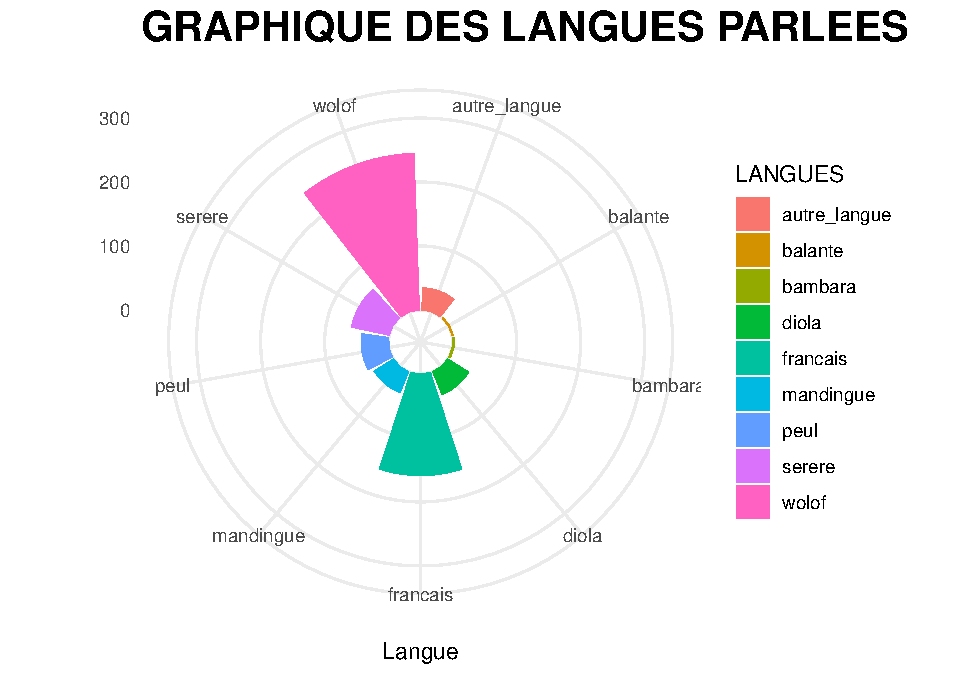
\includegraphics{PROJET_files/figure-latex/unnamed-chunk-17-1.pdf}

\begin{Shaded}
\begin{Highlighting}[]
\CommentTok{\#}
\end{Highlighting}
\end{Shaded}

\newpage

\begin{Shaded}
\begin{Highlighting}[]
\CommentTok{\#{-}{-}{-}{-}{-}{-}{-}{-}{-}{-}{-}{-}{-}{-}{-}{-}{-}{-}{-}{-}{-}{-}{-}{-}{-}{-}{-}{-}{-}{-}{-}{-}{-}{-}{-}{-}{-}{-}{-}{-}{-}{-}{-}{-}{-}{-}{-}{-}{-}{-}{-}{-}{-}{-}{-}{-}{-}{-}{-}{-}{-}{-}{-}{-}{-}{-}{-}{-}{-}{-}{-}{-}{-}{-}{-}{-}{-}{-}{-}{-}{-}{-}{-}{-}{-}{-}{-}{-}{-}{-}}
\CommentTok{\#  Créer un graphique à barres à partir du dataframe avec geom\_bar}
\CommentTok{\#{-}{-}{-}{-}{-}{-}{-}{-}{-}{-}{-}{-}{-}{-}{-}{-}{-}{-}{-}{-}{-}{-}{-}{-}{-}{-}{-}{-}{-}{-}{-}{-}{-}{-}{-}{-}{-}{-}{-}{-}{-}{-}{-}{-}{-}{-}{-}{-}{-}{-}{-}{-}{-}{-}{-}{-}{-}{-}{-}{-}{-}{-}{-}{-}{-}{-}{-}{-}{-}{-}{-}{-}{-}{-}{-}{-}{-}{-}{-}{-}{-}{-}{-}{-}{-}{-}{-}{-}{-}{-}}


\NormalTok{Instruction }\OtherTok{=}\NormalTok{ projet }\SpecialCharTok{\%\textgreater{}\%}
  
  \FunctionTok{rename}\NormalTok{(}\AttributeTok{Niveau\_instruction =}\NormalTok{ q25)}


\FunctionTok{ggplot}\NormalTok{(}\AttributeTok{data =}\NormalTok{ Instruction )}\SpecialCharTok{+}
  
  \FunctionTok{geom\_bar}\NormalTok{(}\FunctionTok{aes}\NormalTok{( }\AttributeTok{x =}\NormalTok{Niveau\_instruction,}
                \AttributeTok{y =}\NormalTok{ ..prop..,}\AttributeTok{group =} \DecValTok{1}\NormalTok{ , }
                \AttributeTok{fill =}\NormalTok{ ..count..), }
           \AttributeTok{col =} \StringTok{"green"}\NormalTok{, }\AttributeTok{width =} \FloatTok{0.7}\NormalTok{)}\SpecialCharTok{+}
  
  \FunctionTok{labs}\NormalTok{(}\AttributeTok{x=} \StringTok{"Niveau d\textquotesingle{}instruction"}\NormalTok{, }\AttributeTok{y =} \StringTok{"Nombre d\textquotesingle{}observation"}\NormalTok{)}\SpecialCharTok{+}
  
  \FunctionTok{theme\_minimal}\NormalTok{() }\SpecialCharTok{+}  
  
  \FunctionTok{theme}\NormalTok{(}
    \AttributeTok{panel.grid =} \FunctionTok{element\_blank}\NormalTok{(),}
    
    \AttributeTok{panel.border =} \FunctionTok{element\_blank}\NormalTok{(),}
    
    \AttributeTok{axis.text.y =} \FunctionTok{element\_blank}\NormalTok{(),}
    
    \AttributeTok{axis.ticks =} \FunctionTok{element\_blank}\NormalTok{(),}
    
    \AttributeTok{legend.position =} \StringTok{"top"}
\NormalTok{  )}
\end{Highlighting}
\end{Shaded}

\begin{verbatim}
## Warning: The dot-dot notation (`..prop..`) was deprecated in ggplot2 3.4.0.
## i Please use `after_stat(prop)` instead.
## This warning is displayed once every 8 hours.
## Call `lifecycle::last_lifecycle_warnings()` to see where this warning was
## generated.
\end{verbatim}

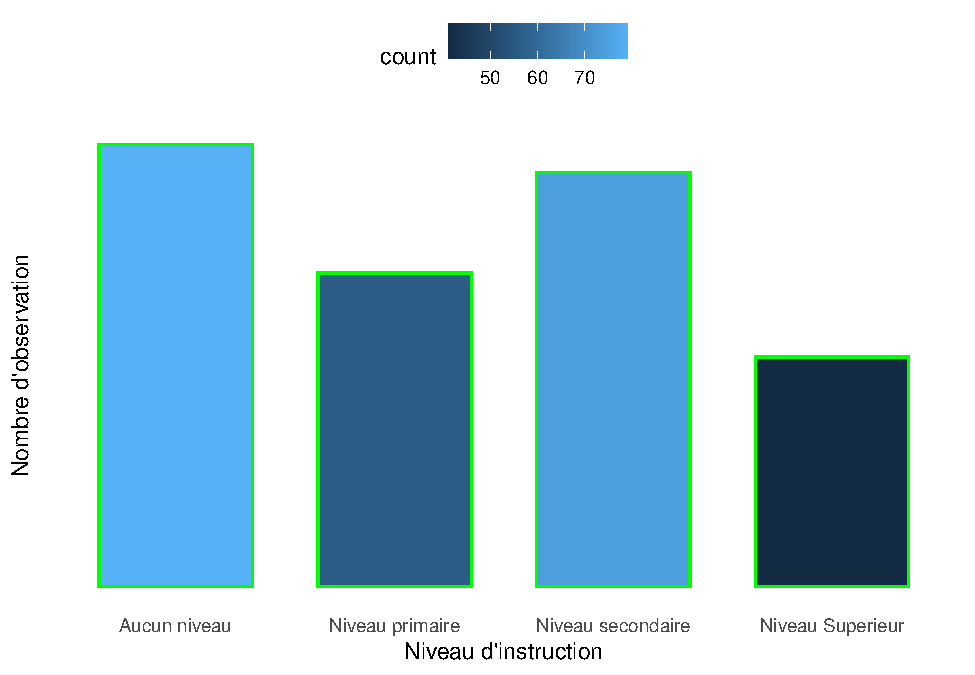
\includegraphics{PROJET_files/figure-latex/unnamed-chunk-18-1.pdf}

\begin{Shaded}
\begin{Highlighting}[]
\CommentTok{\#{-}{-}{-}{-}{-}{-}{-}{-}{-}{-}{-}{-}{-}{-}{-}{-}{-}{-}{-}{-}{-}{-}{-}{-}{-}{-}{-}{-}{-}{-}{-}{-}{-}{-}{-}{-}{-}{-}{-}{-}{-}{-}{-}{-}{-}{-}{-}{-}{-}{-}{-}{-}{-}{-}{-}{-}{-}{-}{-}{-}{-}{-}{-}{-}{-}{-}{-}{-}{-}{-}{-}{-}{-}{-}{-}{-}{-}{-}{-}{-}{-}{-}{-}{-}{-}{-}}
\end{Highlighting}
\end{Shaded}

\begin{Shaded}
\begin{Highlighting}[]
\NormalTok{Instruction }\OtherTok{=}\NormalTok{ projet }\SpecialCharTok{\%\textgreater{}\%}
  
  \FunctionTok{rename}\NormalTok{(}\AttributeTok{Niveau\_instruction =}\NormalTok{ q25)}


\CommentTok{\#{-}{-}{-}{-}{-}{-}{-}{-}{-}{-}{-}{-}{-}{-}{-}{-}{-}{-}{-}{-}{-}{-}{-}{-}{-}{-}{-}{-}{-}{-}{-}{-}{-}{-}{-}{-}{-}{-}{-}{-}{-}{-}{-}{-}{-}{-}{-}{-}{-}{-}{-}{-}{-}{-}{-}{-}{-}{-}{-}{-}{-}{-}{-}{-}{-}{-}{-}{-}{-}{-}{-}{-}{-}{-}{-}{-}{-}{-}{-}{-}{-}{-}{-}{-}{-}{-}}

\NormalTok{Instruction}\SpecialCharTok{$}\NormalTok{Age }\OtherTok{\textless{}{-}}\NormalTok{ Instruction}\SpecialCharTok{$}\NormalTok{q24 }\SpecialCharTok{\textgreater{}} \FunctionTok{median}\NormalTok{(Instruction}\SpecialCharTok{$}\NormalTok{q24)}

\CommentTok{\#{-}{-}{-}{-}{-}{-}{-}{-}{-}{-}{-}{-}{-}{-}{-}{-}{-}{-}{-}{-}{-}{-}{-}{-}{-}{-}{-}{-}{-}{-}{-}{-}{-}{-}{-}{-}{-}{-}{-}{-}{-}{-}{-}{-}{-}{-}{-}{-}{-}{-}{-}{-}{-}{-}{-}{-}{-}{-}{-}{-}{-}{-}{-}{-}{-}{-}{-}{-}{-}{-}{-}{-}{-}{-}{-}{-}{-}{-}{-}{-}{-}{-}{-}{-}{-}{-}}

\CommentTok{\#{-}{-}{-}{-}{-}{-}{-}{-}{-}{-}{-}{-}{-}{-}{-}{-}{-}{-}{-}{-}{-}{-}{-}{-}{-}{-}{-}{-}{-}{-}{-}{-}{-}{-}{-}{-}{-}{-}{-}{-}{-}{-}{-}{-}{-}{-}{-}{-}{-}{-}{-}{-}{-}{-}{-}{-}{-}{-}{-}{-}{-}{-}{-}{-}{-}{-}{-}{-}{-}{-}{-}{-}{-}{-}{-}{-}{-}{-}{-}{-}{-}{-}{-}{-}{-}{-}{-}{-}{-}{-}}
\CommentTok{\#  Créer un graphique à barres à partir du dataframe avec geom\_bar}
\CommentTok{\#{-}{-}{-}{-}{-}{-}{-}{-}{-}{-}{-}{-}{-}{-}{-}{-}{-}{-}{-}{-}{-}{-}{-}{-}{-}{-}{-}{-}{-}{-}{-}{-}{-}{-}{-}{-}{-}{-}{-}{-}{-}{-}{-}{-}{-}{-}{-}{-}{-}{-}{-}{-}{-}{-}{-}{-}{-}{-}{-}{-}{-}{-}{-}{-}{-}{-}{-}{-}{-}{-}{-}{-}{-}{-}{-}{-}{-}{-}{-}{-}{-}{-}{-}{-}{-}{-}{-}{-}{-}{-}}

\FunctionTok{ggplot}\NormalTok{(}\AttributeTok{data =}\NormalTok{ Instruction) }\SpecialCharTok{+} 
  
  \FunctionTok{geom\_bar}\NormalTok{(}\FunctionTok{aes}\NormalTok{(}\AttributeTok{x =}\NormalTok{ Niveau\_instruction, }\AttributeTok{fill =}\NormalTok{ Age),}
           
           \AttributeTok{position =} \StringTok{"dodge"}\NormalTok{, }\AttributeTok{width =} \FloatTok{0.4}\NormalTok{) }\SpecialCharTok{+}
  
  \FunctionTok{theme\_minimal}\NormalTok{() }\SpecialCharTok{+} 
  
  \FunctionTok{theme}\NormalTok{(}
    \AttributeTok{panel.grid =} \FunctionTok{element\_blank}\NormalTok{(),}
    
    \AttributeTok{panel.border =} \FunctionTok{element\_blank}\NormalTok{(),}
    
    \AttributeTok{axis.text.y =} \FunctionTok{element\_blank}\NormalTok{(),}
    
    \AttributeTok{axis.ticks =} \FunctionTok{element\_blank}\NormalTok{(),}
    
    \AttributeTok{legend.position =} \StringTok{"top"}
\NormalTok{  )}
\end{Highlighting}
\end{Shaded}

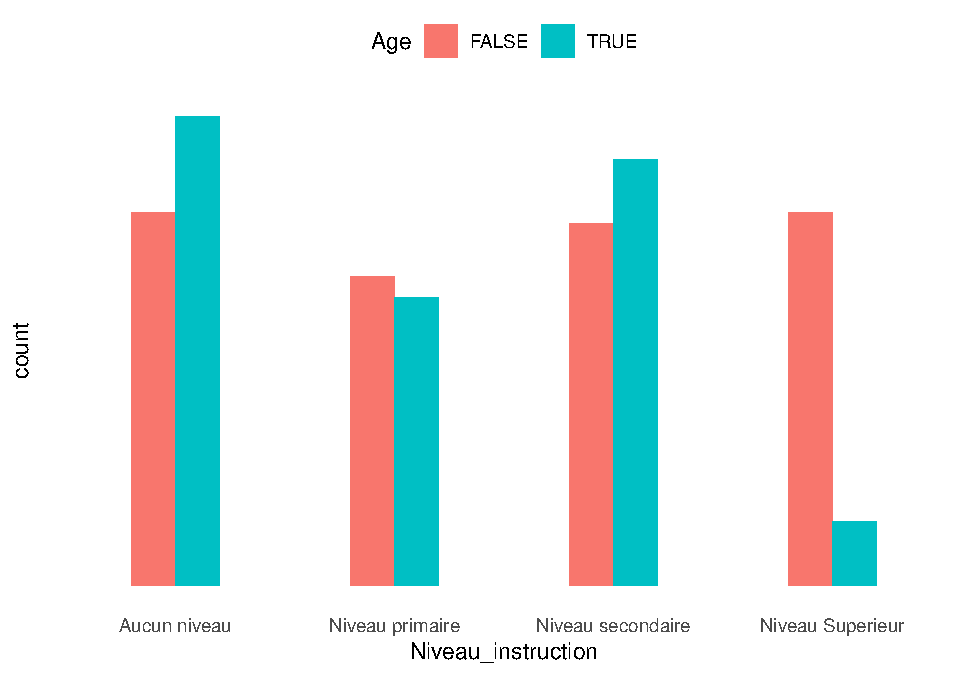
\includegraphics{PROJET_files/figure-latex/unnamed-chunk-19-1.pdf}

\begin{Shaded}
\begin{Highlighting}[]
\CommentTok{\#{-}{-}{-}{-}{-}{-}{-}{-}{-}{-}{-}{-}{-}{-}{-}{-}{-}{-}{-}{-}{-}{-}{-}{-}{-}{-}{-}{-}{-}{-}{-}{-}{-}{-}{-}{-}{-}{-}{-}{-}{-}{-}{-}{-}{-}{-}{-}{-}{-}{-}{-}{-}{-}{-}{-}{-}{-}{-}{-}{-}{-}{-}{-}{-}{-}{-}{-}{-}{-}{-}{-}{-}{-}{-}{-}{-}{-}{-}{-}{-}{-}{-}{-}{-}{-}{-}{-}{-}{-}{-}{-}{-}{-}{-}{-}{-}}
\CommentTok{\#     En fonction du niveau d\textquotesingle{}instruction, nous affichons ceux qui ont un age superieur a la mediane }
\CommentTok{\#      et ceux inferieur a la medianne . Alors on a vrai}
\CommentTok{\#           pour ceux superieur a la moyenne et faux sinon}
\CommentTok{\#{-}{-}{-}{-}{-}{-}{-}{-}{-}{-}{-}{-}{-}{-}{-}{-}{-}{-}{-}{-}{-}{-}{-}{-}{-}{-}{-}{-}{-}{-}{-}{-}{-}{-}{-}{-}{-}{-}{-}{-}{-}{-}{-}{-}{-}{-}{-}{-}{-}{-}{-}{-}{-}{-}{-}{-}{-}{-}{-}{-}{-}{-}{-}{-}{-}{-}{-}{-}{-}{-}{-}{-}{-}{-}{-}{-}{-}{-}{-}{-}{-}{-}{-}{-}{-}{-}{-}{-}}
\end{Highlighting}
\end{Shaded}

\begin{Shaded}
\begin{Highlighting}[]
\CommentTok{\#{-}{-}{-}{-}{-}{-}{-}{-}{-}{-}{-}{-}{-}{-}{-}{-}{-}{-}{-}{-}{-}{-}{-}{-}{-}{-}{-}{-}{-}{-}{-}{-}{-}{-}{-}{-}{-}{-}{-}{-}{-}{-}{-}{-}{-}{-}{-}{-}{-}{-}{-}{-}{-}{-}{-}{-}{-}{-}{-}{-}{-}}

\NormalTok{Statut }\OtherTok{\textless{}{-}}\NormalTok{ projet }\SpecialCharTok{\%\textgreater{}\%}
  
  \FunctionTok{rename}\NormalTok{(}\AttributeTok{Statut\_juridique =}\NormalTok{ q12,}
                           
                           \AttributeTok{Proprietaire\_locataire =}\NormalTok{ q81)}

\CommentTok{\# {-}{-}{-}{-}{-}{-}{-}{-}{-}{-}{-}{-}{-}{-}{-}{-}{-}{-}{-}{-}{-}{-}{-}{-}{-}{-}{-}{-}{-}{-}{-}{-}{-}{-}{-}{-}{-}{-}{-}{-}{-}{-}{-}{-}{-}{-}{-}{-}{-}{-}{-}{-}{-}{-}{-}{-}{-}{-}{-}{-}{-}{-}{-}{-}{-}{-}{-}{-}{-}{-}{-}{-}{-}{-}{-}{-}{-}{-}{-}{-}{-}{-}{-}{-}{-}{-}{-}{-}{-}}
\CommentTok{\#   Calculer la proportion des différents statuts juridiques}
\CommentTok{\#     pour chaque catégorie de propriétaire/locataire}
\CommentTok{\#{-}{-}{-}{-}{-}{-}{-}{-}{-}{-}{-}{-}{-}{-}{-}{-}{-}{-}{-}{-}{-}{-}{-}{-}{-}{-}{-}{-}{-}{-}{-}{-}{-}{-}{-}{-}{-}{-}{-}{-}{-}{-}{-}{-}{-}{-}{-}{-}{-}{-}{-}{-}{-}{-}{-}{-}{-}{-}{-}{-}{-}{-}{-}{-}{-}{-}{-}{-}{-}{-}{-}{-}{-}{-}{-}{-}{-}{-}{-}{-}{-}{-}{-}{-}{-}{-}{-}{-}{-}{-}}

\NormalTok{prop\_data }\OtherTok{\textless{}{-}}\NormalTok{ Statut }\SpecialCharTok{\%\textgreater{}\%}
  
  \FunctionTok{group\_by}\NormalTok{(Proprietaire\_locataire, Statut\_juridique) }\SpecialCharTok{\%\textgreater{}\%}
  
  \FunctionTok{summarize}\NormalTok{(}\AttributeTok{Proportion =} \FunctionTok{n}\NormalTok{()) }\SpecialCharTok{\%\textgreater{}\%}
  
  \FunctionTok{group\_by}\NormalTok{(Proprietaire\_locataire) }\SpecialCharTok{\%\textgreater{}\%}
  
  \FunctionTok{mutate}\NormalTok{(}\AttributeTok{Proportion =}\NormalTok{ Proportion }\SpecialCharTok{/} \FunctionTok{sum}\NormalTok{(Proportion))}
\end{Highlighting}
\end{Shaded}

\begin{verbatim}
## `summarise()` has grouped output by 'Proprietaire_locataire'. You can override
## using the `.groups` argument.
\end{verbatim}

\begin{Shaded}
\begin{Highlighting}[]
\CommentTok{\#{-}{-}{-}{-}{-}{-}{-}{-}{-}{-}{-}{-}{-}{-}{-}{-}{-}{-}{-}{-}{-}{-}{-}{-}{-}{-}{-}{-}{-}{-}{-}{-}{-}{-}{-}{-}{-}{-}{-}{-}{-}{-}{-}{-}{-}{-}{-}{-}{-}{-}{-}{-}{-}{-}{-}{-}{-}{-}{-}{-}{-}{-}{-}{-}{-}{-}{-}{-}{-}{-}{-}{-}{-}{-}{-}{-}{-}{-}{-}{-}{-}{-}{-}{-}{-}{-}{-}{-}{-}}
\CommentTok{\# Création du graphique à barres empilées}
\CommentTok{\#{-}{-}{-}{-}{-}{-}{-}{-}{-}{-}{-}{-}{-}{-}{-}{-}{-}{-}{-}{-}{-}{-}{-}{-}{-}{-}{-}{-}{-}{-}{-}{-}{-}{-}{-}{-}{-}{-}{-}{-}{-}{-}{-}{-}{-}{-}{-}{-}{-}{-}{-}{-}{-}{-}{-}{-}{-}{-}{-}{-}{-}{-}{-}{-}{-}{-}{-}{-}{-}{-}{-}{-}{-}{-}{-}{-}{-}{-}{-}{-}{-}{-}{-}{-}{-}{-}{-}{-}}

\FunctionTok{ggplot}\NormalTok{(}\AttributeTok{data =}\NormalTok{ prop\_data, }\FunctionTok{aes}\NormalTok{(}\AttributeTok{x =}\NormalTok{ Proprietaire\_locataire, }\AttributeTok{y =}\NormalTok{ Proportion, }\AttributeTok{fill =}\NormalTok{ Statut\_juridique)) }\SpecialCharTok{+}
  
  \FunctionTok{geom\_bar}\NormalTok{(}\AttributeTok{stat =} \StringTok{"identity"}\NormalTok{, }\AttributeTok{width =} \FloatTok{0.6}\NormalTok{) }\SpecialCharTok{+}
  
  \FunctionTok{xlab}\NormalTok{(}\StringTok{"Statut juridique"}\NormalTok{) }\SpecialCharTok{+}
  
  \FunctionTok{ylab}\NormalTok{(}\StringTok{"Proportion"}\NormalTok{) }\SpecialCharTok{+}
  
  \FunctionTok{labs}\NormalTok{(}\AttributeTok{fill =} \StringTok{"Statut juridique"}\NormalTok{) }\SpecialCharTok{+}
  
  \FunctionTok{scale\_y\_continuous}\NormalTok{(}\AttributeTok{labels =}\NormalTok{ scales}\SpecialCharTok{::}\NormalTok{percent) }\SpecialCharTok{+}
  
  \FunctionTok{scale\_fill\_brewer}\NormalTok{(}\AttributeTok{palette =} \StringTok{"Set1"}\NormalTok{) }\SpecialCharTok{+}

  \FunctionTok{theme\_minimal}\NormalTok{() }\SpecialCharTok{+}
  
  \FunctionTok{theme}\NormalTok{(}
    \AttributeTok{panel.background =} \FunctionTok{element\_rect}\NormalTok{(}\AttributeTok{fill =} \StringTok{"\#F0F0F0"}\NormalTok{),}
    \AttributeTok{axis.text.x =} \FunctionTok{element\_text}\NormalTok{(}\AttributeTok{angle =} \DecValTok{45}\NormalTok{, }\AttributeTok{hjust =} \DecValTok{1}\NormalTok{),}
    \AttributeTok{legend.position =} \StringTok{"top"}
\NormalTok{  )}
\end{Highlighting}
\end{Shaded}

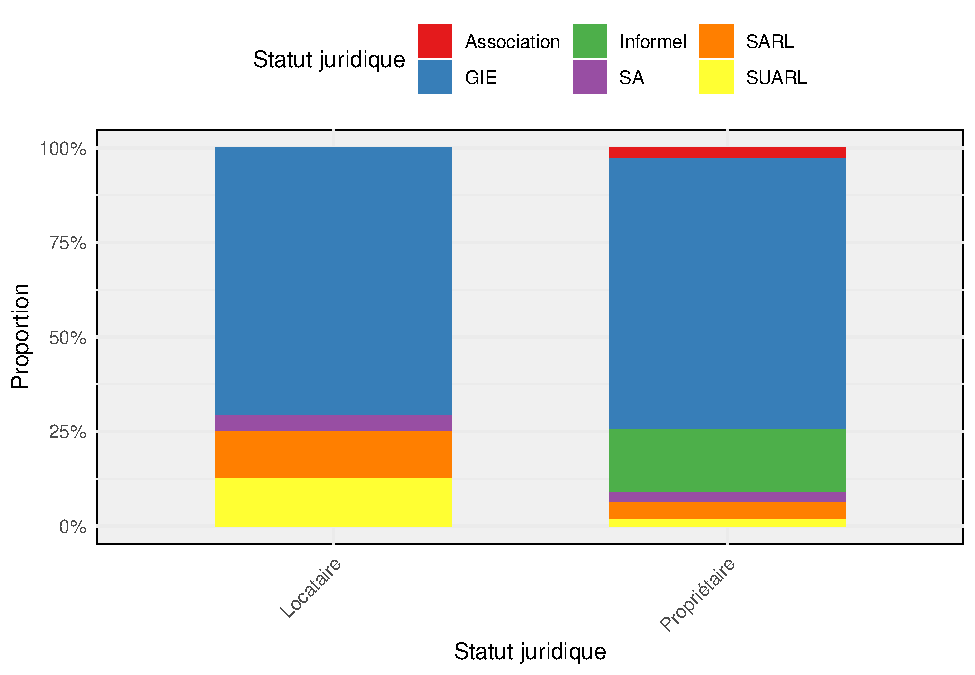
\includegraphics{PROJET_files/figure-latex/unnamed-chunk-20-1.pdf}

\begin{Shaded}
\begin{Highlighting}[]
\CommentTok{\#}
\end{Highlighting}
\end{Shaded}

\begin{Shaded}
\begin{Highlighting}[]
\CommentTok{\#{-}{-}{-}{-}{-}{-}{-}{-}{-}{-}{-}{-}{-}{-}{-}{-}{-}{-}{-}{-}{-}{-}{-}{-}{-}{-}{-}{-}{-}{-}{-}{-}{-}{-}{-}{-}{-}{-}{-}{-}{-}{-}{-}{-}{-}{-}{-}{-}{-}{-}{-}{-}{-}{-}{-}{-}{-}{-}{-}{-}{-}{-}{-}{-}{-}{-}{-}{-}{-}{-}{-}{-}{-}{-}{-}{-}{-}{-}{-}{-}{-}{-}{-}{-}{-}{-}{-}}
\CommentTok{\# Une boite a moustache avec les individus agés de moins 120 ans  pour rester dans une realité}
\CommentTok{\# Du fait qu\textquotesingle{}il existe des valeurs exorbitante dans la variable age }
\CommentTok{\#{-}{-}{-}{-}{-}{-}{-}{-}{-}{-}{-}{-}{-}{-}{-}{-}{-}{-}{-}{-}{-}{-}{-}{-}{-}{-}{-}{-}{-}{-}{-}{-}{-}{-}{-}{-}{-}{-}{-}{-}{-}{-}{-}{-}{-}{-}{-}{-}{-}{-}{-}{-}{-}{-}{-}{-}{-}{-}{-}{-}{-}{-}{-}{-}{-}{-}{-}{-}{-}{-}{-}{-}{-}{-}{-}{-}{-}{-}{-}{-}{-}{-}{-}{-}{-}{-}{-}}

\NormalTok{projet}\SpecialCharTok{$}\NormalTok{Age }\OtherTok{\textless{}{-}}\NormalTok{ projet}\SpecialCharTok{$}\NormalTok{q24}

\NormalTok{Boite\_moustache }\OtherTok{=}\NormalTok{  projet }\SpecialCharTok{\%\textgreater{}\%}
\FunctionTok{filter}\NormalTok{( Age }\SpecialCharTok{\textless{}} \DecValTok{120}\NormalTok{ )}

\FunctionTok{boxplot}\NormalTok{(Boite\_moustache}\SpecialCharTok{$}\NormalTok{Age,}
        
\AttributeTok{ylab =} \StringTok{"Age"}\NormalTok{,}

\AttributeTok{main =} \StringTok{"Boite à moustache des proprietaires en age"}\NormalTok{,}

\AttributeTok{col =} \StringTok{"\#e63946"}\NormalTok{,}

\AttributeTok{las =} \DecValTok{1}\NormalTok{ ,}

\AttributeTok{cex.main =} \FloatTok{1.7}\NormalTok{,}

\AttributeTok{sub =} \StringTok{" Données : Base\_Partie 1"}\NormalTok{,}
\AttributeTok{notch =} \ConstantTok{TRUE}\NormalTok{,}

\AttributeTok{ylim =} \FunctionTok{c}\NormalTok{(}\DecValTok{10}\NormalTok{, }\DecValTok{100}\NormalTok{)}
\NormalTok{)}
\end{Highlighting}
\end{Shaded}

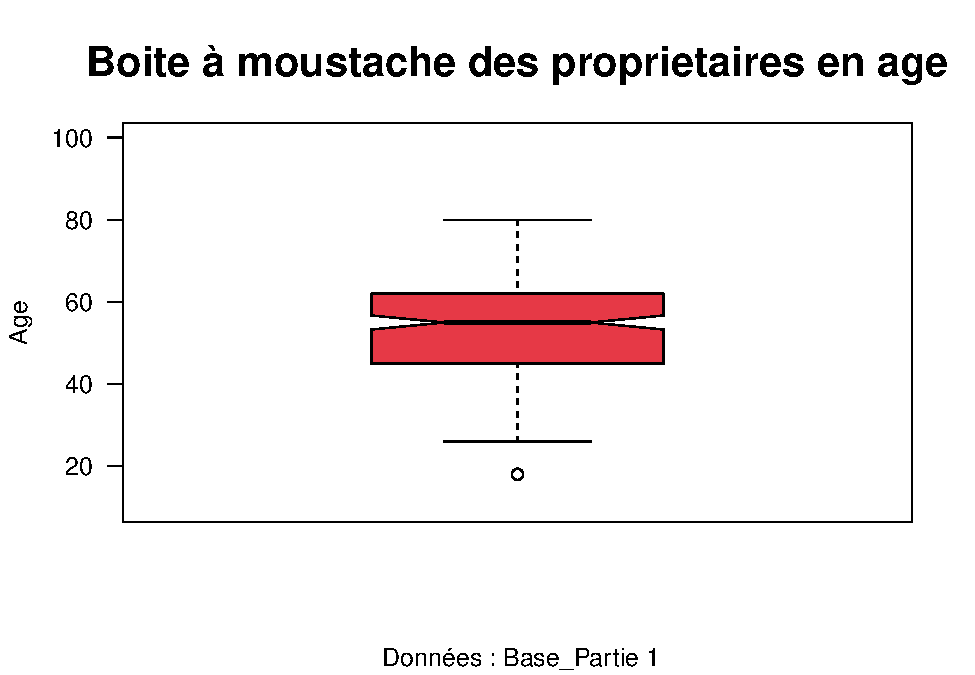
\includegraphics{PROJET_files/figure-latex/unnamed-chunk-21-1.pdf}

\begin{Shaded}
\begin{Highlighting}[]
\CommentTok{\#{-}{-}{-}{-}{-}{-}{-}{-}{-}{-}{-}{-}{-}{-}{-}{-}{-}{-}{-}{-}{-}{-}{-}{-}{-}{-}{-}{-}{-}{-}{-}{-}{-}{-}{-}{-}{-}{-}{-}{-}{-}{-}{-}{-}{-}{-}{-}{-}{-}{-}{-}{-}{-}{-}{-}{-}{-}{-}{-}{-}{-}{-}{-}{-}{-}{-}{-}{-}{-}{-}{-}{-}{-}{-}{-}{-}{-}{-}{-}{-}{-}{-}{-}{-}{-}{-}}
\end{Highlighting}
\end{Shaded}

\begin{Shaded}
\begin{Highlighting}[]
\CommentTok{\#{-}{-}{-}{-}{-}{-}{-}{-}{-}{-}{-}{-}{-}{-}{-}{-}{-}{-}{-}{-}{-}{-}{-}{-}{-}{-}{-}{-}{-}{-}{-}{-}{-}{-}{-}{-}{-}{-}{-}{-}{-}{-}{-}{-}{-}{-}{-}{-}{-}{-}{-}{-}{-}{-}{-}{-}{-}{-}{-}{-}{-}{-}{-}{-}{-}{-}{-}{-}{-}{-}{-}{-}{-}{-}{-}{-}{-}{-}{-}{-}{-}{-}{-}{-}{-}{-}}
\CommentTok{\# Le package ggpirate qui permet de visualiser la distrubition d\textquotesingle{}une maniere plus clair}
\CommentTok{\#{-}{-}{-}{-}{-}{-}{-}{-}{-}{-}{-}{-}{-}{-}{-}{-}{-}{-}{-}{-}{-}{-}{-}{-}{-}{-}{-}{-}{-}{-}{-}{-}{-}{-}{-}{-}{-}{-}{-}{-}{-}{-}{-}{-}{-}{-}{-}{-}{-}{-}{-}{-}{-}{-}{-}{-}{-}{-}{-}{-}{-}{-}{-}{-}{-}{-}{-}{-}{-}{-}{-}{-}{-}{-}{-}{-}{-}{-}{-}{-}{-}{-}{-}{-}{-}}

\NormalTok{Repartition1 }\OtherTok{=}\NormalTok{ projet }\SpecialCharTok{\%\textgreater{}\%}
  
  \FunctionTok{rename}\NormalTok{(}\AttributeTok{age =}\NormalTok{ q24) }\SpecialCharTok{\%\textgreater{}\%} 
  
  \FunctionTok{filter}\NormalTok{( age }\SpecialCharTok{\textless{}} \DecValTok{120}\NormalTok{ )}


\NormalTok{Repartition2 }\OtherTok{=}\NormalTok{ projet }\SpecialCharTok{\%\textgreater{}\%}
  
  \FunctionTok{rename}\NormalTok{(}\AttributeTok{Annees\_experience =}\NormalTok{ q26) }\SpecialCharTok{\%\textgreater{}\%} 
  
  \FunctionTok{filter}\NormalTok{( Annees\_experience }\SpecialCharTok{\textless{}} \DecValTok{50}\NormalTok{ )}


\NormalTok{plot1 }\OtherTok{\textless{}{-}} \FunctionTok{ggplot}\NormalTok{(Repartition1, }\FunctionTok{aes}\NormalTok{(}\AttributeTok{x =}\NormalTok{ sexe, }\AttributeTok{y =}\NormalTok{ age)) }\SpecialCharTok{+}
  
  \FunctionTok{geom\_pirate}\NormalTok{(}\FunctionTok{aes}\NormalTok{(}\AttributeTok{colour =}\NormalTok{ sexe)) }\SpecialCharTok{+}
  
  \FunctionTok{xlab}\NormalTok{(}\StringTok{"Sexe"}\NormalTok{) }\SpecialCharTok{+}
  
  \FunctionTok{ylab}\NormalTok{(}\StringTok{"Âge"}\NormalTok{) }\SpecialCharTok{+}
  
  \FunctionTok{ggtitle}\NormalTok{(}\StringTok{"Répartition par âge selon le sexe"}\NormalTok{) }\SpecialCharTok{+}
  
  \FunctionTok{theme\_light}\NormalTok{()}\SpecialCharTok{+}
  
  \FunctionTok{theme}\NormalTok{(}
    \AttributeTok{plot.title =} \FunctionTok{element\_text}\NormalTok{(}\AttributeTok{color =} \StringTok{"blue"}\NormalTok{))}

\NormalTok{plot2}\OtherTok{\textless{}{-}} \FunctionTok{ggplot}\NormalTok{(Repartition2, }\FunctionTok{aes}\NormalTok{(}\AttributeTok{x =}\NormalTok{ sexe, }\AttributeTok{y =}\NormalTok{ Annees\_experience)) }\SpecialCharTok{+}
  
  \FunctionTok{geom\_pirate}\NormalTok{(}\FunctionTok{aes}\NormalTok{(}\AttributeTok{colour =}\NormalTok{ sexe)) }\SpecialCharTok{+}
  
  \FunctionTok{xlab}\NormalTok{(}\StringTok{"Sexe"}\NormalTok{) }\SpecialCharTok{+}
  
  \FunctionTok{ylab}\NormalTok{(}\StringTok{"Nombre d\textquotesingle{}années d\textquotesingle{}expérience"}\NormalTok{) }\SpecialCharTok{+}
  
  \FunctionTok{ggtitle}\NormalTok{(}\StringTok{"Années d\textquotesingle{}expérience selon le sexe"}\NormalTok{) }\SpecialCharTok{+}
  
  \FunctionTok{theme\_light}\NormalTok{()}\SpecialCharTok{+}
  
  \FunctionTok{theme}\NormalTok{(}
    \AttributeTok{plot.title =} \FunctionTok{element\_text}\NormalTok{(}\AttributeTok{color =} \StringTok{"blue"}\NormalTok{))}

\CommentTok{\# {-}{-}{-}{-}{-}{-}{-}{-}{-}{-}{-}{-}{-}{-}{-}{-}{-}{-}{-}{-}{-}{-}{-}{-}{-}{-}{-}{-}{-}{-}{-}{-}{-}{-}{-}{-}{-}{-}{-}{-}{-}{-}{-}{-}{-}{-}{-}{-}{-}{-}{-}{-}{-}{-}{-}{-}{-}{-}{-}{-}{-}{-}{-}{-}{-}{-}{-}{-}{-}{-}{-}{-}{-}{-}{-}{-}{-}{-}{-}{-}{-}{-}}
\CommentTok{\#Afficher les graphiques côte à côte sur une même ligne}
\CommentTok{\#{-}{-}{-}{-}{-}{-}{-}{-}{-}{-}{-}{-}{-}{-}{-}{-}{-}{-}{-}{-}{-}{-}{-}{-}{-}{-}{-}{-}{-}{-}{-}{-}{-}{-}{-}{-}{-}{-}{-}{-}{-}{-}{-}{-}{-}{-}{-}{-}{-}{-}{-}{-}{-}{-}{-}{-}{-}{-}{-}{-}{-}{-}{-}{-}{-}{-}{-}{-}{-}{-}{-}{-}{-}{-}{-}{-}{-}{-}{-}{-}{-}{-}}

\FunctionTok{grid.arrange}\NormalTok{(plot1, plot2, }\AttributeTok{ncol =} \DecValTok{2}\NormalTok{)}
\end{Highlighting}
\end{Shaded}

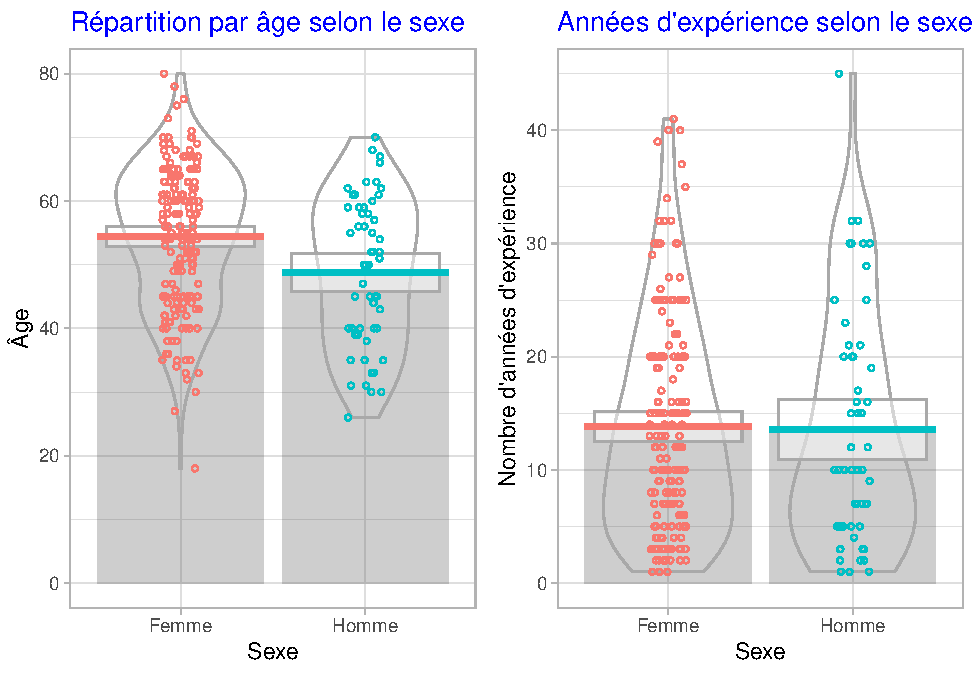
\includegraphics{PROJET_files/figure-latex/unnamed-chunk-22-1.pdf}

\begin{Shaded}
\begin{Highlighting}[]
\CommentTok{\#{-}{-}{-}{-}{-}{-}{-}{-}{-}{-}{-}{-}{-}{-}{-}{-}{-}{-}{-}{-}{-}{-}{-}{-}{-}{-}{-}{-}{-}{-}{-}{-}{-}{-}{-}{-}{-}{-}{-}{-}{-}{-}{-}{-}{-}{-}{-}{-}{-}{-}{-}{-}{-}{-}{-}{-}{-}{-}{-}{-}{-}{-}{-}{-}{-}{-}{-}{-}{-}{-}{-}{-}{-}{-}{-}{-}{-}{-}{-}}
\end{Highlighting}
\end{Shaded}

\newpage

\textcolor{blue}{\subsection{ Transformer le data.frame en données géographiques dont l’objet sera nommé projet\_map}}

\begin{Shaded}
\begin{Highlighting}[]
\CommentTok{\#{-}{-}{-}{-}{-}{-}{-}{-}{-}{-}{-}{-}{-}{-}{-}{-}{-}{-}{-}{-}{-}{-}{-}{-}{-}{-}{-}{-}{-}{-}{-}{-}{-}{-}{-}{-}{-}{-}{-}{-}{-}{-}{-}{-}{-}{-}{-}{-}{-}{-}{-}{-}{-}{-}{-}{-}{-}{-}{-}{-}{-}{-}{-}{-}{-}{-}{-}{-}{-}{-}{-}{-}{-}{-}{-}{-}{-}{-}{-}{-}{-}{-}{-}{-}{-}{-}{-}{-}}
\CommentTok{\# Importation de la base senegal qui contient les coordonnees geographiques au niveau 1 (les regions)}
\CommentTok{\#{-}{-}{-}{-}{-}{-}{-}{-}{-}{-}{-}{-}{-}{-}{-}{-}{-}{-}{-}{-}{-}{-}{-}{-}{-}{-}{-}{-}{-}{-}{-}{-}{-}{-}{-}{-}{-}{-}{-}{-}{-}{-}{-}{-}{-}{-}{-}{-}{-}{-}{-}{-}{-}{-}{-}{-}{-}{-}{-}{-}{-}{-}{-}{-}{-}{-}{-}{-}{-}{-}{-}{-}{-}{-}{-}{-}{-}{-}{-}{-}{-}{-}{-}{-}{-}{-}{-}}

\NormalTok{senegal }\OtherTok{\textless{}{-}} \FunctionTok{st\_read}\NormalTok{(}\StringTok{"SEN\_adm1.shp"}\NormalTok{, }\AttributeTok{layer =} \StringTok{"SEN\_adm1"}\NormalTok{, }\AttributeTok{stringsAsFactors =} \ConstantTok{FALSE}\NormalTok{)}
\end{Highlighting}
\end{Shaded}

\begin{verbatim}
## Reading layer `SEN_adm1' from data source 
##   `C:\Users\medeh\Documents\Projet_R\SEN_adm1.shp' using driver `ESRI Shapefile'
## Simple feature collection with 14 features and 9 fields
## Geometry type: MULTIPOLYGON
## Dimension:     XY
## Bounding box:  xmin: -17.54319 ymin: 12.30786 xmax: -11.34247 ymax: 16.69207
## Geodetic CRS:  WGS 84
\end{verbatim}

\begin{Shaded}
\begin{Highlighting}[]
\CommentTok{\#{-}{-}{-}{-}{-}{-}{-}{-}{-}{-}{-}{-}{-}{-}{-}{-}{-}{-}{-}{-}{-}{-}{-}{-}{-}{-}{-}{-}{-}{-}{-}{-}{-}{-}{-}{-}{-}{-}{-}{-}{-}{-}{-}{-}{-}{-}{-}{-}{-}{-}{-}{-}{-}{-}{-}{-}{-}{-}{-}{-}{-}{-}{-}{-}{-}{-}{-}{-}{-}{-}{-}{-}{-}{-}{-}{-}{-}{-}{-}{-}{-}{-}{-}{-}{-}{-}}
\CommentTok{\#   Creer la variable ID qui prend les regions et selection de ID et les coordonnees geometry}
\CommentTok{\#{-}{-}{-}{-}{-}{-}{-}{-}{-}{-}{-}{-}{-}{-}{-}{-}{-}{-}{-}{-}{-}{-}{-}{-}{-}{-}{-}{-}{-}{-}{-}{-}{-}{-}{-}{-}{-}{-}{-}{-}{-}{-}{-}{-}{-}{-}{-}{-}{-}{-}{-}{-}{-}{-}{-}{-}{-}{-}{-}{-}{-}{-}{-}{-}{-}{-}{-}{-}{-}{-}{-}{-}{-}{-}{-}{-}{-}{-}{-}{-}{-}{-}{-}{-}{-}{-}}

\NormalTok{senegal}\SpecialCharTok{$}\NormalTok{ID }\OtherTok{\textless{}{-}}\NormalTok{ senegal}\SpecialCharTok{$}\NormalTok{NAME\_1}
\NormalTok{senegal }\OtherTok{\textless{}{-}}\NormalTok{ senegal[,}\FunctionTok{c}\NormalTok{(}\DecValTok{11}\NormalTok{,}\DecValTok{10}\NormalTok{)]}


\CommentTok{\#{-}{-}{-}{-}{-}{-}{-}{-}{-}{-}{-}{-}{-}{-}{-}{-}{-}{-}{-}{-}{-}{-}{-}{-}{-}{-}{-}{-}{-}{-}{-}{-}{-}{-}{-}{-}{-}{-}{-}{-}{-}{-}{-}{-}{-}{-}{-}{-}{-}{-}{-}{-}{-}{-}{-}{-}{-}{-}{-}{-}{-}{-}{-}{-}{-}{-}{-}{-}{-}{-}{-}{-}{-}{-}{-}{-}{-}{-}{-}{-}{-}{-}{-}{-}{-}{-}}
\CommentTok{\# Transformation de notre base en donnnes geometrique et specificer crs = st\_crs(senegal)}
\CommentTok{\#{-}{-}{-}{-}{-}{-}{-}{-}{-}{-}{-}{-}{-}{-}{-}{-}{-}{-}{-}{-}{-}{-}{-}{-}{-}{-}{-}{-}{-}{-}{-}{-}{-}{-}{-}{-}{-}{-}{-}{-}{-}{-}{-}{-}{-}{-}{-}{-}{-}{-}{-}{-}{-}{-}{-}{-}{-}{-}{-}{-}{-}{-}{-}{-}{-}{-}{-}{-}{-}{-}{-}{-}{-}{-}{-}{-}{-}{-}{-}{-}{-}{-}{-}{-}{-}{-}}
\NormalTok{projet\_map }\OtherTok{\textless{}{-}} \FunctionTok{st\_as\_sf}\NormalTok{(projet, }\AttributeTok{coords =} \FunctionTok{c}\NormalTok{(}\StringTok{"gps\_menlongitude"}\NormalTok{, }\StringTok{"gps\_menlatitude"}\NormalTok{),}
                       \AttributeTok{crs =} \FunctionTok{st\_crs}\NormalTok{(senegal))}


\NormalTok{projet\_map }\OtherTok{\textless{}{-}} \FunctionTok{st\_join}\NormalTok{(projet\_map,senegal)}

\CommentTok{\#{-}{-}{-}{-}{-}{-}{-}{-}{-}{-}{-}{-}{-}{-}{-}{-}{-}{-}{-}{-}{-}{-}{-}{-}{-}{-}{-}{-}{-}{-}{-}{-}{-}{-}{-}{-}{-}{-}{-}{-}{-}{-}{-}{-}{-}{-}{-}{-}{-}{-}{-}{-}{-}{-}{-}{-}{-}{-}{-}{-}{-}{-}{-}{-}{-}{-}{-}{-}{-}{-}{-}{-}{-}{-}{-}{-}{-}{-}{-}{-}{-}{-}{-}{-}{-}{-}{-}}
\CommentTok{\#             S\textquotesingle{}assurer qu\textquotesingle{}il s\textquotesingle{}agit d\textquotesingle{}un sf}
\CommentTok{\#{-}{-}{-}{-}{-}{-}{-}{-}{-}{-}{-}{-}{-}{-}{-}{-}{-}{-}{-}{-}{-}{-}{-}{-}{-}{-}{-}{-}{-}{-}{-}{-}{-}{-}{-}{-}{-}{-}{-}{-}{-}{-}{-}{-}{-}{-}{-}{-}{-}{-}{-}{-}{-}{-}{-}{-}{-}{-}{-}{-}{-}{-}{-}{-}{-}{-}{-}{-}{-}{-}{-}{-}{-}{-}{-}{-}{-}{-}{-}{-}{-}{-}{-}{-}{-}{-}{-}}
\FunctionTok{class}\NormalTok{(projet\_map)}
\end{Highlighting}
\end{Shaded}

\begin{verbatim}
## [1] "sf"         "tbl_df"     "tbl"        "data.frame"
\end{verbatim}

\begin{Shaded}
\begin{Highlighting}[]
\CommentTok{\#{-}{-}{-}{-}{-}{-}{-}{-}{-}{-}{-}{-}{-}{-}{-}{-}{-}{-}{-}{-}{-}{-}{-}{-}{-}{-}{-}{-}{-}{-}{-}{-}{-}{-}{-}{-}{-}{-}{-}{-}{-}{-}{-}{-}{-}{-}{-}{-}{-}{-}{-}{-}{-}{-}{-}{-}{-}{-}{-}{-}{-}{-}{-}{-}{-}{-}{-}{-}{-}{-}{-}{-}{-}{-}{-}{-}{-}{-}{-}{-}{-}{-}{-}{-}{-}{-}{-}}
\CommentTok{\#  Representation de la carte avec geom\_sf : on represente d\textquotesingle{}abord la carte du senegal }
\CommentTok{\#      comme premiere couche avec la base sebegal}
\CommentTok{\#        Ensuite les coorddones de nos PME avec quelques esthetique pour la beaute}
\CommentTok{\#{-}{-}{-}{-}{-}{-}{-}{-}{-}{-}{-}{-}{-}{-}{-}{-}{-}{-}{-}{-}{-}{-}{-}{-}{-}{-}{-}{-}{-}{-}{-}{-}{-}{-}{-}{-}{-}{-}{-}{-}{-}{-}{-}{-}{-}{-}{-}{-}{-}{-}{-}{-}{-}{-}{-}{-}{-}{-}{-}{-}{-}{-}{-}{-}{-}{-}{-}{-}{-}{-}{-}{-}{-}{-}{-}{-}{-}{-}{-}{-}{-}{-}{-}}

\FunctionTok{ggplot}\NormalTok{() }\SpecialCharTok{+}
  
  \FunctionTok{geom\_sf}\NormalTok{(}\AttributeTok{data =}\NormalTok{ senegal, }\AttributeTok{fill =} \StringTok{"\#CFF183"}\NormalTok{) }\SpecialCharTok{+}
  
  \FunctionTok{geom\_sf}\NormalTok{(}\AttributeTok{data =}\NormalTok{ projet\_map, }\AttributeTok{size =} \DecValTok{2}\NormalTok{, }\FunctionTok{aes}\NormalTok{(}\AttributeTok{fill =}\NormalTok{ sexe, }\AttributeTok{col =}\NormalTok{ sexe, }\AttributeTok{shape =}\NormalTok{ sexe)) }\SpecialCharTok{+}
  
  \FunctionTok{geom\_sf\_text}\NormalTok{(}\AttributeTok{data =}\NormalTok{ senegal, }\FunctionTok{aes}\NormalTok{(}\AttributeTok{label =}\NormalTok{ ID), }\AttributeTok{vjust =} \SpecialCharTok{{-}}\FloatTok{0.5}\NormalTok{, }
               \AttributeTok{check\_overlap =} \ConstantTok{TRUE}\NormalTok{, }\AttributeTok{fontface =} \StringTok{"italic"}\NormalTok{, }\AttributeTok{color =} \StringTok{"black"}\NormalTok{) }\SpecialCharTok{+}
  
  \FunctionTok{labs}\NormalTok{(}\AttributeTok{title =} \StringTok{"REPRESENTATION SPACIALE DES PME PAR SEXE"}\NormalTok{)}\SpecialCharTok{+}
  
  \FunctionTok{theme\_void}\NormalTok{()}\SpecialCharTok{+}
  
   \FunctionTok{theme}\NormalTok{(}
    \AttributeTok{panel.background =} \FunctionTok{element\_rect}\NormalTok{(}\AttributeTok{fill =} \StringTok{"\#ECF1FA"}\NormalTok{), }
      \CommentTok{\# Ajouter une couleur de fond}
    
    \AttributeTok{plot.title =} \FunctionTok{element\_text}\NormalTok{(}\AttributeTok{color =} \StringTok{"\#1E4380"}\NormalTok{, }\AttributeTok{size =} \DecValTok{16}\NormalTok{, }\AttributeTok{face =} \StringTok{"bold"}\NormalTok{),}
    \AttributeTok{legend.position =} \StringTok{"right"}\NormalTok{,}
    
    \AttributeTok{legend.title =} \FunctionTok{element\_text}\NormalTok{(}\AttributeTok{size =} \DecValTok{14}\NormalTok{),}
    
    \AttributeTok{legend.text =} \FunctionTok{element\_text}\NormalTok{(}\AttributeTok{size =} \DecValTok{12}\NormalTok{),}
    
    \AttributeTok{legend.background =} \FunctionTok{element\_rect}\NormalTok{(}\AttributeTok{fill =} \StringTok{"\#ECF1FA"}\NormalTok{, }\AttributeTok{color =} \StringTok{"white"}\NormalTok{),}
    
    \AttributeTok{legend.key =} \FunctionTok{element\_rect}\NormalTok{(}\AttributeTok{color =} \StringTok{"white"}\NormalTok{),}
    
    \AttributeTok{axis.text =} \FunctionTok{element\_text}\NormalTok{(}\AttributeTok{color =} \StringTok{"\#1E4380"}\NormalTok{, }\AttributeTok{size =} \DecValTok{10}\NormalTok{),}
    
    \AttributeTok{axis.title =} \FunctionTok{element\_text}\NormalTok{(}\AttributeTok{color =} \StringTok{"\#1E4380"}\NormalTok{, }\AttributeTok{size =} \DecValTok{12}\NormalTok{)}
\NormalTok{  )}\SpecialCharTok{+}
  
  \FunctionTok{annotation\_scale}\NormalTok{( }\AttributeTok{location =} \StringTok{"bl"}\NormalTok{,}\AttributeTok{width\_hint =} \FloatTok{0.1}\NormalTok{,}
                    
  \AttributeTok{text\_col =} \StringTok{"\#1E4380"}\NormalTok{,}\AttributeTok{text\_size =} \DecValTok{1}\NormalTok{, }\AttributeTok{bar\_col =} \StringTok{"back"}\NormalTok{)}\SpecialCharTok{+}
  
    \FunctionTok{annotation\_north\_arrow}\NormalTok{(}\AttributeTok{location =} \StringTok{"tl"}\NormalTok{, }\AttributeTok{which\_north =} \StringTok{"true"}\NormalTok{,}
                         \AttributeTok{heigt =} \FunctionTok{unit}\NormalTok{(}\FloatTok{0.05}\NormalTok{,}\StringTok{"npc"}\NormalTok{),}\AttributeTok{width =} \FunctionTok{unit}\NormalTok{(}\FloatTok{0.05}\NormalTok{,}\StringTok{"npc"}\NormalTok{))}
\end{Highlighting}
\end{Shaded}

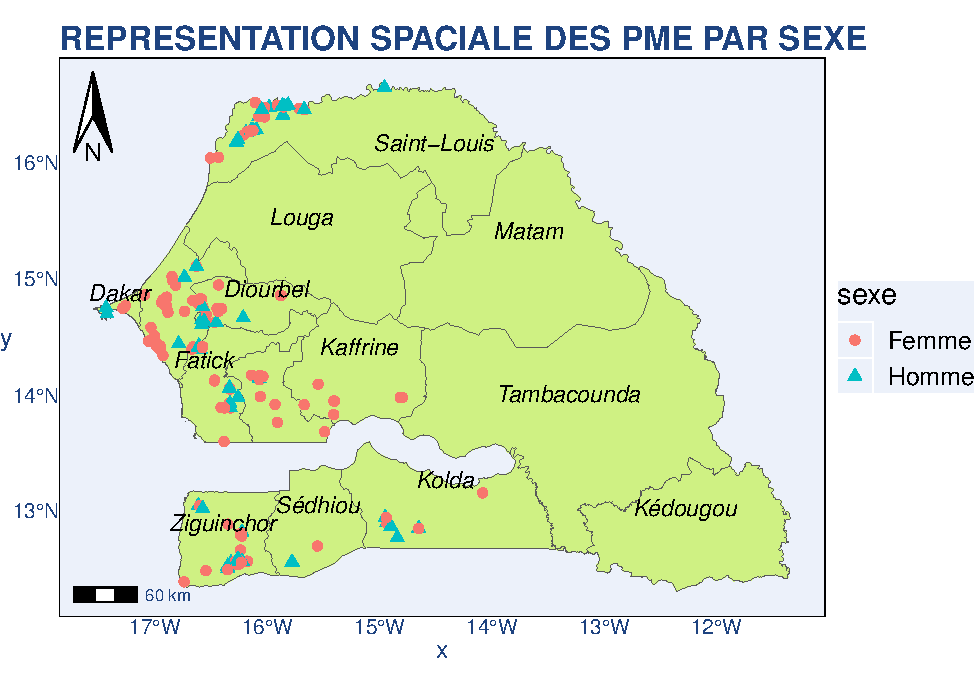
\includegraphics{PROJET_files/figure-latex/unnamed-chunk-23-1.pdf}

\newpage

\textcolor{blue}{\subsection{ La réprésentation spatiale des PME suivant le niveau d’instruction}}

\begin{Shaded}
\begin{Highlighting}[]
\CommentTok{\#{-}{-}{-}{-}{-}{-}{-}{-}{-}{-}{-}{-}{-}{-}{-}{-}{-}{-}{-}{-}{-}{-}{-}{-}{-}{-}{-}{-}{-}{-}{-}{-}{-}{-}{-}{-}{-}{-}{-}{-}{-}{-}{-}{-}{-}{-}{-}{-}{-}{-}{-}{-}{-}{-}{-}{-}{-}{-}{-}{-}{-}{-}{-}{-}{-}{-}{-}{-}{-}{-}{-}{-}{-}{-}{-}{-}{-}{-}{-}{-}{-}{-}{-}{-}{-}{-}{-}}
\CommentTok{\#   Le même jeu que le precedent}
\CommentTok{\#{-}{-}{-}{-}{-}{-}{-}{-}{-}{-}{-}{-}{-}{-}{-}{-}{-}{-}{-}{-}{-}{-}{-}{-}{-}{-}{-}{-}{-}{-}{-}{-}{-}{-}{-}{-}{-}{-}{-}{-}{-}{-}{-}{-}{-}{-}{-}{-}{-}{-}{-}{-}{-}{-}{-}{-}{-}{-}{-}{-}{-}{-}{-}{-}{-}{-}{-}{-}{-}{-}{-}{-}{-}{-}{-}{-}{-}{-}{-}{-}{-}{-}{-}{-}{-}{-}{-}}

\NormalTok{projet\_map }\OtherTok{=}\NormalTok{ projet\_map }\SpecialCharTok{\%\textgreater{}\%} \FunctionTok{rename}\NormalTok{(}\AttributeTok{Niveau\_Instruction =}\NormalTok{ q25)}

\FunctionTok{ggplot}\NormalTok{() }\SpecialCharTok{+}
  
  \FunctionTok{geom\_sf}\NormalTok{(}\AttributeTok{data =}\NormalTok{ senegal, }\AttributeTok{fill =} \StringTok{"\#E8FCEA"}\NormalTok{) }\SpecialCharTok{+}
  
  \FunctionTok{geom\_sf}\NormalTok{(}\AttributeTok{data =}\NormalTok{ projet\_map, }\AttributeTok{size =} \DecValTok{2}\NormalTok{, }\FunctionTok{aes}\NormalTok{(}\AttributeTok{fill =}
\NormalTok{                                             Niveau\_Instruction, }\AttributeTok{col =}\NormalTok{ Niveau\_Instruction, }\AttributeTok{shape =}
\NormalTok{                                             Niveau\_Instruction)) }\SpecialCharTok{+}
  
  \FunctionTok{geom\_sf\_text}\NormalTok{(}\AttributeTok{data =}\NormalTok{ senegal, }\FunctionTok{aes}\NormalTok{(}\AttributeTok{label =}\NormalTok{ ID),}
               
               \AttributeTok{vjust =} \SpecialCharTok{{-}}\FloatTok{0.5}\NormalTok{, }\AttributeTok{check\_overlap =} \ConstantTok{TRUE}\NormalTok{, }\AttributeTok{fontface =}
                 
                 \StringTok{"italic"}\NormalTok{, }\AttributeTok{color =} \StringTok{"black"}\NormalTok{) }\SpecialCharTok{+}
  
  \FunctionTok{labs}\NormalTok{(}\AttributeTok{title =} \StringTok{"REPRESENTATION PAR NIVEAU D\textquotesingle{}INDTRUCTION"}\NormalTok{)}\SpecialCharTok{+}
  
  \FunctionTok{theme\_void}\NormalTok{()}\SpecialCharTok{+}
  
   \FunctionTok{theme}\NormalTok{(}
     
    \AttributeTok{panel.background =} \FunctionTok{element\_rect}\NormalTok{(}\AttributeTok{fill =} \StringTok{"\#ECF1FA"}\NormalTok{),}
    
    \CommentTok{\# Ajouter une couleur de fond}
    
    \AttributeTok{plot.title =} \FunctionTok{element\_text}\NormalTok{(}\AttributeTok{color =} \StringTok{"\#1E4380"}\NormalTok{, }\AttributeTok{size =} \DecValTok{16}\NormalTok{, }\AttributeTok{face =} \StringTok{"bold"}\NormalTok{),}
    
    \AttributeTok{legend.position =} \StringTok{"right"}\NormalTok{,}
    
    \AttributeTok{legend.title =} \FunctionTok{element\_text}\NormalTok{(}\AttributeTok{size =} \DecValTok{14}\NormalTok{),}
    
    \AttributeTok{legend.text =} \FunctionTok{element\_text}\NormalTok{(}\AttributeTok{size =} \DecValTok{12}\NormalTok{),}
    
    \AttributeTok{legend.background =} \FunctionTok{element\_rect}\NormalTok{(}\AttributeTok{fill =} \StringTok{"\#ECF1FA"}\NormalTok{, }\AttributeTok{color =} \StringTok{"white"}\NormalTok{),}
    
    \AttributeTok{legend.key =} \FunctionTok{element\_rect}\NormalTok{(}\AttributeTok{color =} \StringTok{"white"}\NormalTok{),}
    
    \AttributeTok{axis.text =} \FunctionTok{element\_text}\NormalTok{(}\AttributeTok{color =} \StringTok{"\#1E4380"}\NormalTok{, }\AttributeTok{size =} \DecValTok{10}\NormalTok{),}
    
    \AttributeTok{axis.title =} \FunctionTok{element\_text}\NormalTok{(}\AttributeTok{color =} \StringTok{"\#1E4380"}\NormalTok{, }\AttributeTok{size =} \DecValTok{12}\NormalTok{)}
\NormalTok{  )}\SpecialCharTok{+}
  
  \FunctionTok{annotation\_scale}\NormalTok{( }\AttributeTok{location =} \StringTok{"bl"}\NormalTok{,}\AttributeTok{width\_hint =} \FloatTok{0.1}\NormalTok{,}
                    
  \AttributeTok{text\_col =} \StringTok{"\#1E4380"}\NormalTok{,}\AttributeTok{text\_size =} \DecValTok{1}\NormalTok{, }\AttributeTok{bar\_col =} \StringTok{"back"}\NormalTok{)}\SpecialCharTok{+}
  
    \FunctionTok{annotation\_north\_arrow}\NormalTok{(}\AttributeTok{location =} \StringTok{"tl"}\NormalTok{, }\AttributeTok{which\_north =}
                             \StringTok{"true"}\NormalTok{,}
                           
                         \AttributeTok{heigt =} \FunctionTok{unit}\NormalTok{(}\FloatTok{0.05}\NormalTok{,}\StringTok{"npc"}\NormalTok{),}\AttributeTok{width =} \FunctionTok{unit}\NormalTok{(}\FloatTok{0.05}\NormalTok{,}\StringTok{"npc"}\NormalTok{))}
\end{Highlighting}
\end{Shaded}

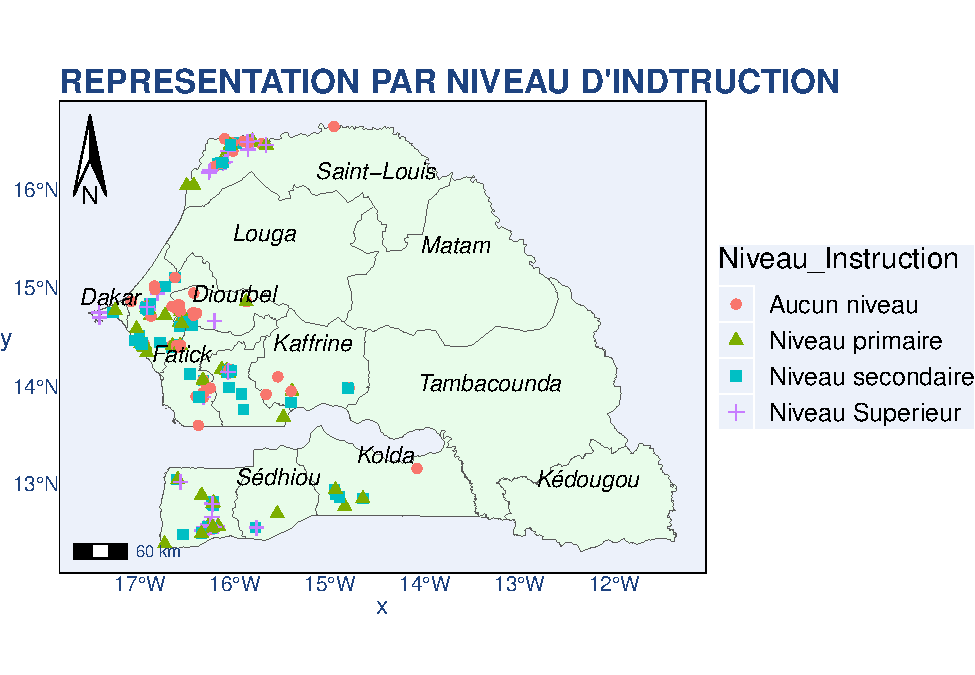
\includegraphics{PROJET_files/figure-latex/unnamed-chunk-24-1.pdf}

\newpage

\textcolor{blue}{\subsection{ Faites une analyse spatiale de votre choix}}

\begin{Shaded}
\begin{Highlighting}[]
\CommentTok{\#{-}{-}{-}{-}{-}{-}{-}{-}{-}{-}{-}{-}{-}{-}{-}{-}{-}{-}{-}{-}{-}{-}{-}{-}{-}{-}{-}{-}{-}{-}{-}{-}{-}{-}{-}{-}{-}{-}{-}{-}{-}{-}{-}{-}{-}{-}{-}{-}{-}{-}{-}{-}{-}{-}{-}{-}{-}{-}{-}{-}{-}{-}{-}{-}{-}{-}{-}{-}{-}{-}{-}{-}{-}{-}{-}{-}{-}{-}{-}{-}{-}{-}{-}{-}{-}{-}{-}}
\CommentTok{\#  Regouper par filiere avec uniquement ceux qui ceux qui sont specialisés dans  }
\CommentTok{\#   les filieres : On a dont 4 tableaux Tab1...Tab2}
\CommentTok{\#{-}{-}{-}{-}{-}{-}{-}{-}{-}{-}{-}{-}{-}{-}{-}{-}{-}{-}{-}{-}{-}{-}{-}{-}{-}{-}{-}{-}{-}{-}{-}{-}{-}{-}{-}{-}{-}{-}{-}{-}{-}{-}{-}{-}{-}{-}{-}{-}{-}{-}{-}{-}{-}{-}{-}{-}{-}{-}{-}{-}{-}{-}{-}{-}{-}{-}{-}{-}{-}{-}{-}{-}{-}{-}{-}{-}{-}{-}{-}{-}{-}{-}{-}{-}{-}{-}{-}{-}}

\NormalTok{Tab1 }\OtherTok{=}\NormalTok{ projet }\SpecialCharTok{\%\textgreater{}\%}
\FunctionTok{filter}\NormalTok{(filiere\_1 }\SpecialCharTok{==} \DecValTok{1}\NormalTok{) }\SpecialCharTok{\%\textgreater{}\%}
\NormalTok{dplyr}\SpecialCharTok{::}\FunctionTok{mutate}\NormalTok{(}\AttributeTok{FILIERE =} \FunctionTok{ifelse}\NormalTok{(filiere\_1 }\SpecialCharTok{==} \DecValTok{1}\NormalTok{, }\StringTok{"Arachide"}\NormalTok{))}


\NormalTok{Tab2 }\OtherTok{=}\NormalTok{ projet }\SpecialCharTok{\%\textgreater{}\%}
  \FunctionTok{filter}\NormalTok{(filiere\_2 }\SpecialCharTok{==} \DecValTok{1}\NormalTok{) }\SpecialCharTok{\%\textgreater{}\%}
\NormalTok{  dplyr}\SpecialCharTok{::}\FunctionTok{mutate}\NormalTok{(}\AttributeTok{Anacarde =} \FunctionTok{ifelse}\NormalTok{(filiere\_2 }\SpecialCharTok{==} \DecValTok{1}\NormalTok{, }\StringTok{"Anacarde"}\NormalTok{))}


\NormalTok{Tab3 }\OtherTok{=}\NormalTok{ projet }\SpecialCharTok{\%\textgreater{}\%}
  \FunctionTok{filter}\NormalTok{(filiere\_3 }\SpecialCharTok{==} \DecValTok{1}\NormalTok{) }\SpecialCharTok{\%\textgreater{}\%}
\NormalTok{  dplyr}\SpecialCharTok{::}\FunctionTok{mutate}\NormalTok{(}\AttributeTok{Mangue =} \FunctionTok{ifelse}\NormalTok{(filiere\_3 }\SpecialCharTok{==} \DecValTok{1}\NormalTok{, }\StringTok{"Mangue"}\NormalTok{))}


\NormalTok{Tab4 }\OtherTok{=}\NormalTok{ projet }\SpecialCharTok{\%\textgreater{}\%}\FunctionTok{filter}\NormalTok{(filiere\_4 }\SpecialCharTok{==} \DecValTok{1}\NormalTok{) }\SpecialCharTok{\%\textgreater{}\%}
\NormalTok{  dplyr}\SpecialCharTok{::}\FunctionTok{mutate}\NormalTok{(}\AttributeTok{Riz =} \FunctionTok{ifelse}\NormalTok{(filiere\_4 }\SpecialCharTok{==} \DecValTok{1}\NormalTok{, }\StringTok{"Riz"}\NormalTok{))}


\CommentTok{\#{-}{-}{-}{-}{-}{-}{-}{-}{-}{-}{-}{-}{-}{-}{-}{-}{-}{-}{-}{-}{-}{-}{-}{-}{-}{-}{-}{-}{-}{-}{-}{-}{-}{-}{-}{-}{-}{-}{-}{-}{-}{-}{-}{-}{-}{-}{-}{-}{-}{-}{-}{-}{-}{-}{-}{-}{-}{-}{-}{-}{-}{-}{-}{-}{-}{-}{-}{-}{-}{-}{-}{-}{-}{-}{-}{-}{-}{-}{-}{-}{-}{-}{-}{-}{-}{-}{-}{-}}
\CommentTok{\# Importation de la base senegal qui contient les coordonnees geographiques }
\CommentTok{\#    au niveau 2 (les departements) }
\CommentTok{\#   Et le même jeu comme les deux carte precedentes}
\CommentTok{\#{-}{-}{-}{-}{-}{-}{-}{-}{-}{-}{-}{-}{-}{-}{-}{-}{-}{-}{-}{-}{-}{-}{-}{-}{-}{-}{-}{-}{-}{-}{-}{-}{-}{-}{-}{-}{-}{-}{-}{-}{-}{-}{-}{-}{-}{-}{-}{-}{-}{-}{-}{-}{-}{-}{-}{-}{-}{-}{-}{-}{-}{-}{-}{-}{-}{-}{-}{-}{-}{-}{-}{-}{-}{-}{-}{-}{-}{-}{-}{-}{-}{-}{-}{-}{-}{-}{-}}

\NormalTok{sene }\OtherTok{\textless{}{-}} \FunctionTok{st\_read}\NormalTok{(}\StringTok{"SEN\_adm2.shp"}\NormalTok{, }\AttributeTok{layer =} \StringTok{"SEN\_adm2"}\NormalTok{, }\AttributeTok{stringsAsFactors =} \ConstantTok{FALSE}\NormalTok{)}
\end{Highlighting}
\end{Shaded}

\begin{verbatim}
## Reading layer `SEN_adm2' from data source 
##   `C:\Users\medeh\Documents\Projet_R\SEN_adm2.shp' using driver `ESRI Shapefile'
## Simple feature collection with 45 features and 11 fields
## Geometry type: MULTIPOLYGON
## Dimension:     XY
## Bounding box:  xmin: -17.54319 ymin: 12.30786 xmax: -11.34247 ymax: 16.69207
## Geodetic CRS:  WGS 84
\end{verbatim}

\begin{Shaded}
\begin{Highlighting}[]
\NormalTok{Tab1 }\OtherTok{\textless{}{-}} \FunctionTok{st\_as\_sf}\NormalTok{(Tab1, }\AttributeTok{coords =} \FunctionTok{c}\NormalTok{(}\StringTok{"gps\_menlongitude"}\NormalTok{, }\StringTok{"gps\_menlatitude"}\NormalTok{), }\AttributeTok{crs =} \FunctionTok{st\_crs}\NormalTok{(sene))}



\NormalTok{Tab2 }\OtherTok{\textless{}{-}} \FunctionTok{st\_as\_sf}\NormalTok{(Tab2, }\AttributeTok{coords =} \FunctionTok{c}\NormalTok{(}\StringTok{"gps\_menlongitude"}\NormalTok{, }\StringTok{"gps\_menlatitude"}\NormalTok{), }\AttributeTok{crs =} \FunctionTok{st\_crs}\NormalTok{(sene))}



\NormalTok{Tab3 }\OtherTok{\textless{}{-}} \FunctionTok{st\_as\_sf}\NormalTok{(Tab3, }\AttributeTok{coords =} \FunctionTok{c}\NormalTok{(}\StringTok{"gps\_menlongitude"}\NormalTok{, }\StringTok{"gps\_menlatitude"}\NormalTok{), }\AttributeTok{crs =} \FunctionTok{st\_crs}\NormalTok{(sene))}



\NormalTok{Tab4 }\OtherTok{\textless{}{-}} \FunctionTok{st\_as\_sf}\NormalTok{(Tab4, }\AttributeTok{coords =} \FunctionTok{c}\NormalTok{(}\StringTok{"gps\_menlongitude"}\NormalTok{, }\StringTok{"gps\_menlatitude"}\NormalTok{), }\AttributeTok{crs =} \FunctionTok{st\_crs}\NormalTok{(sene))}



\NormalTok{Tab1 }\OtherTok{\textless{}{-}} \FunctionTok{st\_join}\NormalTok{(Tab1,sene)}
\NormalTok{Tab2 }\OtherTok{\textless{}{-}} \FunctionTok{st\_join}\NormalTok{(Tab2,sene)}
\NormalTok{Tab3 }\OtherTok{\textless{}{-}} \FunctionTok{st\_join}\NormalTok{(Tab3,sene)}
\NormalTok{Tab4 }\OtherTok{\textless{}{-}} \FunctionTok{st\_join}\NormalTok{(Tab4,sene)}



\FunctionTok{ggplot}\NormalTok{() }\SpecialCharTok{+}
  
  \FunctionTok{geom\_sf}\NormalTok{(}\AttributeTok{data =}\NormalTok{ sene, }\AttributeTok{fill =} \StringTok{"\#FEFBEC"}\NormalTok{) }\SpecialCharTok{+}
  
  \FunctionTok{geom\_sf}\NormalTok{(}\AttributeTok{data =}\NormalTok{ Tab1, }\AttributeTok{size =} \DecValTok{2}\NormalTok{, }\FunctionTok{aes}\NormalTok{(}\AttributeTok{fill =}\NormalTok{ FILIERE, }\AttributeTok{col =}\NormalTok{ FILIERE , }\AttributeTok{shape =}\NormalTok{ FILIERE  ))}\SpecialCharTok{+}
  
  \FunctionTok{geom\_sf}\NormalTok{(}\AttributeTok{data =}\NormalTok{ Tab2, }\AttributeTok{size =} \DecValTok{2}\NormalTok{, }\FunctionTok{aes}\NormalTok{(}\AttributeTok{fill =}\NormalTok{ Anacarde,}\AttributeTok{col =}\NormalTok{ Anacarde,}\AttributeTok{shape =}\NormalTok{ Anacarde))}\SpecialCharTok{+}
  
  \FunctionTok{geom\_sf}\NormalTok{(}\AttributeTok{data =}\NormalTok{ Tab3, }\AttributeTok{size =} \DecValTok{2}\NormalTok{, }\FunctionTok{aes}\NormalTok{(}\AttributeTok{fill =}\NormalTok{ Mangue,}\AttributeTok{col =}\NormalTok{ Mangue,}\AttributeTok{shape =}\NormalTok{ Mangue))}\SpecialCharTok{+}
  
  \FunctionTok{geom\_sf}\NormalTok{(}\AttributeTok{data =}\NormalTok{ Tab4, }\AttributeTok{size =} \DecValTok{2}\NormalTok{, }\FunctionTok{aes}\NormalTok{(}\AttributeTok{fill =}\NormalTok{ Riz,}\AttributeTok{col =}\NormalTok{ Riz, }\AttributeTok{shape =}\NormalTok{ Riz))}\SpecialCharTok{+}
  
  \FunctionTok{geom\_sf\_text}\NormalTok{(}\AttributeTok{data =}\NormalTok{ sene, }\FunctionTok{aes}\NormalTok{(}\AttributeTok{label =}\NormalTok{ NAME\_2),}
               \AttributeTok{vjust =} \SpecialCharTok{{-}}\FloatTok{0.1}\NormalTok{, }\AttributeTok{check\_overlap =} \ConstantTok{TRUE}\NormalTok{, }\AttributeTok{fontface =} \StringTok{"italic"}\NormalTok{, }\AttributeTok{color =} \StringTok{"black"}\NormalTok{) }\SpecialCharTok{+}
  
  \FunctionTok{labs}\NormalTok{(}\AttributeTok{title =} \StringTok{"LES FILIERES PAR DEPARTEMENT"}\NormalTok{)}\SpecialCharTok{+}
  
  \FunctionTok{theme\_void}\NormalTok{()}\SpecialCharTok{+}
  
   \FunctionTok{theme}\NormalTok{(}
    \AttributeTok{panel.background =} \FunctionTok{element\_rect}\NormalTok{(}\AttributeTok{fill =} \StringTok{"\#ECF1FA"}\NormalTok{),  }\CommentTok{\# Ajouter une couleur de fond}
    \AttributeTok{plot.title =} \FunctionTok{element\_text}\NormalTok{(}\AttributeTok{color =} \StringTok{"\#1E4380"}\NormalTok{, }\AttributeTok{size =} \DecValTok{16}\NormalTok{, }\AttributeTok{face =} \StringTok{"bold"}\NormalTok{),}
    
    \AttributeTok{legend.position =} \StringTok{"right"}\NormalTok{,}
    
    \AttributeTok{legend.title =} \FunctionTok{element\_text}\NormalTok{(}\AttributeTok{size =} \DecValTok{14}\NormalTok{),}
    
    \AttributeTok{legend.text =} \FunctionTok{element\_text}\NormalTok{(}\AttributeTok{size =} \DecValTok{12}\NormalTok{),}
    
    \AttributeTok{legend.background =} \FunctionTok{element\_rect}\NormalTok{(}\AttributeTok{fill =} \StringTok{"\#ECF1FA"}\NormalTok{, }\AttributeTok{color =} \StringTok{"white"}\NormalTok{),}
    
    \AttributeTok{legend.key =} \FunctionTok{element\_rect}\NormalTok{(}\AttributeTok{color =} \StringTok{"white"}\NormalTok{),}
    
    \AttributeTok{axis.text =} \FunctionTok{element\_text}\NormalTok{(}\AttributeTok{color =} \StringTok{"\#1E4380"}\NormalTok{, }\AttributeTok{size =} \DecValTok{10}\NormalTok{),}
    
    \AttributeTok{axis.title =} \FunctionTok{element\_text}\NormalTok{(}\AttributeTok{color =} \StringTok{"\#1E4380"}\NormalTok{, }\AttributeTok{size =} \DecValTok{12}\NormalTok{)}
\NormalTok{  )}\SpecialCharTok{+}
  
  \FunctionTok{annotation\_scale}\NormalTok{( }\AttributeTok{location =} \StringTok{"bl"}\NormalTok{,}\AttributeTok{width\_hint =} \FloatTok{0.1}\NormalTok{,}
                    
  \AttributeTok{text\_col =} \StringTok{"\#1E4380"}\NormalTok{,}\AttributeTok{text\_size =} \DecValTok{1}\NormalTok{, }\AttributeTok{bar\_col =} \StringTok{"back"}\NormalTok{)}\SpecialCharTok{+}
  
    \FunctionTok{annotation\_north\_arrow}\NormalTok{(}\AttributeTok{location =} \StringTok{"tl"}\NormalTok{, }\AttributeTok{which\_north =} \StringTok{"true"}\NormalTok{,}
                         \AttributeTok{heigt =} \FunctionTok{unit}\NormalTok{(}\FloatTok{0.05}\NormalTok{,}\StringTok{"npc"}\NormalTok{),}\AttributeTok{width =} \FunctionTok{unit}\NormalTok{(}\FloatTok{0.05}\NormalTok{,}\StringTok{"npc"}\NormalTok{))}
\end{Highlighting}
\end{Shaded}

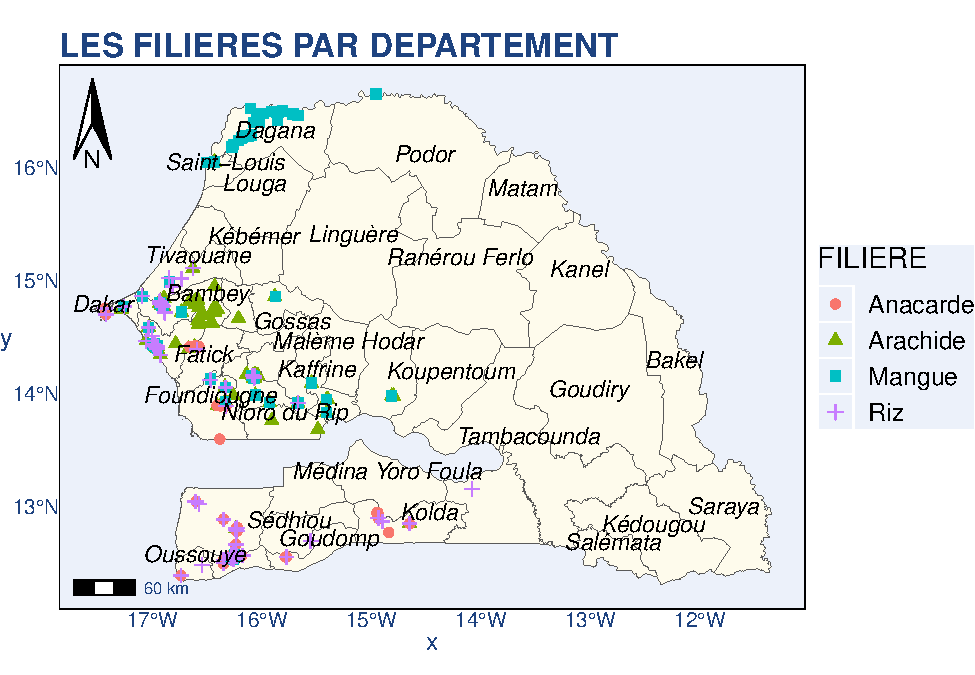
\includegraphics{PROJET_files/figure-latex/unnamed-chunk-25-1.pdf}

\newpage

\textcolor{blue}{\section*{PARTIE II}\addcontentsline{toc}{section}{PARTIE II}}

\textcolor{blue}{\section{Nettoyage et gestion des données}}

\textcolor{blue}{\subsection{ Nomination de la variable country\_destination en destination et définition des valeurs négatives
comme manquantes}}

\begin{Shaded}
\begin{Highlighting}[]
\CommentTok{\#{-}{-}{-}{-}{-}{-}{-}{-}{-}{-}{-}{-}{-}{-}{-}{-}{-}{-}{-}{-}{-}{-}{-}{-}{-}{-}{-}{-}{-}{-}{-}{-}{-}{-}{-}{-}{-}{-}{-}{-}{-}{-}{-}{-}{-}{-}{-}{-}{-}{-}{-}{-}{-}{-}{-}{-}{-}{-}{-}{-}{-}{-}{-}{-}{-}{-}{-}{-}{-}{-}{-}{-}{-}{-}{-}{-}{-}{-}{-}{-}{-}{-}{-}{-}{-}{-}}
\CommentTok{\# lecture de la feuille 1 du fichier Excel "Base\_Partie 2.xlsx" :IMPORTATION  }
\CommentTok{\# Utilisation de la fonction rename pour renommer }
\CommentTok{\#{-}{-}{-}{-}{-}{-}{-}{-}{-}{-}{-}{-}{-}{-}{-}{-}{-}{-}{-}{-}{-}{-}{-}{-}{-}{-}{-}{-}{-}{-}{-}{-}{-}{-}{-}{-}{-}{-}{-}{-}{-}{-}{-}{-}{-}{-}{-}{-}{-}{-}{-}{-}{-}{-}{-}{-}{-}{-}{-}{-}{-}{-}{-}{-}{-}{-}{-}{-}{-}{-}{-}{-}{-}{-}{-}{-}{-}{-}{-}{-}{-}{-}{-}{-}{-}{-}}

\NormalTok{Feuille1 }\OtherTok{\textless{}{-}} \FunctionTok{read\_excel}\NormalTok{(}\StringTok{"Base\_Partie 2.xlsx"}\NormalTok{)}

\NormalTok{Feuille1 }\OtherTok{\textless{}{-}}\NormalTok{ Feuille1 }\SpecialCharTok{\%\textgreater{}\%}
  
\FunctionTok{rename}\NormalTok{(}\AttributeTok{destination =}\NormalTok{ country\_destination) }\SpecialCharTok{\%\textgreater{}\%}
  
\FunctionTok{mutate}\NormalTok{(}\FunctionTok{across}\NormalTok{(}\FunctionTok{everything}\NormalTok{(), }\SpecialCharTok{\textasciitilde{}} \FunctionTok{ifelse}\NormalTok{(. }\SpecialCharTok{\textless{}} \DecValTok{0}\NormalTok{, }\ConstantTok{NA}\NormalTok{, .)))}

\CommentTok{\# ou encore Feuille1[Feuille1 \textless{} 0] \textless{}{-} NA}

\NormalTok{Feuille1 }\SpecialCharTok{\%\textgreater{}\%}
  
  \FunctionTok{head}\NormalTok{()}
\end{Highlighting}
\end{Shaded}

\begin{verbatim}
## # A tibble: 6 x 10
##      id starttime endtime enumerator district   age   sex children_num intention
##   <dbl>     <dbl>   <dbl>      <dbl>    <dbl> <dbl> <dbl>        <dbl>     <dbl>
## 1     2    1.55e9  1.55e9          6        1    33     1            1         1
## 2     3    1.55e9  1.55e9          6        1    43     0            5         1
## 3     4    1.55e9  1.55e9          6        1    28     0            0         1
## 4     7    1.55e9  1.55e9          8        3    24     0            0         1
## 5     8    1.55e9  1.55e9          8        3    29     0            0         1
## 6    10    1.55e9  1.55e9          8        6    22     1            0         1
## # i 1 more variable: destination <dbl>
\end{verbatim}

\begin{Shaded}
\begin{Highlighting}[]
\CommentTok{\#{-}{-}{-}{-}{-}{-}{-}{-}{-}{-}{-}{-}{-}{-}{-}{-}{-}{-}{-}{-}{-}{-}{-}{-}{-}{-}{-}{-}{-}{-}{-}{-}{-}{-}{-}{-}{-}{-}{-}{-}{-}{-}{-}{-}{-}{-}{-}{-}{-}{-}{-}{-}{-}{-}{-}{-}{-}{-}{-}{-}{-}{-}{-}{-}{-}{-}{-}{-}{-}{-}{-}{-}{-}{-}{-}{-}{-}{-}{-}{-}{-}{-}{-}{-}{-}}
\end{Highlighting}
\end{Shaded}

\textcolor{blue}{\subsection{Créer une nouvelle variable contenant des tranches d’âge de 5 ans en utilisant la variable “age”}}

\begin{Shaded}
\begin{Highlighting}[]
\CommentTok{\#{-}{-}{-}{-}{-}{-}{-}{-}{-}{-}{-}{-}{-}{-}{-}{-}{-}{-}{-}{-}{-}{-}{-}{-}{-}{-}{-}{-}{-}{-}{-}{-}{-}{-}{-}{-}{-}{-}{-}{-}{-}{-}{-}{-}{-}{-}{-}{-}{-}{-}{-}{-}{-}{-}{-}{-}{-}{-}{-}{-}{-}{-}{-}{-}{-}{-}{-}{-}{-}{-}{-}{-}{-}{-}{-}{-}{-}{-}{-}{-}{-}{-}{-}{-}{-}{-}{-}}
\CommentTok{\#  1)  Attacher la base }
\CommentTok{\#    Definir un vecteur textlab qui prends les chaines de charactere "[a,b["}
\CommentTok{\#    Creer la nouvelle variables de groupe d\textquotesingle{}age avec cut}

\FunctionTok{attach}\NormalTok{(Feuille1)}

\FunctionTok{min}\NormalTok{(age)}
\end{Highlighting}
\end{Shaded}

\begin{verbatim}
## [1] 15
\end{verbatim}

\begin{Shaded}
\begin{Highlighting}[]
\NormalTok{textlab }\OtherTok{\textless{}{-}}\FunctionTok{c}\NormalTok{()}

\NormalTok{largeur }\OtherTok{\textless{}{-}} \DecValTok{5}

\NormalTok{nbcat }\OtherTok{\textless{}{-}} \DecValTok{9}

\ControlFlowTok{for}\NormalTok{( i }\ControlFlowTok{in} \DecValTok{3} \SpecialCharTok{:}\NormalTok{ (nbcat }\SpecialCharTok{{-}} \DecValTok{1}\NormalTok{ ))\{}
  
\NormalTok{textlab[i}\SpecialCharTok{+}\DecValTok{1}\NormalTok{] }\OtherTok{\textless{}{-}} \FunctionTok{paste}\NormalTok{(}\StringTok{"["}\NormalTok{,}\FunctionTok{as.character}\NormalTok{(i}\SpecialCharTok{*}\NormalTok{largeur),}\StringTok{","}\NormalTok{,}\FunctionTok{as.character}\NormalTok{((i}\SpecialCharTok{+}\DecValTok{1}\NormalTok{)}\SpecialCharTok{*}\NormalTok{largeur),}\StringTok{"["}\NormalTok{,}\AttributeTok{sep=}\StringTok{""}\NormalTok{)\}}

\NormalTok{textlab }\OtherTok{\textless{}{-}}\NormalTok{ textlab[}\FunctionTok{complete.cases}\NormalTok{(textlab)]}
\CommentTok{\# Supprimer les valeur manquantes pour une dimension identique}


\NormalTok{Feuille1 }\OtherTok{=}\NormalTok{ Feuille1 }\SpecialCharTok{\%\textgreater{}\%} 
  
  \FunctionTok{mutate}\NormalTok{( }\AttributeTok{group\_age =} \FunctionTok{cut}\NormalTok{ ( age, }\AttributeTok{breaks =} \FunctionTok{seq}\NormalTok{(}\AttributeTok{from =} \DecValTok{15}\NormalTok{, }\AttributeTok{to =}\NormalTok{ nbcat}\SpecialCharTok{*}\NormalTok{largeur,}
                                              \AttributeTok{by =}\NormalTok{ largeur), }\AttributeTok{labels =}\NormalTok{ textlab),}\AttributeTok{.after =}\NormalTok{ age) }

\NormalTok{Feuille1 }\SpecialCharTok{\%\textgreater{}\%}
  
  \FunctionTok{head}\NormalTok{()}
\end{Highlighting}
\end{Shaded}

\begin{verbatim}
## # A tibble: 6 x 11
##      id starttime endtime enumerator district   age group_age   sex children_num
##   <dbl>     <dbl>   <dbl>      <dbl>    <dbl> <dbl> <fct>     <dbl>        <dbl>
## 1     2    1.55e9  1.55e9          6        1    33 [30,35[       1            1
## 2     3    1.55e9  1.55e9          6        1    43 [40,45[       0            5
## 3     4    1.55e9  1.55e9          6        1    28 [25,30[       0            0
## 4     7    1.55e9  1.55e9          8        3    24 [20,25[       0            0
## 5     8    1.55e9  1.55e9          8        3    29 [25,30[       0            0
## 6    10    1.55e9  1.55e9          8        6    22 [20,25[       1            0
## # i 2 more variables: intention <dbl>, destination <dbl>
\end{verbatim}

\textcolor{blue}{\subsection{Créer une nouvelle variable contenant le nombre d’entretiens réalisés par chaque agent recenseur}}

\begin{Shaded}
\begin{Highlighting}[]
\CommentTok{\#{-}{-}{-}{-}{-}{-}{-}{-}{-}{-}{-}{-}{-}{-}{-}{-}{-}{-}{-}{-}{-}{-}{-}{-}{-}{-}{-}{-}{-}{-}{-}{-}{-}{-}{-}{-}{-}{-}{-}{-}{-}{-}{-}{-}{-}{-}{-}{-}{-}{-}{-}{-}{-}{-}{-}{-}{-}{-}{-}{-}{-}{-}{-}{-}{-}{-}{-}{-}{-}{-}{-}{-}{-}{-}{-}{-}{-}{-}{-}{-}{-}{-}{-}{-}{-}{-}{-}{-}{-}{-}{-}}
\CommentTok{\#   La fonction count pour compter le nombre de repetition de }
\CommentTok{\#   la variable enumerator et l\textquotesingle{}ajouter a la variable nombre\_entretien}
\CommentTok{\#{-}{-}{-}{-}{-}{-}{-}{-}{-}{-}{-}{-}{-}{-}{-}{-}{-}{-}{-}{-}{-}{-}{-}{-}{-}{-}{-}{-}{-}{-}{-}{-}{-}{-}{-}{-}{-}{-}{-}{-}{-}{-}{-}{-}{-}{-}{-}{-}{-}{-}{-}{-}{-}{-}{-}{-}{-}{-}{-}{-}{-}{-}{-}{-}{-}{-}{-}{-}{-}{-}{-}{-}{-}{-}{-}{-}{-}{-}{-}{-}{-}{-}{-}{-}{-}{-}{-}{-}{-}{-}{-}}

\NormalTok{Entretien }\OtherTok{=}\NormalTok{ Feuille1 }\SpecialCharTok{\%\textgreater{}\%}
  
\FunctionTok{count}\NormalTok{(enumerator, }\AttributeTok{sort =} \ConstantTok{TRUE}\NormalTok{ , }\AttributeTok{name =} \StringTok{"nombre\_entretien"}\NormalTok{)}

\NormalTok{Entretien}
\end{Highlighting}
\end{Shaded}

\begin{verbatim}
## # A tibble: 16 x 2
##    enumerator nombre_entretien
##         <dbl>            <int>
##  1          4                9
##  2         20                9
##  3         13                8
##  4          7                7
##  5         11                7
##  6          5                6
##  7          8                6
##  8          9                6
##  9         14                6
## 10         17                6
## 11         18                6
## 12          1                5
## 13          6                5
## 14         10                5
## 15         12                5
## 16         15                1
\end{verbatim}

\textcolor{blue}{\subsection{Créer une nouvelle variable qui affecte aléatoirement chaque répondant à un groupe de traitement (1) ou
de controle (0)}}

\begin{Shaded}
\begin{Highlighting}[]
\CommentTok{\#{-}{-}{-}{-}{-}{-}{-}{-}{-}{-}{-}{-}{-}{-}{-}{-}{-}{-}{-}{-}{-}{-}{-}{-}{-}{-}{-}{-}{-}{-}{-}{-}{-}{-}{-}{-}{-}{-}{-}{-}{-}{-}{-}{-}{-}{-}{-}{-}{-}{-}{-}{-}{-}{-}{-}{-}{-}{-}{-}{-}{-}{-}{-}{-}{-}{-}{-}{-}{-}{-}{-}{-}{-}{-}{-}{-}{-}{-}{-}{-}{-}{-}{-}{-}{-}{-}{-}{-}}
\CommentTok{\#    set.seed pour fixer l\textquotesingle{}alea}
\CommentTok{\#{-}{-}{-}{-}{-}{-}{-}{-}{-}{-}{-}{-}{-}{-}{-}{-}{-}{-}{-}{-}{-}{-}{-}{-}{-}{-}{-}{-}{-}{-}{-}{-}{-}{-}{-}{-}{-}{-}{-}{-}{-}{-}{-}{-}{-}{-}{-}{-}{-}{-}{-}{-}{-}{-}{-}{-}{-}{-}{-}{-}{-}{-}{-}{-}{-}{-}{-}{-}{-}{-}{-}{-}{-}{-}{-}{-}{-}{-}{-}{-}{-}{-}{-}{-}{-}{-}{-}{-}{-}}

\FunctionTok{set.seed}\NormalTok{(}\DecValTok{012}\NormalTok{)}

\NormalTok{Feuille1 }\OtherTok{=}\NormalTok{ Feuille1 }\SpecialCharTok{\%\textgreater{}\%}
  
\FunctionTok{mutate}\NormalTok{( }\AttributeTok{traitement =} \FunctionTok{sample}\NormalTok{(}\FunctionTok{c}\NormalTok{(}\DecValTok{0}\NormalTok{,}\DecValTok{1}\NormalTok{), }\AttributeTok{size =} \FunctionTok{nrow}\NormalTok{(Feuille1), }\AttributeTok{replace =} \ConstantTok{TRUE}\NormalTok{))}


\NormalTok{Feuille1 }\SpecialCharTok{\%\textgreater{}\%}
  
  \FunctionTok{head}\NormalTok{()}
\end{Highlighting}
\end{Shaded}

\begin{verbatim}
## # A tibble: 6 x 12
##      id starttime endtime enumerator district   age group_age   sex children_num
##   <dbl>     <dbl>   <dbl>      <dbl>    <dbl> <dbl> <fct>     <dbl>        <dbl>
## 1     2    1.55e9  1.55e9          6        1    33 [30,35[       1            1
## 2     3    1.55e9  1.55e9          6        1    43 [40,45[       0            5
## 3     4    1.55e9  1.55e9          6        1    28 [25,30[       0            0
## 4     7    1.55e9  1.55e9          8        3    24 [20,25[       0            0
## 5     8    1.55e9  1.55e9          8        3    29 [25,30[       0            0
## 6    10    1.55e9  1.55e9          8        6    22 [20,25[       1            0
## # i 3 more variables: intention <dbl>, destination <dbl>, traitement <dbl>
\end{verbatim}

\textcolor{blue}{\subsection{Fusion (feuille 1) \& (feuille 2) }}

\begin{Shaded}
\begin{Highlighting}[]
\CommentTok{\#{-}{-}{-}{-}{-}{-}{-}{-}{-}{-}{-}{-}{-}{-}{-}{-}{-}{-}{-}{-}{-}{-}{-}{-}{-}{-}{-}{-}{-}{-}{-}{-}{-}{-}{-}{-}{-}{-}{-}{-}{-}{-}{-}{-}{-}{-}{-}{-}{-}{-}{-}{-}{-}{-}{-}{-}{-}{-}{-}{-}{-}{-}{-}{-}{-}{-}{-}{-}{-}{-}{-}{-}{-}{-}{-}{-}{-}{-}{-}{-}{-}{-}{-}{-}{-}{-}}
\CommentTok{\# lecture de la feuille 2 du fichier Excel "Base\_Partie 2.xlsx" :IMPORTATION  }
\CommentTok{\#{-}{-}{-}{-}{-}{-}{-}{-}{-}{-}{-}{-}{-}{-}{-}{-}{-}{-}{-}{-}{-}{-}{-}{-}{-}{-}{-}{-}{-}{-}{-}{-}{-}{-}{-}{-}{-}{-}{-}{-}{-}{-}{-}{-}{-}{-}{-}{-}{-}{-}{-}{-}{-}{-}{-}{-}{-}{-}{-}{-}{-}{-}{-}{-}{-}{-}{-}{-}{-}{-}{-}{-}{-}{-}{-}{-}{-}{-}{-}{-}{-}{-}{-}{-}{-}{-}}

\NormalTok{Feuille2 }\OtherTok{\textless{}{-}} \FunctionTok{read\_excel}\NormalTok{(}\StringTok{"Base\_Partie 2.xlsx"}\NormalTok{,}
\AttributeTok{sheet =} \StringTok{"district"}\NormalTok{)}

\CommentTok{\#{-}{-}{-}{-}{-}{-}{-}{-}{-}{-}{-}{-}{-}{-}{-}{-}{-}{-}{-}{-}{-}{-}{-}{-}{-}{-}{-}{-}{-}{-}{-}{-}{-}{-}{-}{-}{-}{-}{-}{-}{-}{-}{-}{-}{-}{-}{-}{-}{-}{-}{-}{-}{-}{-}{-}{-}{-}{-}{-}{-}{-}{-}{-}{-}{-}{-}{-}{-}{-}{-}{-}{-}{-}{-}{-}{-}{-}{-}{-}{-}{-}{-}{-}{-}{-}{-}{-}}
\CommentTok{\#             Fusion avec left\_join }
\CommentTok{\#{-}{-}{-}{-}{-}{-}{-}{-}{-}{-}{-}{-}{-}{-}{-}{-}{-}{-}{-}{-}{-}{-}{-}{-}{-}{-}{-}{-}{-}{-}{-}{-}{-}{-}{-}{-}{-}{-}{-}{-}{-}{-}{-}{-}{-}{-}{-}{-}{-}{-}{-}{-}{-}{-}{-}{-}{-}{-}{-}{-}{-}{-}{-}{-}{-}{-}{-}{-}{-}{-}{-}{-}{-}{-}{-}{-}{-}{-}{-}{-}{-}{-}{-}{-}{-}{-}{-}}

\NormalTok{Fusion\_feuille }\OtherTok{=} \FunctionTok{left\_join}\NormalTok{(Feuille1,Feuille2, }\AttributeTok{by =} \StringTok{"district"}\NormalTok{)}

\NormalTok{Fusion\_feuille }\SpecialCharTok{\%\textgreater{}\%}
  
  \FunctionTok{head}\NormalTok{() }
\end{Highlighting}
\end{Shaded}

\begin{verbatim}
## # A tibble: 6 x 13
##      id starttime endtime enumerator district   age group_age   sex children_num
##   <dbl>     <dbl>   <dbl>      <dbl>    <dbl> <dbl> <fct>     <dbl>        <dbl>
## 1     2    1.55e9  1.55e9          6        1    33 [30,35[       1            1
## 2     3    1.55e9  1.55e9          6        1    43 [40,45[       0            5
## 3     4    1.55e9  1.55e9          6        1    28 [25,30[       0            0
## 4     7    1.55e9  1.55e9          8        3    24 [20,25[       0            0
## 5     8    1.55e9  1.55e9          8        3    29 [25,30[       0            0
## 6    10    1.55e9  1.55e9          8        6    22 [20,25[       1            0
## # i 4 more variables: intention <dbl>, destination <dbl>, traitement <dbl>,
## #   population <dbl>
\end{verbatim}

\textcolor{blue}{\subsection{Calculer la durée de l’entretien et indiquer la durée moyenne de l’entretien par enquêteur}}

\begin{Shaded}
\begin{Highlighting}[]
\FunctionTok{attach}\NormalTok{(Fusion\_feuille)}

\CommentTok{\#{-}{-}{-}{-}{-}{-}{-}{-}{-}{-}{-}{-}{-}{-}{-}{-}{-}{-}{-}{-}{-}{-}{-}{-}{-}{-}{-}{-}{-}{-}{-}{-}{-}{-}{-}{-}{-}{-}{-}{-}{-}{-}{-}{-}{-}{-}{-}{-}{-}{-}{-}{-}{-}{-}{-}{-}{-}{-}{-}{-}{-}{-}{-}{-}{-}{-}{-}{-}{-}{-}{-}{-}{-}{-}{-}{-}{-}{-}{-}{-}{-}{-}{-}{-}{-}{-}{-}{-}}
\CommentTok{\# Convertir les colonnes "starttime" et "endtime" en objets de type POSIXct }
\CommentTok{\# pour pouvoir effectuer des calculs de durée :}
\CommentTok{\#{-}{-}{-}{-}{-}{-}{-}{-}{-}{-}{-}{-}{-}{-}{-}{-}{-}{-}{-}{-}{-}{-}{-}{-}{-}{-}{-}{-}{-}{-}{-}{-}{-}{-}{-}{-}{-}{-}{-}{-}{-}{-}{-}{-}{-}{-}{-}{-}{-}{-}{-}{-}{-}{-}{-}{-}{-}{-}{-}{-}{-}{-}{-}{-}{-}{-}{-}{-}{-}{-}{-}{-}{-}{-}{-}{-}{-}{-}{-}{-}{-}{-}{-}{-}{-}{-}{-}}
\NormalTok{starttime }\OtherTok{\textless{}{-}} \FunctionTok{as.POSIXct}\NormalTok{(starttime)}

\NormalTok{endtime }\OtherTok{\textless{}{-}} \FunctionTok{as.POSIXct}\NormalTok{(endtime)}

\NormalTok{Fusion\_feuille }\SpecialCharTok{\%\textgreater{}\%} \FunctionTok{names}\NormalTok{()}
\end{Highlighting}
\end{Shaded}

\begin{verbatim}
##  [1] "id"           "starttime"    "endtime"      "enumerator"   "district"    
##  [6] "age"          "group_age"    "sex"          "children_num" "intention"   
## [11] "destination"  "traitement"   "population"
\end{verbatim}

\begin{Shaded}
\begin{Highlighting}[]
\CommentTok{\# Calculer la durée de l\textquotesingle{}entretien en soustrayant la colonne "starttime" de la colonne "endtime"}
\NormalTok{Fusion\_feuille }\SpecialCharTok{\%\textgreater{}\%} 
  \FunctionTok{mutate}\NormalTok{(}\AttributeTok{duree =}\FunctionTok{difftime}\NormalTok{(endtime, starttime, }\AttributeTok{units =} \StringTok{"mins"}\NormalTok{)) }\SpecialCharTok{\%\textgreater{}\%} 
  \FunctionTok{group\_by}\NormalTok{(enumerator) }\SpecialCharTok{\%\textgreater{}\%} 
  
  \FunctionTok{summarise}\NormalTok{(}\AttributeTok{duree\_moyenne =} \FunctionTok{mean}\NormalTok{(duree, }\AttributeTok{na.rm =} \ConstantTok{TRUE}\NormalTok{))}
\end{Highlighting}
\end{Shaded}

\begin{verbatim}
## # A tibble: 16 x 2
##    enumerator duree_moyenne 
##         <dbl> <drtn>        
##  1          1  68.14667 mins
##  2          4  36.48333 mins
##  3          5  33.55833 mins
##  4          6  25.84667 mins
##  5          7  37.16429 mins
##  6          8  40.13056 mins
##  7          9 114.76667 mins
##  8         10  55.27667 mins
##  9         11  33.48333 mins
## 10         12  48.16667 mins
## 11         13  31.59583 mins
## 12         14  25.56111 mins
## 13         15  28.65000 mins
## 14         17  29.28611 mins
## 15         18  36.85833 mins
## 16         20  28.76852 mins
\end{verbatim}

\textcolor{blue}{\subsection{Les variables de l’ensemble de données en ajoutant le préfixe “endline\_” }}

\begin{Shaded}
\begin{Highlighting}[]
\CommentTok{\#{-}{-}{-}{-}{-}{-}{-}{-}{-}{-}{-}{-}{-}{-}{-}{-}{-}{-}{-}{-}{-}{-}{-}{-}{-}{-}{-}{-}{-}{-}{-}{-}{-}{-}{-}{-}{-}{-}{-}{-}{-}{-}{-}{-}{-}{-}{-}{-}{-}{-}{-}{-}{-}{-}{-}{-}{-}{-}{-}{-}{-}{-}{-}{-}{-}{-}{-}{-}{-}{-}{-}{-}{-}{-}{-}{-}{-}{-}{-}{-}{-}{-}{-}{-}{-}{-}}
\CommentTok{\# Définissez le préfixe pour les nouvelles colonnes}
\CommentTok{\#{-}{-}{-}{-}{-}{-}{-}{-}{-}{-}{-}{-}{-}{-}{-}{-}{-}{-}{-}{-}{-}{-}{-}{-}{-}{-}{-}{-}{-}{-}{-}{-}{-}{-}{-}{-}{-}{-}{-}{-}{-}{-}{-}{-}{-}{-}{-}{-}{-}{-}{-}{-}{-}{-}{-}{-}{-}{-}{-}{-}{-}{-}{-}{-}{-}{-}{-}{-}{-}{-}{-}{-}{-}{-}{-}{-}{-}{-}{-}{-}{-}{-}{-}{-}{-}{-}}

\NormalTok{prefixe }\OtherTok{\textless{}{-}} \StringTok{"endline\_"}

\CommentTok{\#{-}{-}{-}{-}{-}{-}{-}{-}{-}{-}{-}{-}{-}{-}{-}{-}{-}{-}{-}{-}{-}{-}{-}{-}{-}{-}{-}{-}{-}{-}{-}{-}{-}{-}{-}{-}{-}{-}{-}{-}{-}{-}{-}{-}{-}{-}{-}{-}{-}{-}{-}{-}{-}{-}{-}{-}{-}{-}{-}{-}{-}{-}{-}{-}{-}{-}{-}{-}{-}{-}{-}{-}{-}{-}{-}{-}{-}{-}{-}{-}{-}{-}{-}{-}{-}{-}{-}{-}}
\CommentTok{\# Renommez les colonnes en ajoutant le préfixe}
\CommentTok{\#{-}{-}{-}{-}{-}{-}{-}{-}{-}{-}{-}{-}{-}{-}{-}{-}{-}{-}{-}{-}{-}{-}{-}{-}{-}{-}{-}{-}{-}{-}{-}{-}{-}{-}{-}{-}{-}{-}{-}{-}{-}{-}{-}{-}{-}{-}{-}{-}{-}{-}{-}{-}{-}{-}{-}{-}{-}{-}{-}{-}{-}{-}{-}{-}{-}{-}{-}{-}{-}{-}{-}{-}{-}{-}{-}{-}{-}{-}{-}{-}{-}{-}{-}{-}{-}{-}{-}{-}{-}}

\NormalTok{noms\_nouveaux }\OtherTok{\textless{}{-}} \FunctionTok{lapply}\NormalTok{(}\FunctionTok{names}\NormalTok{(Fusion\_feuille), }\ControlFlowTok{function}\NormalTok{(col)}
  
  \FunctionTok{paste0}\NormalTok{(prefixe, col))}

\FunctionTok{names}\NormalTok{(Fusion\_feuille) }\OtherTok{\textless{}{-}} \FunctionTok{unlist}\NormalTok{(noms\_nouveaux)}


\NormalTok{Fusion\_feuille }\SpecialCharTok{\%\textgreater{}\%}
\FunctionTok{names}\NormalTok{()}
\end{Highlighting}
\end{Shaded}

\begin{verbatim}
##  [1] "endline_id"           "endline_starttime"    "endline_endtime"     
##  [4] "endline_enumerator"   "endline_district"     "endline_age"         
##  [7] "endline_group_age"    "endline_sex"          "endline_children_num"
## [10] "endline_intention"    "endline_destination"  "endline_traitement"  
## [13] "endline_population"
\end{verbatim}

\textcolor{blue}{\subsection{Analyse et visualisation des données}}

\textcolor{blue}{\subsection{Créez un tableau récapitulatif contenant l’âge moyen et le nombre moyen d’enfants par district}}

\begin{Shaded}
\begin{Highlighting}[]
\CommentTok{\#{-}{-}{-}{-}{-}{-}{-}{-}{-}{-}{-}{-}{-}{-}{-}{-}{-}{-}{-}{-}{-}{-}{-}{-}{-}{-}{-}{-}{-}{-}{-}{-}{-}{-}{-}{-}{-}{-}{-}{-}{-}{-}{-}{-}{-}{-}{-}{-}{-}{-}{-}{-}{-}{-}{-}{-}{-}{-}{-}{-}{-}{-}{-}{-}{-}{-}{-}{-}{-}{-}{-}{-}{-}{-}{-}{-}{-}{-}{-}{-}{-}{-}{-}{-}{-}{-}{-}}
\CommentTok{\#   Meme principe comme au niveau de l\textquotesingle{}age}
\CommentTok{\#{-}{-}{-}{-}{-}{-}{-}{-}{-}{-}{-}{-}{-}{-}{-}{-}{-}{-}{-}{-}{-}{-}{-}{-}{-}{-}{-}{-}{-}{-}{-}{-}{-}{-}{-}{-}{-}{-}{-}{-}{-}{-}{-}{-}{-}{-}{-}{-}{-}{-}{-}{-}{-}{-}{-}{-}{-}{-}{-}{-}{-}{-}{-}{-}{-}{-}{-}{-}{-}{-}{-}{-}{-}{-}{-}{-}{-}{-}{-}{-}{-}{-}{-}{-}{-}{-}{-}}

\NormalTok{tableau\_recap }\OtherTok{\textless{}{-}}\NormalTok{ Fusion\_feuille }\SpecialCharTok{\%\textgreater{}\%}
  
  \FunctionTok{group\_by}\NormalTok{(endline\_district) }\SpecialCharTok{\%\textgreater{}\%}
  
\FunctionTok{summarise}\NormalTok{(}\AttributeTok{age\_moyen =} \FunctionTok{mean}\NormalTok{(endline\_age, }\AttributeTok{na.rm =} \ConstantTok{TRUE}\NormalTok{),}
          
          \AttributeTok{nbre\_moyen\_enfant =} \FunctionTok{mean}\NormalTok{(endline\_children\_num, }\AttributeTok{na.rm =} \ConstantTok{TRUE}\NormalTok{)) }\SpecialCharTok{\%\textgreater{}\%}
  
  \FunctionTok{mutate}\NormalTok{(}\AttributeTok{age\_moyen =} \FunctionTok{round}\NormalTok{(age\_moyen),}
         
         \AttributeTok{nbre\_moyen\_enfant =} \FunctionTok{round}\NormalTok{(nbre\_moyen\_enfant))}

\NormalTok{tableau\_recap }
\end{Highlighting}
\end{Shaded}

\begin{verbatim}
## # A tibble: 8 x 3
##   endline_district age_moyen nbre_moyen_enfant
##              <dbl>     <dbl>             <dbl>
## 1                1        30                 2
## 2                2        63                 1
## 3                3        26                 0
## 4                4        26                 0
## 5                5        24                 0
## 6                6        23                 0
## 7                7        28                 0
## 8                8        25                 1
\end{verbatim}

\begin{Shaded}
\begin{Highlighting}[]
\CommentTok{\#{-}{-}{-}{-}{-}{-}{-}{-}{-}{-}{-}{-}{-}{-}{-}{-}{-}{-}{-}{-}{-}{-}{-}{-}{-}{-}{-}{-}{-}{-}{-}{-}{-}{-}{-}{-}{-}{-}{-}{-}{-}{-}{-}{-}{-}{-}{-}{-}{-}{-}{-}{-}{-}{-}{-}{-}{-}{-}{-}{-}{-}{-}{-}{-}{-}{-}{-}{-}{-}{-}{-}{-}{-}{-}{-}{-}{-}{-}{-}{-}{-}{-}{-}{-}{-}}
\end{Highlighting}
\end{Shaded}

\textbackslash textcolor\{blue\}\{\textbackslash subsection\{Testez si
la différence d'âge entre les sexes est statistiquement significative au
niveau de 5 \%\}\}

\begin{Shaded}
\begin{Highlighting}[]
\CommentTok{\#{-}{-}{-}{-}{-}{-}{-}{-}{-}{-}{-}{-}{-}{-}{-}{-}{-}{-}{-}{-}{-}{-}{-}{-}{-}{-}{-}{-}{-}{-}{-}{-}{-}{-}{-}{-}{-}{-}{-}{-}{-}{-}{-}{-}{-}{-}{-}{-}{-}{-}{-}{-}{-}{-}{-}{-}{-}{-}{-}{-}{-}{-}{-}{-}{-}{-}{-}{-}{-}{-}{-}{-}{-}{-}{-}{-}{-}{-}{-}{-}}
\CommentTok{\#  Renommos les observations de la variable sexe}
\CommentTok{\#{-}{-}{-}{-}{-}{-}{-}{-}{-}{-}{-}{-}{-}{-}{-}{-}{-}{-}{-}{-}{-}{-}{-}{-}{-}{-}{-}{-}{-}{-}{-}{-}{-}{-}{-}{-}{-}{-}{-}{-}{-}{-}{-}{-}{-}{-}{-}{-}{-}{-}{-}{-}{-}{-}{-}{-}{-}{-}{-}{-}{-}{-}{-}{-}{-}{-}{-}{-}{-}{-}{-}{-}{-}{-}{-}{-}{-}{-}{-}{-}}

\NormalTok{Fusion\_feuille\_test }\OtherTok{\textless{}{-}}\NormalTok{ Fusion\_feuille }\SpecialCharTok{\%\textgreater{}\%}
  
\NormalTok{dplyr}\SpecialCharTok{::}\FunctionTok{mutate}\NormalTok{(}\AttributeTok{endline\_sex =} \FunctionTok{ifelse}\NormalTok{(endline\_sex }\SpecialCharTok{==} \StringTok{"0"}\NormalTok{, }\StringTok{"homme"}\NormalTok{, }\StringTok{"femme"}\NormalTok{))}


\CommentTok{\#{-}{-}{-}{-}{-}{-}{-}{-}{-}{-}{-}{-}{-}{-}{-}{-}{-}{-}{-}{-}{-}{-}{-}{-}{-}{-}{-}{-}{-}{-}{-}{-}{-}{-}{-}{-}{-}{-}{-}{-}{-}{-}{-}{-}{-}{-}{-}{-}{-}{-}{-}{-}{-}{-}{-}{-}{-}{-}{-}{-}{-}{-}{-}{-}{-}{-}{-}{-}{-}{-}{-}{-}{-}{-}{-}{-}{-}{-}{-}{-}{-}{-}{-}{-}{-}}
\CommentTok{\# la fonction tbl\_summary comme dans la premiere partie avec un filtre de l\textquotesingle{}age \#999}
\CommentTok{\#{-}{-}{-}{-}{-}{-}{-}{-}{-}{-}{-}{-}{-}{-}{-}{-}{-}{-}{-}{-}{-}{-}{-}{-}{-}{-}{-}{-}{-}{-}{-}{-}{-}{-}{-}{-}{-}{-}{-}{-}{-}{-}{-}{-}{-}{-}{-}{-}{-}{-}{-}{-}{-}{-}{-}{-}{-}{-}{-}{-}{-}{-}{-}{-}{-}{-}{-}{-}{-}{-}{-}{-}{-}{-}{-}{-}{-}{-}{-}{-}{-}{-}{-}{-}{-}}

\NormalTok{Fusion\_feuille\_test }\SpecialCharTok{\%\textgreater{}\%}
  
\FunctionTok{filter}\NormalTok{(endline\_age }\SpecialCharTok{!=} \DecValTok{999}\NormalTok{) }\SpecialCharTok{\%\textgreater{}\%}
\FunctionTok{tbl\_summary}\NormalTok{(}
\AttributeTok{include =} \FunctionTok{c}\NormalTok{(}\StringTok{"endline\_age"}\NormalTok{,}\StringTok{"endline\_sex"}\NormalTok{),}
\AttributeTok{by =}\NormalTok{ endline\_sex,}
\AttributeTok{statistic =}\NormalTok{ endline\_age }\SpecialCharTok{\textasciitilde{}} \StringTok{" \{mean\} [\{sd\}]"}\NormalTok{,}
\AttributeTok{label =}\NormalTok{ endline\_age }\SpecialCharTok{\textasciitilde{}} \StringTok{"AGE"}\NormalTok{,}
\AttributeTok{digits =} \FunctionTok{list}\NormalTok{(endline\_age }\SpecialCharTok{\textasciitilde{}} \DecValTok{0}\NormalTok{)}
\NormalTok{) }\SpecialCharTok{\%\textgreater{}\%}
  
\FunctionTok{add\_difference}\NormalTok{() }\SpecialCharTok{\%\textgreater{}\%}
  
\FunctionTok{add\_overall}\NormalTok{(}
\AttributeTok{last =} \ConstantTok{TRUE}
\NormalTok{) }\SpecialCharTok{\%\textgreater{}\%}
  
\FunctionTok{bold\_labels}\NormalTok{() }\SpecialCharTok{\%\textgreater{}\%}
  
\FunctionTok{italicize\_levels}\NormalTok{() }\SpecialCharTok{\%\textgreater{}\%}
  
\FunctionTok{modify\_header}\NormalTok{(}\AttributeTok{update =} \FunctionTok{list}\NormalTok{( label }\SpecialCharTok{\textasciitilde{}} \StringTok{"**Variable**"}\NormalTok{,}
\FunctionTok{all\_stat\_cols}\NormalTok{(}\AttributeTok{stat\_0 =} \ConstantTok{FALSE}\NormalTok{) }\SpecialCharTok{\textasciitilde{}} \StringTok{"\_\{level\}\_ (n=\{n\}, \{style\_percent(p)\}\%)"}\NormalTok{,}
\NormalTok{stat\_0 }\SpecialCharTok{\textasciitilde{}} \StringTok{"**TOTAL** (n=\{N\})"}\NormalTok{,}
\NormalTok{p.value }\SpecialCharTok{\textasciitilde{}} \StringTok{"**Test de comparaison** (p{-}valeur)"}
\NormalTok{)) }\SpecialCharTok{\%\textgreater{}\%} 
  
  \FunctionTok{bold\_labels}\NormalTok{() }\SpecialCharTok{\%\textgreater{}\%}
  
\FunctionTok{italicize\_levels}\NormalTok{() }\SpecialCharTok{\%\textgreater{}\%}
  
\FunctionTok{modify\_spanning\_header}\NormalTok{(}
\FunctionTok{all\_stat\_cols}\NormalTok{(}\AttributeTok{stat\_0 =} \ConstantTok{FALSE}\NormalTok{) }\SpecialCharTok{\textasciitilde{}} \StringTok{"**SEXE**"}
\NormalTok{) }\SpecialCharTok{\%\textgreater{}\%} 
\FunctionTok{as\_flex\_table}\NormalTok{() }\SpecialCharTok{\%\textgreater{}\%}
  
  \FunctionTok{fontsize}\NormalTok{(}\AttributeTok{size =} \DecValTok{8}\NormalTok{) }\SpecialCharTok{\%\textgreater{}\%} 
  
  \FunctionTok{width}\NormalTok{(}\AttributeTok{width =} \DecValTok{1}\NormalTok{)}
\end{Highlighting}
\end{Shaded}

\global\setlength{\Oldarrayrulewidth}{\arrayrulewidth}

\global\setlength{\Oldtabcolsep}{\tabcolsep}

\setlength{\tabcolsep}{0pt}

\renewcommand*{\arraystretch}{1.5}



\providecommand{\ascline}[3]{\noalign{\global\arrayrulewidth #1}\arrayrulecolor[HTML]{#2}\cline{#3}}

\begin{longtable}[c]{|p{1.00in}|p{1.00in}|p{1.00in}|p{1.00in}|p{1.00in}|p{1.00in}|p{1.00in}}



\ascline{1pt}{000000}{1-7}

\multicolumn{1}{>{\raggedright}m{\dimexpr 1in+0\tabcolsep}}{\textcolor[HTML]{000000}{\fontsize{11}{11}\selectfont{\ }}} & \multicolumn{2}{>{\centering}m{\dimexpr 2in+2\tabcolsep}}{\textcolor[HTML]{000000}{\fontsize{11}{11}\selectfont{\textbf{SEXE}}}} & \multicolumn{4}{>{\centering}m{\dimexpr 4in+6\tabcolsep}}{\textcolor[HTML]{000000}{\fontsize{11}{11}\selectfont{\ }}} \\

\ascline{1pt}{000000}{1-7}



\multicolumn{1}{>{\raggedright}m{\dimexpr 1in+0\tabcolsep}}{\textcolor[HTML]{000000}{\fontsize{11}{11}\selectfont{\textbf{Variable}}}} & \multicolumn{1}{>{\centering}m{\dimexpr 1in+0\tabcolsep}}{\textcolor[HTML]{000000}{\fontsize{11}{11}\selectfont{\textit{femme}}}\textcolor[HTML]{000000}{\fontsize{11}{11}\selectfont{\ (n=10,\ 10\%)}}\textcolor[HTML]{000000}{\textsuperscript{\fontsize{11}{11}\selectfont{1}}}} & \multicolumn{1}{>{\centering}m{\dimexpr 1in+0\tabcolsep}}{\textcolor[HTML]{000000}{\fontsize{11}{11}\selectfont{\textit{homme}}}\textcolor[HTML]{000000}{\fontsize{11}{11}\selectfont{\ (n=86,\ 90\%)}}\textcolor[HTML]{000000}{\textsuperscript{\fontsize{11}{11}\selectfont{1}}}} & \multicolumn{1}{>{\centering}m{\dimexpr 1in+0\tabcolsep}}{\textcolor[HTML]{000000}{\fontsize{11}{11}\selectfont{\textbf{Difference}}}\textcolor[HTML]{000000}{\textsuperscript{\fontsize{11}{11}\selectfont{2}}}} & \multicolumn{1}{>{\centering}m{\dimexpr 1in+0\tabcolsep}}{\textcolor[HTML]{000000}{\fontsize{11}{11}\selectfont{\textbf{95\%\ IC}}}\textcolor[HTML]{000000}{\textsuperscript{\fontsize{11}{11}\selectfont{2}}}\textcolor[HTML]{000000}{\textsuperscript{\fontsize{11}{11}\selectfont{3}}}} & \multicolumn{1}{>{\centering}m{\dimexpr 1in+0\tabcolsep}}{\textcolor[HTML]{000000}{\fontsize{11}{11}\selectfont{\textbf{Test\ de\ comparaison}}}\textcolor[HTML]{000000}{\fontsize{11}{11}\selectfont{\ (p-valeur)}}\textcolor[HTML]{000000}{\textsuperscript{\fontsize{11}{11}\selectfont{2}}}} & \multicolumn{1}{>{\centering}m{\dimexpr 1in+0\tabcolsep}}{\textcolor[HTML]{000000}{\fontsize{11}{11}\selectfont{\textbf{TOTAL}}}\textcolor[HTML]{000000}{\fontsize{11}{11}\selectfont{\ (n=96)}}\textcolor[HTML]{000000}{\textsuperscript{\fontsize{11}{11}\selectfont{1}}}} \\

\ascline{1pt}{000000}{1-7}\endhead



\multicolumn{7}{>{\raggedright}m{\dimexpr 7in+12\tabcolsep}}{\textcolor[HTML]{000000}{\textsuperscript{\fontsize{11}{11}\selectfont{1}}}\textcolor[HTML]{000000}{\fontsize{11}{11}\selectfont{\ Moyenne\ [ET]}}} \\





\multicolumn{7}{>{\raggedright}m{\dimexpr 7in+12\tabcolsep}}{\textcolor[HTML]{000000}{\textsuperscript{\fontsize{11}{11}\selectfont{2}}}\textcolor[HTML]{000000}{\fontsize{11}{11}\selectfont{test\ de\ Student}}} \\





\multicolumn{7}{>{\raggedright}m{\dimexpr 7in+12\tabcolsep}}{\textcolor[HTML]{000000}{\textsuperscript{\fontsize{11}{11}\selectfont{3}}}\textcolor[HTML]{000000}{\fontsize{11}{11}\selectfont{IC\ =\ intervalle\ de\ confiance}}} \\

\endfoot



\multicolumn{1}{>{\raggedright}p{\dimexpr 1in+0\tabcolsep}}{\textcolor[HTML]{000000}{\fontsize{8}{8}\selectfont{\textbf{AGE}}}} & \multicolumn{1}{>{\centering}p{\dimexpr 1in+0\tabcolsep}}{\textcolor[HTML]{000000}{\fontsize{8}{8}\selectfont{\ 22\ [5]}}} & \multicolumn{1}{>{\centering}p{\dimexpr 1in+0\tabcolsep}}{\textcolor[HTML]{000000}{\fontsize{8}{8}\selectfont{\ 26\ [6]}}} & \multicolumn{1}{>{\centering}p{\dimexpr 1in+0\tabcolsep}}{\textcolor[HTML]{000000}{\fontsize{8}{8}\selectfont{-4,0}}} & \multicolumn{1}{>{\centering}p{\dimexpr 1in+0\tabcolsep}}{\textcolor[HTML]{000000}{\fontsize{8}{8}\selectfont{-7,9\ –\ -0,05}}} & \multicolumn{1}{>{\centering}p{\dimexpr 1in+0\tabcolsep}}{\textcolor[HTML]{000000}{\fontsize{8}{8}\selectfont{0,047}}} & \multicolumn{1}{>{\centering}p{\dimexpr 1in+0\tabcolsep}}{\textcolor[HTML]{000000}{\fontsize{8}{8}\selectfont{\ 26\ [6]}}} \\

\ascline{1pt}{000000}{1-7}



\end{longtable}



\arrayrulecolor[HTML]{000000}

\global\setlength{\arrayrulewidth}{\Oldarrayrulewidth}

\global\setlength{\tabcolsep}{\Oldtabcolsep}

\renewcommand*{\arraystretch}{1}

\textcolor{blue}{\subsection{Création de nuage de points de l’âge en fonction du nombre d’enfants}}

\begin{Shaded}
\begin{Highlighting}[]
\CommentTok{\#{-}{-}{-}{-}{-}{-}{-}{-}{-}{-}{-}{-}{-}{-}{-}{-}{-}{-}{-}{-}{-}{-}{-}{-}{-}{-}{-}{-}{-}{-}{-}{-}{-}{-}{-}{-}{-}{-}{-}{-}{-}{-}{-}{-}{-}{-}{-}{-}{-}{-}{-}{-}{-}{-}{-}{-}{-}{-}{-}{-}{-}{-}{-}{-}{-}{-}{-}{-}{-}{-}{-}{-}{-}{-}{-}{-}{-}{-}{-}{-}{-}{-}{-}{-}}
\CommentTok{\# Nuage de point et droit de regression par sexe}
\CommentTok{\#{-}{-}{-}{-}{-}{-}{-}{-}{-}{-}{-}{-}{-}{-}{-}{-}{-}{-}{-}{-}{-}{-}{-}{-}{-}{-}{-}{-}{-}{-}{-}{-}{-}{-}{-}{-}{-}{-}{-}{-}{-}{-}{-}{-}{-}{-}{-}{-}{-}{-}{-}{-}{-}{-}{-}{-}{-}{-}{-}{-}{-}{-}{-}{-}{-}{-}{-}{-}{-}{-}{-}{-}{-}{-}{-}{-}{-}{-}{-}{-}{-}{-}{-}{-}}


\NormalTok{Nuage }\OtherTok{=}\NormalTok{ Fusion\_feuille\_test }\SpecialCharTok{\%\textgreater{}\%} 
  \FunctionTok{filter}\NormalTok{(endline\_age }\SpecialCharTok{!=} \DecValTok{999}\NormalTok{)}

\FunctionTok{ggplot}\NormalTok{(Nuage,}\FunctionTok{aes}\NormalTok{( }\AttributeTok{x =}\NormalTok{ endline\_children\_num , }\AttributeTok{y =}\NormalTok{ endline\_age,}\AttributeTok{col=}\NormalTok{ endline\_sex )) }\SpecialCharTok{+}
  
\FunctionTok{geom\_jitter}\NormalTok{(}\FunctionTok{aes}\NormalTok{(}\AttributeTok{shape =}\NormalTok{ endline\_sex),}\AttributeTok{size =} \DecValTok{2}\NormalTok{)}\SpecialCharTok{+}
  
  \FunctionTok{geom\_smooth}\NormalTok{(}\AttributeTok{method =} \StringTok{"lm"}\NormalTok{, }\AttributeTok{se =} \ConstantTok{FALSE}\NormalTok{)}\SpecialCharTok{+}
  
\FunctionTok{labs}\NormalTok{(}\AttributeTok{x=}\StringTok{"Nombre d\textquotesingle{}enfant"}\NormalTok{, }\AttributeTok{y =} \StringTok{"Age"}\NormalTok{, }\AttributeTok{title =} \StringTok{"Nuage de point"}\NormalTok{)}\SpecialCharTok{+}
  
\FunctionTok{labs}\NormalTok{( }\AttributeTok{col =} \StringTok{"Sexe"}\NormalTok{, }\AttributeTok{shape =} \StringTok{"Sexe"}\NormalTok{) }\SpecialCharTok{+}
  
\FunctionTok{theme\_minimal}\NormalTok{()}\SpecialCharTok{+}
  
\FunctionTok{theme}\NormalTok{(}\AttributeTok{plot.title =} \FunctionTok{element\_text}\NormalTok{(}\AttributeTok{color =} \StringTok{"black"}\NormalTok{, }\AttributeTok{size =} \DecValTok{16}\NormalTok{, }\AttributeTok{face =} \StringTok{"bold"}\NormalTok{, }\AttributeTok{hjust =} \FloatTok{0.5}\NormalTok{ ))}
\end{Highlighting}
\end{Shaded}

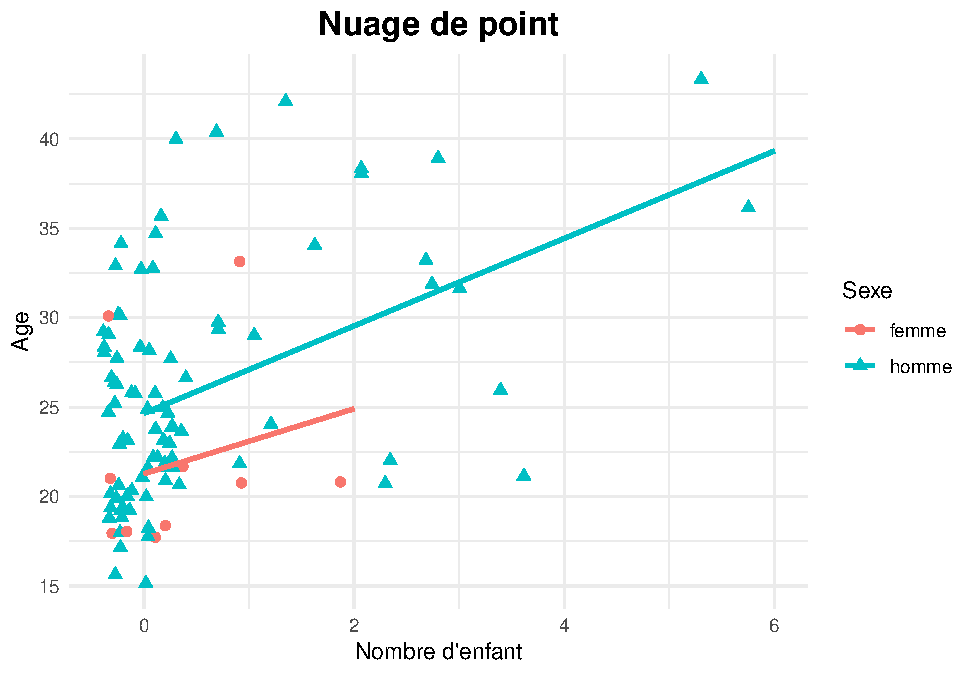
\includegraphics{PROJET_files/figure-latex/unnamed-chunk-35-1.pdf}

\newpage
\textcolor{blue}{\subsection{l’effet de l’appartenance au groupe de traitement sur l’intention de migrer}}

\begin{Shaded}
\begin{Highlighting}[]
\NormalTok{modele }\OtherTok{\textless{}{-}}\NormalTok{ stats}\SpecialCharTok{::}\FunctionTok{lm}\NormalTok{(endline\_intention }\SpecialCharTok{\textasciitilde{}}\NormalTok{ endline\_traitement, Fusion\_feuille)}


\NormalTok{modele }\SpecialCharTok{\%\textgreater{}\%} 
\NormalTok{  gtsummary}\SpecialCharTok{::}\FunctionTok{tbl\_regression}\NormalTok{(}
    \AttributeTok{label =} \FunctionTok{list}\NormalTok{(endline\_traitement }\SpecialCharTok{\textasciitilde{}} \StringTok{"TRAITEMENT"}\NormalTok{)}
\NormalTok{  )}\SpecialCharTok{\%\textgreater{}\%} 
  \FunctionTok{as\_flex\_table}\NormalTok{()}
\end{Highlighting}
\end{Shaded}

\global\setlength{\Oldarrayrulewidth}{\arrayrulewidth}

\global\setlength{\Oldtabcolsep}{\tabcolsep}

\setlength{\tabcolsep}{0pt}

\renewcommand*{\arraystretch}{1.5}



\providecommand{\ascline}[3]{\noalign{\global\arrayrulewidth #1}\arrayrulecolor[HTML]{#2}\cline{#3}}

\begin{longtable}[c]{|p{1.40in}|p{0.62in}|p{1.02in}|p{0.88in}}



\ascline{1pt}{000000}{1-4}

\multicolumn{1}{>{\raggedright}m{\dimexpr 1.4in+0\tabcolsep}}{\textcolor[HTML]{000000}{\fontsize{11}{11}\selectfont{\textbf{Caractéristique}}}} & \multicolumn{1}{>{\centering}m{\dimexpr 0.62in+0\tabcolsep}}{\textcolor[HTML]{000000}{\fontsize{11}{11}\selectfont{\textbf{Beta}}}} & \multicolumn{1}{>{\centering}m{\dimexpr 1.02in+0\tabcolsep}}{\textcolor[HTML]{000000}{\fontsize{11}{11}\selectfont{\textbf{95\%\ IC}}}\textcolor[HTML]{000000}{\textsuperscript{\fontsize{11}{11}\selectfont{1}}}} & \multicolumn{1}{>{\centering}m{\dimexpr 0.88in+0\tabcolsep}}{\textcolor[HTML]{000000}{\fontsize{11}{11}\selectfont{\textbf{p-valeur}}}} \\

\ascline{1pt}{000000}{1-4}\endhead



\multicolumn{4}{>{\raggedright}m{\dimexpr 3.91in+6\tabcolsep}}{\textcolor[HTML]{000000}{\textsuperscript{\fontsize{11}{11}\selectfont{1}}}\textcolor[HTML]{000000}{\fontsize{11}{11}\selectfont{IC\ =\ intervalle\ de\ confiance}}} \\

\endfoot



\multicolumn{1}{>{\raggedright}p{\dimexpr 1.4in+0\tabcolsep}}{\textcolor[HTML]{000000}{\fontsize{11}{11}\selectfont{TRAITEMENT}}} & \multicolumn{1}{>{\centering}p{\dimexpr 0.62in+0\tabcolsep}}{\textcolor[HTML]{000000}{\fontsize{11}{11}\selectfont{0,33}}} & \multicolumn{1}{>{\centering}p{\dimexpr 1.02in+0\tabcolsep}}{\textcolor[HTML]{000000}{\fontsize{11}{11}\selectfont{-0,37\ –\ 1,0}}} & \multicolumn{1}{>{\centering}p{\dimexpr 0.88in+0\tabcolsep}}{\textcolor[HTML]{000000}{\fontsize{11}{11}\selectfont{0,3}}} \\

\ascline{1pt}{000000}{1-4}



\end{longtable}



\arrayrulecolor[HTML]{000000}

\global\setlength{\arrayrulewidth}{\Oldarrayrulewidth}

\global\setlength{\tabcolsep}{\Oldtabcolsep}

\renewcommand*{\arraystretch}{1}

\textcolor{blue}{\subsection{Tableau de régression avec 3 modèles}}

\begin{Shaded}
\begin{Highlighting}[]
\NormalTok{Modele\_A }\OtherTok{=}\NormalTok{ modele }\SpecialCharTok{\%\textgreater{}\%} 
\NormalTok{  gtsummary}\SpecialCharTok{::}\FunctionTok{tbl\_regression}\NormalTok{()}

\NormalTok{Modele\_B }\OtherTok{=}\NormalTok{ stats}\SpecialCharTok{::}\FunctionTok{lm}\NormalTok{(}\AttributeTok{data =}\NormalTok{Fusion\_feuille,  endline\_traitement }\SpecialCharTok{\textasciitilde{}}\NormalTok{ endline\_age }\SpecialCharTok{+}\NormalTok{ endline\_sex) }\SpecialCharTok{\%\textgreater{}\%} 
\NormalTok{   gtsummary}\SpecialCharTok{::}\FunctionTok{tbl\_regression}\NormalTok{()}
  
\NormalTok{Modele\_C }\OtherTok{=}\NormalTok{ stats}\SpecialCharTok{::}\FunctionTok{lm}\NormalTok{(}\AttributeTok{data =}\NormalTok{Fusion\_feuille,  endline\_traitement }\SpecialCharTok{\textasciitilde{}}\NormalTok{ endline\_age }\SpecialCharTok{+}\NormalTok{ endline\_sex}\SpecialCharTok{+}\NormalTok{ endline\_district) }\SpecialCharTok{\%\textgreater{}\%} 
\NormalTok{  gtsummary}\SpecialCharTok{::}\FunctionTok{tbl\_regression}\NormalTok{()}

\NormalTok{gtsummary}\SpecialCharTok{::}\FunctionTok{tbl\_stack}\NormalTok{(}
  \FunctionTok{list}\NormalTok{(Modele\_A,}
\NormalTok{       Modele\_B,}
\NormalTok{       Modele\_C),}
  \AttributeTok{group\_header =} \FunctionTok{c}\NormalTok{(}\StringTok{"MODELE A"}\NormalTok{, }\StringTok{"MODELE B"}\NormalTok{, }\StringTok{"MODELE C"}\NormalTok{)}
\NormalTok{) }\SpecialCharTok{\%\textgreater{}\%} 
  \FunctionTok{as\_flex\_table}\NormalTok{()}
\end{Highlighting}
\end{Shaded}

\global\setlength{\Oldarrayrulewidth}{\arrayrulewidth}

\global\setlength{\Oldtabcolsep}{\tabcolsep}

\setlength{\tabcolsep}{0pt}

\renewcommand*{\arraystretch}{1.5}



\providecommand{\ascline}[3]{\noalign{\global\arrayrulewidth #1}\arrayrulecolor[HTML]{#2}\cline{#3}}

\begin{longtable}[c]{|p{1.08in}|p{1.54in}|p{0.63in}|p{1.10in}|p{0.88in}}



\ascline{1pt}{000000}{1-5}

\multicolumn{1}{>{\raggedright}m{\dimexpr 1.08in+0\tabcolsep}}{\textcolor[HTML]{000000}{\fontsize{11}{11}\selectfont{\textbf{Group}}}} & \multicolumn{1}{>{\raggedright}m{\dimexpr 1.54in+0\tabcolsep}}{\textcolor[HTML]{000000}{\fontsize{11}{11}\selectfont{\textbf{Caractéristique}}}} & \multicolumn{1}{>{\centering}m{\dimexpr 0.63in+0\tabcolsep}}{\textcolor[HTML]{000000}{\fontsize{11}{11}\selectfont{\textbf{Beta}}}} & \multicolumn{1}{>{\centering}m{\dimexpr 1.1in+0\tabcolsep}}{\textcolor[HTML]{000000}{\fontsize{11}{11}\selectfont{\textbf{95\%\ IC}}}\textcolor[HTML]{000000}{\textsuperscript{\fontsize{11}{11}\selectfont{1}}}} & \multicolumn{1}{>{\centering}m{\dimexpr 0.88in+0\tabcolsep}}{\textcolor[HTML]{000000}{\fontsize{11}{11}\selectfont{\textbf{p-valeur}}}} \\

\ascline{1pt}{000000}{1-5}\endhead



\multicolumn{5}{>{\raggedright}m{\dimexpr 5.24in+8\tabcolsep}}{\textcolor[HTML]{000000}{\textsuperscript{\fontsize{11}{11}\selectfont{1}}}\textcolor[HTML]{000000}{\fontsize{11}{11}\selectfont{IC\ =\ intervalle\ de\ confiance}}} \\

\endfoot



\multicolumn{1}{>{\raggedright}p{\dimexpr 1.08in+0\tabcolsep}}{\textcolor[HTML]{000000}{\fontsize{11}{11}\selectfont{MODELE\ A}}} & \multicolumn{1}{>{\raggedright}p{\dimexpr 1.54in+0\tabcolsep}}{\textcolor[HTML]{000000}{\fontsize{11}{11}\selectfont{endline\_traitement}}} & \multicolumn{1}{>{\centering}p{\dimexpr 0.63in+0\tabcolsep}}{\textcolor[HTML]{000000}{\fontsize{11}{11}\selectfont{0,33}}} & \multicolumn{1}{>{\centering}p{\dimexpr 1.1in+0\tabcolsep}}{\textcolor[HTML]{000000}{\fontsize{11}{11}\selectfont{-0,37\ –\ 1,0}}} & \multicolumn{1}{>{\centering}p{\dimexpr 0.88in+0\tabcolsep}}{\textcolor[HTML]{000000}{\fontsize{11}{11}\selectfont{0,3}}} \\





\multicolumn{1}{>{\raggedright}p{\dimexpr 1.08in+0\tabcolsep}}{\textcolor[HTML]{000000}{\fontsize{11}{11}\selectfont{MODELE\ B}}} & \multicolumn{1}{>{\raggedright}p{\dimexpr 1.54in+0\tabcolsep}}{\textcolor[HTML]{000000}{\fontsize{11}{11}\selectfont{endline\_age}}} & \multicolumn{1}{>{\centering}p{\dimexpr 0.63in+0\tabcolsep}}{\textcolor[HTML]{000000}{\fontsize{11}{11}\selectfont{0,00}}} & \multicolumn{1}{>{\centering}p{\dimexpr 1.1in+0\tabcolsep}}{\textcolor[HTML]{000000}{\fontsize{11}{11}\selectfont{0,00\ –\ 0,00}}} & \multicolumn{1}{>{\centering}p{\dimexpr 0.88in+0\tabcolsep}}{\textcolor[HTML]{000000}{\fontsize{11}{11}\selectfont{0,5}}} \\





\multicolumn{1}{>{\raggedright}p{\dimexpr 1.08in+0\tabcolsep}}{\textcolor[HTML]{000000}{\fontsize{11}{11}\selectfont{}}} & \multicolumn{1}{>{\raggedright}p{\dimexpr 1.54in+0\tabcolsep}}{\textcolor[HTML]{000000}{\fontsize{11}{11}\selectfont{endline\_sex}}} & \multicolumn{1}{>{\centering}p{\dimexpr 0.63in+0\tabcolsep}}{\textcolor[HTML]{000000}{\fontsize{11}{11}\selectfont{0,15}}} & \multicolumn{1}{>{\centering}p{\dimexpr 1.1in+0\tabcolsep}}{\textcolor[HTML]{000000}{\fontsize{11}{11}\selectfont{-0,18\ –\ 0,48}}} & \multicolumn{1}{>{\centering}p{\dimexpr 0.88in+0\tabcolsep}}{\textcolor[HTML]{000000}{\fontsize{11}{11}\selectfont{0,4}}} \\





\multicolumn{1}{>{\raggedright}p{\dimexpr 1.08in+0\tabcolsep}}{\textcolor[HTML]{000000}{\fontsize{11}{11}\selectfont{MODELE\ C}}} & \multicolumn{1}{>{\raggedright}p{\dimexpr 1.54in+0\tabcolsep}}{\textcolor[HTML]{000000}{\fontsize{11}{11}\selectfont{endline\_age}}} & \multicolumn{1}{>{\centering}p{\dimexpr 0.63in+0\tabcolsep}}{\textcolor[HTML]{000000}{\fontsize{11}{11}\selectfont{0,00}}} & \multicolumn{1}{>{\centering}p{\dimexpr 1.1in+0\tabcolsep}}{\textcolor[HTML]{000000}{\fontsize{11}{11}\selectfont{0,00\ –\ 0,00}}} & \multicolumn{1}{>{\centering}p{\dimexpr 0.88in+0\tabcolsep}}{\textcolor[HTML]{000000}{\fontsize{11}{11}\selectfont{0,5}}} \\





\multicolumn{1}{>{\raggedright}p{\dimexpr 1.08in+0\tabcolsep}}{\textcolor[HTML]{000000}{\fontsize{11}{11}\selectfont{}}} & \multicolumn{1}{>{\raggedright}p{\dimexpr 1.54in+0\tabcolsep}}{\textcolor[HTML]{000000}{\fontsize{11}{11}\selectfont{endline\_sex}}} & \multicolumn{1}{>{\centering}p{\dimexpr 0.63in+0\tabcolsep}}{\textcolor[HTML]{000000}{\fontsize{11}{11}\selectfont{0,14}}} & \multicolumn{1}{>{\centering}p{\dimexpr 1.1in+0\tabcolsep}}{\textcolor[HTML]{000000}{\fontsize{11}{11}\selectfont{-0,19\ –\ 0,47}}} & \multicolumn{1}{>{\centering}p{\dimexpr 0.88in+0\tabcolsep}}{\textcolor[HTML]{000000}{\fontsize{11}{11}\selectfont{0,4}}} \\





\multicolumn{1}{>{\raggedright}p{\dimexpr 1.08in+0\tabcolsep}}{\textcolor[HTML]{000000}{\fontsize{11}{11}\selectfont{}}} & \multicolumn{1}{>{\raggedright}p{\dimexpr 1.54in+0\tabcolsep}}{\textcolor[HTML]{000000}{\fontsize{11}{11}\selectfont{endline\_district}}} & \multicolumn{1}{>{\centering}p{\dimexpr 0.63in+0\tabcolsep}}{\textcolor[HTML]{000000}{\fontsize{11}{11}\selectfont{-0,02}}} & \multicolumn{1}{>{\centering}p{\dimexpr 1.1in+0\tabcolsep}}{\textcolor[HTML]{000000}{\fontsize{11}{11}\selectfont{-0,06\ –\ 0,02}}} & \multicolumn{1}{>{\centering}p{\dimexpr 0.88in+0\tabcolsep}}{\textcolor[HTML]{000000}{\fontsize{11}{11}\selectfont{0,4}}} \\

\ascline{1pt}{000000}{1-5}



\end{longtable}



\arrayrulecolor[HTML]{000000}

\global\setlength{\arrayrulewidth}{\Oldarrayrulewidth}

\global\setlength{\tabcolsep}{\Oldtabcolsep}

\renewcommand*{\arraystretch}{1}

\end{document}
